\documentclass[12pt,bibliography=oldstyle,DIV=12,parskip=half-]{scrreprt}


\iflatexml
% \documentclass[12pt,bibliography=oldstyle,DIV=12,parskip=half-]{scrreprt} % Not (yet) supported by LaTeXML.
\fi

\include{conf/preconfig}
\include{conf/packages}
\include{conf/config}
\include{conf/comandos}
\include{conf/fuentes}
% First macro on next line not (yet) supported by LaTeXML: 
% \addbibresource{res/bibliografia.bib}
\hyphenation{micro-RNA}
\hyphenation{micro-RNAs}
\hyphenation{mi-RNA}
\hyphenation{mi-RNAs}
% First macro on next line not (yet) supported by LaTeXML: 
% \addtokomafont{descriptionlabel}{\small}
% First macro on next line not (yet) supported by LaTeXML: 
% \setkomafont{subject}{\LARGE\usekomafont{disposition}}
% First macro on next line not (yet) supported by LaTeXML: 
% \setkomafont{title}{\normalfont\slshape}
% First macro on next line not (yet) supported by LaTeXML: 
% \setkomafont{subtitle}{\LARGE\usekomafont{disposition}}
\setlength{\abovecaptionskip}{-10pt plus 3pt minus 2pt}
\setlength{\belowcaptionskip}{10pt plus 3pt minus 2pt}
\hypersetup{
  colorlinks,
  citecolor=black,
  filecolor=black,
  linkcolor=black,
  urlcolor=black
}
% First macro on next line not (yet) supported by LaTeXML: 
% \sisetup{
%  table-number-alignment = right,
%  group-separator = ,
%  output-decimal-marker = {,},
%  retain-explicit-plus = true
%}
\newcommand{\e}[][]{\emph}

\newcommand{\fr}[1][]{(\autoref{#1})}

\newcommand{\iid}[][]{independiente e idénticamente distribuido}

\newtheorem{definicion}{Definición}[chapter]
\newtheorem{lema}[definicion]{Lema}
\newcommand{\ntA}[][]{\textrm{\mono{A}}{ }}

\newcommand{\ntC}[][]{\textrm{\mono{C}}{ }}

\newcommand{\ntG}[][]{\textrm{\mono{G}}{ }}

\newcommand{\ntU}[][]{\textrm{\mono{U}}{ }}

\newcommand{\pairL}[][]{\textrm{\mono{(}}{ }}

\newcommand{\pairR}[][]{\textrm{\mono{)}}{ }}

\newcommand{\noPair}[][]{\textrm{\mono{.}}{ }}

\newcommand{\dn}[1][]{\textrm{\mono{#1}}{ }}

\newcommand{\bp}[2][]{\textrm{\mono{#1-#2}}{ }}

\newcommand{\grad}[1][]{\nabla{#1}}

\newcommand{\tableStyle}[][]{\relsize{-0.5}\center\sffamily}

\newcommand{\captionStyle}[][]{\relsize{-0.5}}

\newcommand{\tE}[][]{&{\smaller $\bar{x}$}&}

\newcommand{\tF}[1][]{\multirow{2}{*}{#1}\tE}

\newcommand{\tZ}[][]{&{\smaller $\sigma$}&}

\newcommand{\tA}[][]{\addlinespace[4pt]}

\newcommand{\rowMEAN}[1][]{&\multirow{2}{*}{#1}&{\smaller $\bar{x}$}}

\newcommand{\rowSTD}[][]{&&{\smaller $\sigma$}}

\newcommand{\rowSKIP}[][]{\addlinespace[2pt]}

\newcommand{\ti}[][]{\textsmaller}

\newcommand{\func}[1][]{\emph{#1}}

\newcommand{\Gm}[][]{\scriptsize $G_m$}

\newcommand{\Ft}[1][]{\mrow{2}{*}{#1}}

\newcommand{\tbmean}[][]{\smaller{2} $\bar{x}$}

\newcommand{\tbstd}[][]{\smaller $\sigma$}

\newcommand{\tripletsvm}[][]{\sbsf{Triplet-SVM}}

\newcommand{\mipred}[][]{\sbsf{miPred}}

\newcommand{\micropred}[][]{\sbsf{microPred}}

\newcommand{\deltamirbase}[][]{\sbsf{$\mathbf{\mathsf{\Delta}}$miRBase}}

\newcommand{\rowMEANN}[2][]{&
  \multirow{2}{*}{\tablenum[table-format=1.0,table-number-alignment=right]{#1}}&
  \multirow{2}{*}{\tablenum[table-format=3.0,table-number-alignment=right]{#2}}&
           {\smaller $\bar{x}$}}

\newcommand{\rowSTDN}[][]{&&&{\smaller $\sigma$}}

% First macro on next line not (yet) supported by LaTeXML: 
% \DeclareSIUnit\nt{nt}
\newcommand{\VP}[][]{\T{\textsl{VP}}}
\newcommand{\VN}[][]{\T{\textsl{VN}}}
\newcommand{\FP}[][]{\T{\textsl{FP}}}
\newcommand{\FN}[][]{\T{\textsl{FN}}}
\newcommand{\SE}[][]{\T{\textsl{SE}}}
\newcommand{\SP}[][]{\T{\textsl{SP}}}
\newcommand{\GM}[][]{\T{\textsl{Gm}}}
\newcommand{\PR}[][]{\T{\textsl{Pr}}}
\newcommand{\AC}[][]{\T{\textsl{Ac}}}
\newcommand{\feedforward}[][]{con propagación hacia adelante}
\newcommand{\headRow}[][]{  \sfbf{\footnotesize Pos.} &
  \sfbf{\footnotesize Característica} &
  \sfbf{\footnotesize Descripción}
}
\newcommand{\tripletRow}[1][]{
  \stepcounter{FeatureCounter}\theFeatureCounter & $N_{\T{\mono{#1}}}$
  & Ocurrencias del triplete \mono{#1} en la región del tallo.}
\newcommand{\dnRow}[1][]{
  \stepcounter{FeatureCounter}\theFeatureCounter & $N_{\T{\mono{#1}}}$
  & Número de dinucleótidos \mono{#1} en la secuencia.}
\newcommand{\funcheader}[3][]{\begin{description}%
  \item[Función]{#1}\item[Entradas]{#2}\item[Salidas]{#3}%
\end{description}}
\renewcommand{\bibfont}[][]{\normalfont\footnotesize}

\iflatexml\else\ohead{\small capitulo3-tmp, rev. 2e32658+, \today}\fi

\begin{document}
\selectlanguage{spanish}
\title{Informe Final - Capítulo 3}

%
\begin{abstract}
%
DevOps es un conjunto de prácticas y principios utilizados para
agilizar la producción del software. Busca generar una cultura en
común dentro de las organizaciones integrando el trabajo de las
diferentes áreas involucradas en la producción y entrega del
software. Propone aprovechar la automatización para eliminar trabajo
innecesario de las personas, y destaca la importancia de establecer un
proceso de mejora continua basado en objetivos medibles y
verificables.
  
En este Proyecto se implementaron prácticas y herramientas
tecnológicas en busca de integrar el trabajo de desarrollo y
operaciones de acuerdo a la propuesta DevOps. El trabajo incluyó la
automatización de tareas de infraestructura, la implementación de
tuberías de integración y entrega continuas y la unificación de los
repositorios de código fuente y configuración. Asimismo, se
implementaron herramientas para brindar autoservicio de la
infraestructura, visibilidad de métricas y registros y
comunicación. El ámbito de trabajo fue la Dirección de Informatización
y Planificación Tecnológica de la Universidad Nacional del Litoral
(DIPT-UNL).
%
\end{abstract}
%

\titlehead{\center\large
\includegraphics[width=4cm]{figures/logofichunl/logofichunl.pdf}\smallskip\\
 Universidad Nacional del Litoral\\
 Facultad de Ingeniería y Ciencias Hídricas
}

\subject{
 Proyecto Final de Carrera\\
 Ingeniería en Informática
}
\subtitle{
}

\publishers{
}

\date{\today}

\author{  Alumno: Mauro J. Torrez\\
  Directora: Ing. Claudia S. Arrietti
}

\dedication{\normalfont\normalsize\itshape
A mis padres, gracias a su esfuerzo y apoyo hoy estoy aquí.

A mis hermanos y a mis amigos, quienes me acompañaron durante todo
este tiempo.

A mi directora, por la confianza en este proyecto.

A mi madrina, por alentarme siempre a trabajar para alcanzar este
objetivo.

A mi abuela Nydia, quien hubiera sido la persona más orgullosa de este
logro.
}

\renewcommand*{\titlepagestyle}{empty}
\maketitle

%
%
%
\chapter{Introducción}
\setcounter{page}{1}
%
En este Informe se describe el desarrollo de un método para la
clasificación de secuencias de \premirna{}, un tipo específico de
ácido ribonucleico (\e{RNA}, del inglés \eng{ribonucleic acid}),
mediante la utilización de Perceptrones Multicapa (MLPs) y Máquinas de
Vectores de Soporte (SVMs), técnicas de la Inteligencia Computacional
para el aprendizaje automático.

La Inteligencia Computacional es la disciplina que estudia la
aplicación de técnicas inspiradas en la naturaleza para resolver
problemas computacionales.
Dentro de su área de interés, la clasificación automática
es una de las aplicaciones más difundidas.
Las técnicas MLP y SVM utilizadas en el presente Trabajo implementan
el aprendizaje supervisado, generando ``modelos'' capaces de
discriminar entre diferentes tipos de datos, a partir de ejemplos que
se ``enseñan'' a la máquina.
La utilización de medios automáticos de clasificación resulta de
interés para tareas que involucran grandes volúmenes de datos, sobre
los cuales resulta imposible un tratamiento manual.
La identificación de secuencias de \premirna{s} --y de
cadenas de ácidos nucleicos en general-- es una tarea que
presenta estas \caract{s}.
%% Los ácidos ribonucleicos (ARN o RNA, del inglés \e{ribonucleic acid})
%% son un tipo de ácido nucleico formado por una cadena de nucleótidos,
%% cada uno de los cuales contiene una de las cuatro bases nitrogenadas:
%% adenina, guanina, citosina y uracilo.
%%
%% La naturaleza secuencial de los RNA hace que su representación
%% computacional sea sencilla, en forma de cadenas de caracteres que
%% representan la base de cada nucleótido.

%
%
%
\section{Acerca de los (pre-)miRNAs}
%
Los miRNAs, también conocidos como microRNAs, son pequeñas moléculas
de ácido ribonucleico (\eng{RNA}, del inglés \e{ribonucleic acid})
compuestas por una cadena de unos $22$ nucleótidos $[\nt{}]$ de
longitud.
Hace aproximadamente una década se propuso que estas moléculas, hasta
el momento ignoradas aunque presentes en grandes cantidades en la
célula, jugarían un papel decisivo en la reproducción celular,
promoviendo la diferenciación en distintos tipos de tejidos y/o su
permanencia en un estado particular de diferenciación
\cite{lee-mammal}.
Estudios posteriores han demostrado que los miRNAs ejercen una función
reguladora de la expresión génica celular \cite{bartel116} y están
involucrados en varios procesos genéticos dentro de la célula, como la
transcripción de mRNAs (\e{RNA mensajeros}) y la síntesis de proteínas
\cite{lili}.
Este efecto regulador puede tener gran implicancia en el desarrollo y
evolución de la enfermedad celular.
Se ha demostrado que los miRNAs juegan un rol importante en la
carcinogénesis \cite{aurora,lili}, regulando la proliferación y muerte
celular, entre otras funciones tales como el metabolismo de las grasas
en moscas, los procesos de infección viral, y el control del
desarrollo de flores y hojas en plantas \cite{bartel116,lecellier}.

El debate acerca del número e identidad de los miRNAs presentes en
diferentes genomas es una cuestión abierta: a modo de ejemplo, para el
caso del genoma humano se había estimado inicialmente que se
encontrarían unos pocos cientos de genes miRNA; posteriormente este
número ha sido revisado a unos 1000 \cite{sewer,chang}.
Actualmente, se encuentra que el número de miRNAs descubiertos en
humanos duplica esta cifra \cite{gomes}.
Asimismo, este número podría ser mucho mayor si se considera que
existen miRNAs de evolución más reciente, específicos a la especie
humana \cite{sewer}.

Los miRNAs se presentan naturalmente dentro de una molécula denominada
pre-miRNA o \e{miRNA precursor}, de unos $70\,\nt$ de longitud, la
cual contiene uno o más miRNAs (llamados \e{maduros}) en su secuencia.
En la \iflatexml{}Figura~\ref{horquilla}\else\autoref{horquilla}\fi{}
se representa en forma esquemática la secuencia de una cadena de
pre-miRNA y su correspondiente \e{estructura secundaria}.
Esta estructura secundaria viene dada por la forma en que la cadena de
nucleótidos se \e{pliega} sobre sí misma logrando estabilidad
molecular.
Tal como en el ejemplo de la
\iflatexml{}Figura~\ref{horquilla}\else\autoref{horquilla}\fi, en el
reino animal la estructura secundaria típica de un pre-miRNA conforma
una especie de \e{horquilla} \cite{bartel116,sewer}.

\begin{figure}[t]
\figureStyle
%\includegraphics[width=\textwidth]{figures/hsa-mir-299_ss/hsa-mir-299_ss.pdf}
%nnodes = 75
\shorthandoff{<}
\shorthandoff{>}
\tikzsetnextfilename{figures/hsa-mir-299_ss/hsa-mir-299_ss}
\begin{tikzpicture}[scale=0.025,rotate=90,font=\relscale{0.9}\sffamily,
    every label/.style={label distance=0}]
\definecolor{rosa}{rgb}{0.78,0,0.45};
\definecolor{verde}{rgb}{0,0.63,0.51};
\definecolor{ro}{rgb}{0.78,0,0.45};
\definecolor{ve}{rgb}{0,0.63,0.51};
%\definecolor{}{rgb}{0,0,0};

\tikzstyle{lstyle}=[shorten >= 2,shorten <= 2];
  \foreach \q / \colr [count=\c] in {
 A/black, A/black, G/black, A/black, A/black, A/black, U/ro, G/ro,
 G/ro, U/ro, U/ro, U/ro, A/ro, C/ro, C/ro, G/ro, U/ro, C/ro, C/ro,
 C/ro, A/ro, C/ro, A/ro, U/ro, A/ro, C/ro, A/ro, U/ro, U/black,
 U/black, U/black, G/black, A/black, A/black, U/black, A/black,
 U/black, G/black, U/ve, A/ve, U/ve, G/ve, U/ve, G/ve, G/ve, G/ve,
 A/ve, U/ve, G/ve, G/ve, U/ve, A/ve, A/ve, A/ve, C/ve, C/ve, G/ve,
 C/ve, U/ve, U/ve, C/black, U/black, U/black} {
    \pgfmathsetmacro\cpos{ 240 - \c * 9 };
    \node[anchor=center,color={\colr}] (ns\c)
    at (180,\cpos) {\q};
  }

  %%%%%%%%%%%%%%%%%%%%%%%%%%%%%%%%%%%%%%%%%%%%%%%%%%%%%%%%%%%%%%%%%%%%


\coordinate[label={[xshift=0,yshift=0]below:A}] (1) at (92.5000,172.2035);
\fill[] (1) circle (2.2);
\coordinate[label={[xshift=0,yshift=0]below:A}] (2) at (92.5000,157.2035);
\fill[] (2) circle (1.1);
\coordinate[label={[xshift=0,yshift=0]below:G}] (3) at (92.5000,142.2035);
\fill[] (3) circle (1.1);
\coordinate[label={[xshift=0,yshift=0]below:A}] (4) at (92.5000,127.2035);
\fill[] (4) circle (1.1);
\coordinate[label={[xshift=0,yshift=0]below:A}] (5) at (92.5000,112.2035);
\fill[] (5) circle (1.1);
\coordinate[label={[xshift=0,yshift=0]below:A}] (6) at (85.6761,100.0000);
\fill[] (6) circle (1.1);
\coordinate[label={[xshift=0,yshift=0,rosa]below:U}] (7) at (92.5000,87.7965);
\fill[] (7) circle (1.1);
\coordinate[label={[xshift=0,yshift=0,rosa]below:G}] (8) at (92.5000,72.7965);
\fill[] (8) circle (1.1);
\coordinate[label={[xshift=0,yshift=0,rosa]below:G}] (9) at (92.5000,57.7965);
\fill[] (9) circle (1.1);
\coordinate[label={[xshift=0,yshift=0,rosa]below:U}] (10) at (92.5000,42.7965);
\fill[] (10) circle (1.1);
\coordinate[label={[xshift=0,yshift=0,rosa]below:U}] (11) at (92.5000,27.7965);
\fill[] (11) circle (1.1);
\coordinate[label={[xshift=0,yshift=0,rosa]below:U}] (12) at (92.5000,12.7965);
\fill[] (12) circle (1.1);
\coordinate[label={[xshift=0,yshift=0,rosa]below:A}] (13) at (92.5000,-2.2035);
\fill[] (13) circle (1.1);
\coordinate[label={[xshift=0,yshift=0,rosa]below:C}] (14) at (92.5000,-17.2035);
\fill[] (14) circle (1.1);
\coordinate[label={[xshift=0,yshift=0,rosa]below:C}] (15) at (92.5000,-32.2035);
\fill[] (15) circle (1.1);
\coordinate[label={[xshift=0,yshift=0,rosa]below:G}] (16) at (92.5000,-47.2035);
\fill[] (16) circle (1.1);
\coordinate[label={[xshift=0,yshift=0,rosa]below:U}] (17) at (92.5000,-62.2035);
\fill[] (17) circle (1.1);
\coordinate[label={[xshift=0,yshift=0,rosa]below:C}] (18) at (92.5000,-77.2035);
\fill[] (18) circle (1.1);
\coordinate[label={[xshift=0,yshift=0,rosa]below:C}] (19) at (92.5000,-92.2035);
\fill[] (19) circle (1.1);
\coordinate[label={[xshift=0,yshift=0,rosa]below:C}] (20) at (92.5000,-107.2035);
\fill[] (20) circle (1.1);
\coordinate[label={[xshift=0,yshift=0,rosa]below:A}] (21) at (92.5000,-122.2035);
\fill[] (21) circle (1.1);
\coordinate[label={[xshift=0,yshift=0,rosa]below:C}] (22) at (92.5000,-137.2035);
\fill[] (22) circle (1.1);
\coordinate[label={[xshift=0,yshift=0,rosa]below:A}] (23) at (92.5000,-152.2035);
\fill[] (23) circle (1.1);
\coordinate[label={[xshift=0,yshift=0,rosa]below:U}] (24) at (92.5000,-167.2035);
\fill[] (24) circle (1.1);
\coordinate[label={[xshift=0,yshift=0,rosa]below:A}] (25) at (92.5000,-182.2035);
\fill[] (25) circle (1.1);
\coordinate[label={[xshift=0,yshift=0,rosa]below:C}] (26) at (92.5000,-197.2035);
\fill[] (26) circle (1.1);
\coordinate[label={[xshift=0,yshift=0,rosa]below:A}] (27) at (92.5000,-212.2035);
\fill[] (27) circle (1.1);
\coordinate[label={[xshift=-2,yshift=0,rosa]below:U}] (28) at (92.5000,-227.2035);
\fill[] (28) circle (1.1);
\coordinate[label={[xshift=-2,yshift=0]below:U}] (29) at (80.4054,-237.1159);
\fill[] (29) circle (1.1);
\coordinate[label={[xshift=2,yshift=0]below:U}] (30) at (77.5628,-252.4929);
\fill[] (30) circle (1.1);
\coordinate[label={[xshift=6,yshift=4]below:U}] (31) at (85.3143,-266.0741);
\fill[] (31) circle (1.1);
\coordinate[label={[xshift=0,yshift=0]right:G}] (32) at (100.0000,-271.4467);
\fill[] (32) circle (1.1);
\coordinate[label={[xshift=6,yshift=-4]above:A}] (33) at (114.6857,-266.0741);
\fill[] (33) circle (1.1);
\coordinate[label={[xshift=2,yshift=0]above:A}] (34) at (122.4372,-252.4929);
\fill[] (34) circle (1.1);
\coordinate[label={[xshift=-2,yshift=0]above:U}] (35) at (119.5946,-237.1159);
\fill[] (35) circle (1.1);
\coordinate[label={[xshift=-2,yshift=0]above:A}] (36) at (107.5000,-227.2035);
\fill[] (36) circle (1.1);
\coordinate[label={[xshift=0,yshift=0]above:U}] (37) at (107.5000,-212.2035);
\fill[] (37) circle (1.1);
\coordinate[label={[xshift=0,yshift=0]above:G}] (38) at (107.5000,-197.2035);
\fill[] (38) circle (1.1);
\coordinate[label={[xshift=0,yshift=0,verde]above:U}] (39) at (107.5000,-182.2035);
\fill[] (39) circle (1.1);
\coordinate[label={[xshift=0,yshift=0,verde]above:A}] (40) at (107.5000,-167.2035);
\fill[] (40) circle (1.1);
\coordinate[label={[xshift=0,yshift=0,verde]above:U}] (41) at (107.5000,-152.2035);
\fill[] (41) circle (1.1);
\coordinate[label={[xshift=0,yshift=0,verde]above:G}] (42) at (107.5000,-137.2035);
\fill[] (42) circle (1.1);
\coordinate[label={[xshift=0,yshift=0,verde]above:U}] (43) at (107.5000,-122.2035);
\fill[] (43) circle (1.1);
\coordinate[label={[xshift=0,yshift=0,verde]above:G}] (44) at (107.5000,-107.2035);
\fill[] (44) circle (1.1);
\coordinate[label={[xshift=0,yshift=0,verde]above:G}] (45) at (107.5000,-92.2035);
\fill[] (45) circle (1.1);
\coordinate[label={[xshift=0,yshift=0,verde]above:G}] (46) at (107.5000,-77.2035);
\fill[] (46) circle (1.1);
\coordinate[label={[xshift=0,yshift=0,verde]above:A}] (47) at (107.5000,-62.2035);
\fill[] (47) circle (1.1);
\coordinate[label={[xshift=0,yshift=0,verde]above:U}] (48) at (107.5000,-47.2035);
\fill[] (48) circle (1.1);
\coordinate[label={[xshift=0,yshift=0,verde]above:G}] (49) at (107.5000,-32.2035);
\fill[] (49) circle (1.1);
\coordinate[label={[xshift=0,yshift=0,verde]above:G}] (50) at (107.5000,-17.2035);
\fill[] (50) circle (1.1);
\coordinate[label={[xshift=0,yshift=0,verde]above:U}] (51) at (107.5000,-2.2035);
\fill[] (51) circle (1.1);
\coordinate[label={[xshift=0,yshift=0,verde]above:A}] (52) at (107.5000,12.7965);
\fill[] (52) circle (1.1);
\coordinate[label={[xshift=0,yshift=0,verde]above:A}] (53) at (107.5000,27.7965);
\fill[] (53) circle (1.1);
\coordinate[label={[xshift=0,yshift=0,verde]above:A}] (54) at (107.5000,42.7965);
\fill[] (54) circle (1.1);
\coordinate[label={[xshift=0,yshift=0,verde]above:C}] (55) at (107.5000,57.7965);
\fill[] (55) circle (1.1);
\coordinate[label={[xshift=0,yshift=0,verde]above:C}] (56) at (107.5000,72.7965);
\fill[] (56) circle (1.1);
\coordinate[label={[xshift=0,yshift=0,verde]above:G}] (57) at (107.5000,87.7965);
\fill[] (57) circle (1.1);
\coordinate[label={[xshift=0,yshift=0,verde]above:C}] (58) at (114.3239,100.0000);
\fill[] (58) circle (1.1);
\coordinate[label={[xshift=0,yshift=0,verde]above:U}] (59) at (107.5000,112.2035);
\fill[] (59) circle (1.1);
\coordinate[label={[xshift=0,yshift=0,verde]above:U}] (60) at (107.5000,127.2035);
\fill[] (60) circle (1.1);
\coordinate[label={[xshift=0,yshift=0]above:C}] (61) at (107.5000,142.2035);
\fill[] (61) circle (1.1);
\coordinate[label={[xshift=0,yshift=0]above:U}] (62) at (107.5000,157.2035);
\fill[] (62) circle (1.1);
\coordinate[label={[xshift=0,yshift=0]above:U}] (63) at (107.5000,172.2035);
\fill[] (63) circle (1.1);
\draw[lstyle] (1) -- (2);
\draw[lstyle] (2) -- (3);
\draw[lstyle] (3) -- (4);
\draw[lstyle] (4) -- (5);
\draw[lstyle] (5) -- (6);
\draw[lstyle] (6) -- (7);
\draw[lstyle] (7) -- (8);
\draw[lstyle] (8) -- (9);
\draw[lstyle] (9) -- (10);
\draw[lstyle] (10) -- (11);
\draw[lstyle] (11) -- (12);
\draw[lstyle] (12) -- (13);
\draw[lstyle] (13) -- (14);
\draw[lstyle] (14) -- (15);
\draw[lstyle] (15) -- (16);
\draw[lstyle] (16) -- (17);
\draw[lstyle] (17) -- (18);
\draw[lstyle] (18) -- (19);
\draw[lstyle] (19) -- (20);
\draw[lstyle] (20) -- (21);
\draw[lstyle] (21) -- (22);
\draw[lstyle] (22) -- (23);
\draw[lstyle] (23) -- (24);
\draw[lstyle] (24) -- (25);
\draw[lstyle] (25) -- (26);
\draw[lstyle] (26) -- (27);
\draw[lstyle] (27) -- (28);
\draw[lstyle] (28) -- (29);
\draw[lstyle] (29) -- (30);
\draw[lstyle] (30) -- (31);
\draw[lstyle] (31) -- (32);
\draw[lstyle] (32) -- (33);
\draw[lstyle] (33) -- (34);
\draw[lstyle] (34) -- (35);
\draw[lstyle] (35) -- (36);
\draw[lstyle] (36) -- (37);
\draw[lstyle] (37) -- (38);
\draw[lstyle] (38) -- (39);
\draw[lstyle] (39) -- (40);
\draw[lstyle] (40) -- (41);
\draw[lstyle] (41) -- (42);
\draw[lstyle] (42) -- (43);
\draw[lstyle] (43) -- (44);
\draw[lstyle] (44) -- (45);
\draw[lstyle] (45) -- (46);
\draw[lstyle] (46) -- (47);
\draw[lstyle] (47) -- (48);
\draw[lstyle] (48) -- (49);
\draw[lstyle] (49) -- (50);
\draw[lstyle] (50) -- (51);
\draw[lstyle] (51) -- (52);
\draw[lstyle] (52) -- (53);
\draw[lstyle] (53) -- (54);
\draw[lstyle] (54) -- (55);
\draw[lstyle] (55) -- (56);
\draw[lstyle] (56) -- (57);
\draw[lstyle] (57) -- (58);
\draw[lstyle] (58) -- (59);
\draw[lstyle] (59) -- (60);
\draw[lstyle] (60) -- (61);
\draw[lstyle] (61) -- (62);
\draw[lstyle] (62) -- (63);
\draw[lstyle] (1) -- (63);
\draw[lstyle] (2) -- (62);
\draw[lstyle] (3) -- (61);
\draw[lstyle] (4) -- (60);
\draw[lstyle] (5) -- (59);
\draw[lstyle] (7) -- (57);
\draw[lstyle] (8) -- (56);
\draw[lstyle] (9) -- (55);
\draw[lstyle] (10) -- (54);
\draw[lstyle] (11) -- (53);
\draw[lstyle] (12) -- (52);
\draw[lstyle] (13) -- (51);
\draw[lstyle] (14) -- (50);
\draw[lstyle] (15) -- (49);
\draw[lstyle] (16) -- (48);
\draw[lstyle] (17) -- (47);
\draw[lstyle] (18) -- (46);
\draw[lstyle] (19) -- (45);
\draw[lstyle] (20) -- (44);
\draw[lstyle] (21) -- (43);
\draw[lstyle] (22) -- (42);
\draw[lstyle] (23) -- (41);
\draw[lstyle] (24) -- (40);
\draw[lstyle] (25) -- (39);
\draw[lstyle] (26) -- (38);
\draw[lstyle] (27) -- (37);
\draw[lstyle] (28) -- (36);
\end{tikzpicture}
\shorthandon{<}
\shorthandon{>}


\caption{\captionStyle\protect\label{horquilla}
Secuencia (arriba) y estructura secundaria tipo horquilla (abajo) del
pre-miRNA de la especie humana \textbf{hsa-mir-299}.
}
\end{figure}
La forma clásica de identificación de nuevos \premirna{s} son las
pruebas experimentales de laboratorio.
Sin embargo, este tipo de pruebas sólo pueden identificar con
fiabilidad aquellos \premirna{s} abundantes dentro de la célula.
Las técnicas computacionales son una alternativa a las pruebas de
laboratorio que superan estas dificultades, ya que al extraer la
información directamente a partir del genoma de cada organismo,
permiten encontrar aquellos \premirna{s} que son específicos a
determinados tipos de tejidos o estadíos de desarrollo celular, y
aquellos escasamente expresados \cite{ding,sheng,xu}.

%
%
%
\section{Clasificación de \premirna{s}}
%
En el ámbito de la Inteligencia Computacional se han desarrollado
diversas técnicas de \e{aprendizaje supervisado} que pueden ser
utilizadas para la clasificación de \premirna{s}.
A grandes rasgos, estas técnicas generan una representación interna
(\e{modelo}) que caracteriza los \premirna{s}, extrayendo información
a partir de un conjunto de datos de ejemplo denominado \e{conjunto de
  entrenamiento}.
Una vez ``entrenado'', el modelo puede ser aplicado sobre nuevos
ejemplos para obtener predicciones de \e{clase}, asociando una clase
``positiva'' a los ejemplos de \premirna{s}, y una clase ``negativa''
a los ejemplos que son de otro tipo.
Esta propiedad se denomina \e{capacidad de generalización}.

En el presente trabajo se utilizan las técnicas de aprendizaje
supervisado llamadas \e\MVS{} \cite{svm} y \e{perceptrón multicapa}
\cite{mlp1,mlp2} como clasificadores de secuencias de \premirna{s}.
Mientras que la primera es la técnica más ampliamente utilizada en
la disciplina para la clasificación, el uso del perceptrón multicapa
resulta novedoso en este tipo de problemas, y se hipotetiza que podría
alcanzar un mejor desempeño que la máquina de vectores de soporte.

El perceptrón multicapa (\e{MLP}, del inglés \eng{Multi-Layer
  Perceptron}) es un tipo de red neuronal artificial con propagación
hacia adelante en la que se disponen nodos computadores (llamados
\e{neuronas}) organizados en \e{capas}.
La salida de cada neurona se determina a partir de una suma ponderada
de las salidas en la capa anterior.
Durante el entrenamiento del perceptrón multicapa, se ajustan
progresivamente los pesos (ponderaciones) de cada neurona mediante un
algoritmo de aprendizaje basado en la \e{propagación hacia atrás} del
error de clasificación, hasta satisfacer un criterio de corte
\cite{jain}.

La \MVS{} (\e{SVM}, de su nombre en inglés \eng{Support Vector
  Machine}) es un algoritmo de clasificación que, considerando a los
ejemplos como puntos en un espacio vectorial, determina un hiperplano
óptimo de separación que permite discriminar la clase de los ejemplos
según se encuentren a un lado u otro del hiperplano.
Aplicando unas funciones denominadas \e{núcleos}, esta operación se
efectúa de manera implícita en un espacio vectorial transformado de
alta dimensionalidad, en el que se espera que los ejemplos sean
linealmente separables \cite{bottou}.

%
%
%
\section{Motivación}
%
Este proyecto se origina en el Centro de Investigación en Señales, 
Sistemas e Inteligencia Computacional \e{sinc(i)} ante la necesidad de
contar con  una herramienta de clasificación de \premirna{s}, que sea
de fácil utilización por parte del usuario no experto en Inteligencia
Computacional.

%Con este desarrollo se pretende que los especialistas \hl{especificar}
%cuenten con una herramienta sencilla para la aplicación de técnicas
%avanzadas de clasificación, e integrada a su flujo de trabajo
%habitual.

%
%
%
\section{Objetivos}
%
El objetivo general del proyecto es desarrollar un método de
clasificación de \premirna{s} aplicando las técnicas de
perceptrón multicapa (MLP) y máquinas de vectores de soporte(SVM).
El software desarrollado debe abarcar todo el proceso desde
la lectura de los datos de entrada en un formato estándar hasta la
obtención de predicciones de clase para nuevos ejemplos.

%Adicionalmente, se pretende que el método desarrollado tenga un alto
%grado de automatización de los aspectos que no sean especialidad del
%usuario final, brindando facilidad de uso con buenos resultados de
%clasificación.

%
%
\subsection{Objetivos específicos}
%
\begin{itemize}
\item Recopilar bases de datos con ejemplos de clase positiva y
  negativa.
\item Diseñar y codificar un método de extracción de \caract{s} sobre
  estos datos replicando técnicas presentes en la bibliografía.
\item Diseñar y codificar métodos para la generación del modelo del
  clasificador, determinando parámetros adecuados para el
  entrenamiento. 
\item Diseñar y codificar los métodos necesarios para la clasificación
  aplicando el modelo generado sobre nuevos datos.
\item Codificar y documentar una interfaz de línea de comandos, y una
  interfaz web orientada al usuario final.
\item Efectuar pruebas del método final con los datos disponibles y
  documentar los resultados obtenidos.
\end{itemize}
%

%
%
%
\section{Alcances}
%
\begin{itemize}
\item
  El desarrollo se centra en la etapa de generación del modelo
  y su aplicación como clasificador, haciendo uso de la técnicas de
  máquina de vectores de soporte (SVM) y perceptrón multicapa
  (MLP).
\item
  Se trabajará durante el desarrollo exclusivamente con datos que se
  encuentren disponibles en línea, y cuya pertenencia de clase sea
  conocida.
\item
  No se pretende innovar en el campo de la extracción de \caract{s},
  por lo que en el desarrollo se replicarán técnicas propuestas
  por otros autores.
\item
  El objetivo del software a desarrollar es la identificación de
  \premirna{s}, quedando fuera del alcance de este proyecto la
  identificación de los miRNAs maduros contenidos dentro de los 
  mismos.
\item
  El proyecto no persigue el desarrollo de un producto o servicio
  comercial.
\end{itemize}
%

\chapter{Fundamentos teóricos}

DevOps es un movimiento cultural que busca mejorar el software como
producto así como también la vida de quienes se dedican a su
producción. Su propuesta es aplicar las prácticas y principios más
fiables del mundo de la manufactura de productos físicos a las
Tecnologías de la Información (TI)
\cite{handbook}. Sus
fundamentos provienen de áreas tales como \e{lean}\footnote{ El
  adjetivo inglés \e{lean} (/li:n/) puede traducirse como ligero,
  esbelto, despojado.} \cite{lean}, la teoría de
las limitaciones
\cite{thegoal}, el sistema de
producción de Toyota
\cite{toyota}, y el
aprendizaje organizacional
\cite{fifth}. El resultado
es la producción de software de alta calidad, confiable, estable y
seguro, en un ambiente de trabajo saludable y con un bajo costo
económico.

Entre los beneficios comúnmente atribuidos a una adopción de prácticas
DevOps podemos citar
\cite{awsdevops}:

\begin{itemize}
\item \e{Velocidad}: los equipos de desarrollo gestionan sus
  servicios mediante la automatización de la infraestructura y la
  integración continua.
\item \e{Entrega rápida}: la reducción del tamaño de las
  actualizaciones junto con la integración continua y la entrega
  continua aumentan la velocidad de llegada de los requerimientos a
  los clientes.
\item \e{Confiabilidad}: la integración continua efectúa pruebas
  del software constantemente haciendo que los problemas se detecten
  antes. Las herramientas de monitoreo proveen retroalimentación
  (\e{feedback}) sobre el funcionamiento del software.
\item \e{Colaboración}: la cultura DevOps enfatiza valores como
  la propiedad y la responsabilidad. Los equipos de desarrollo y de
  operaciones colaboran estrechamente, comparten muchas
  responsabilidades y combinan sus flujos de trabajo.
\end{itemize}
\section{Contexto histórico}

Si bien el origen de DevOps se identifica en el movimiento
\e{lean}, muchos lo reconocen como la continuación lógica de la
propuesta del desarrollo ágil que revolucionó la ingeniería de
software allá por 2001
\cite{agilemanifesto}.

A continuación se presenta un breve repaso de los contextos, los
eventos, y las personas de los que surgieron las ideas que dan forma a
la propuesta DevOps.

\subsection{Los comienzos}

En los comienzos, la persona encargada del desarrollo de software se
encargaba también de su operación. Jean Bartik, programadora de la
primera computadora de uso general ENIAC, aprendió a programarla a
partir de sus diagramas de circuitos. Programar la computadora
requería ajustar perillas y cambiar conexiones de cables, algo que hoy
en día asociamos más a la idea de operación.

Con el avance de las capacidades del hardware, éste pasó a dejar de
ser un impedimento, lo cual posibilitó el desarrollo de software de
mayor complejidad. Desde la década de los 60 hasta finales de los 80
tuvo lugar la llamada \e{crisis del software}, en la que se
identificaron los problemas del desarrollo. Esto dio origen a la
disciplina de ingeniería de software, que estableció un marco teórico
y propuso métodos para la producción del software.

En los años 90, el auge de internet puso en evidencia los problemas de
los métodos tradicionales de ingeniería de software: se necesitaba
responder a las demandas de los usuarios con mayor rapidez. La
operación del software en línea pasó de ser una tarea secundaria a un
aspecto crítico.

\subsection{El movimiento \e{lean}}

En los años 80, el sistema de producción de Toyota inventó técnicas
tales como el análisis del flujo de valor y los tableros de Kanban. En
la década siguiente, estas ideas se expandieron a otras disciplinas
gracias al movimiento \e{lean}.

Dos creencias fundamentales en la cultura lean son que el tiempo de
producción desde el inicio hasta el producto terminado es el mejor
predictor de la calidad, la satisfacción del cliente y la felicidad de
los empleados; y que la mejor forma de alcanzar tiempos cortos de
producción es organizar el trabajo en lotes pequeños.

Lean busca crear valor para el cliente aplicando el pensamiento
científico, asegurando la calidad desde el origen, creando un flujo
constante en la cadena de valor, con un liderazgo basado en la
humildad y respetuoso de cada individuo.

\subsection{El manifiesto ágil}

En 2001 un grupo de críticos del desarrollo de software publicaron el
``manifiesto para el desarrollo de software ágil''
\cite{agilemanifesto}, el cual
proponía un marco de trabajo con valores y principios ``livianos'' en
contraposición a las metodologías formales tradicionales tales como el
modelo de desarrollo en cascada. Un principio clave en este documento
era ``realizar entregas funcionales del software con frecuencia,
idealmente en un par de semanas''. Esta propuesta reforzaba el deseo de
las entregas incrementales con ciclos de desarrollo cortos en
contraste con las entregas grandes derivadas del modelo en
cascada. Otros principios ponían énfasis en la necesidad de
organizarse en equipos pequeños, motivados, bajo un modelo gerencial
de alta confianza.

Se reconoce en la adopción de metodologías ágiles un gran incremento
en la productividad de muchas organizaciones desarrolladoras de
software. Asimismo, muchos momentos clave en la historia de DevOps
tuvieron lugar dentro de la comunidad ágil o en conferencias de
desarrollo ágil.

\subsection{El pase a la infraestructura ágil}

El origen de DevOps puede quizá atribuirse a la presentación
``\e{10 Deploys per Day: Dev and Ops Cooperation at Flickr}''
(``\e{Más de 10 despliegues por día: cooperacion entre desarrollo
  y operaciones en Flickr}'') de John Allspaw y Paul Hammond
\cite{flickr} en la
conferencia \e{Velocity 2009}, donde contaron cómo habían logrado
crear objetivos en común entre los equipos de desarrollo
(\e{Dev}) y operaciones (\e{Ops})
(\iflatexml{}Figura~\ref{fig:devheartops}\else\autoref{fig:devheartops}\fi), y cómo
implementaron las prácticas de integración continua de modo que las
tareas de despliegue formaran parte del trabajo diario de todos. Los
asistentes a la presentación cuentan que en ese momento comprendieron
que estaban frente a un cambio histórico en el mundo de la producción
de software. El impacto fue tal, que ese mismo año se organizó en
Gante (Bélgica) la conferencia DevOpsDays. Allí surgió el nombre
``DevOps''.


%
%
%
\section{La clasificación como forma de aprendizaje supervisado}
%
La \e{clasificación} es la tarea de asignar una \e{clase} o
\e{categoría} a una entidad u observación.
En el contexto del aprendizaje supervisado, un \e{clasificador} es un
algoritmo específico --un tipo de \e{máquina de aprendizaje}-- que
determina las reglas de clasificación basándose en \e{ejemplos}.
Estas reglas se representan en una función matemática llamada
\e{modelo}, generada a partir de los ejemplos observados en un proceso
denominado \e{entrenamiento}.
Una vez efectuado el entrenamiento, el modelo obtenido puede ser
utilizado para inferir la clase correspondiente a nuevas
observaciones.
En la presente sección se introducen éstos y otros conceptos del
aprendizaje automático aplicables a la construcción y evaluación de
clasificadores.

%
%
\subsection{Conceptos básicos del aprendizaje automático}
%
El objetivo fundamental del aprendizaje automático es modelar un
sistema (fenómeno) desconocido conociendo únicamente las entradas
(estímulos) y/o salidas (respuestas) del mismo, mediante un
algoritmo computacional llamado \e{máquina de aprendizaje}.
Dentro del aprendizaje automático, se diferencia el aprendizaje
supervisado del aprendizaje no supervisado.
En el aprendizaje supervisado, la máquina ``aprende''
a producir las respuestas deseadas a través de la presentación de
\e{ejemplos} con entradas y salidas reales del sistema a modelar.
En el aprendizaje no supervisado, en cambio, la máquina extrae 
propiedades de las observaciones tratando de inferir el
funcionamiento interno del sistema desconocido.

A continuación se presentan definiciones formales de los conceptos
relevantes en el campo del aprendizaje automático.

%
\subsubsection{Definiciones formales del aprendizaje supervisado y la
  clasificación}
%
Sea $U$ una muestra de datos compuesta por \e{ejemplos}, expresados
como pares de vectores $(\xx,\yy)$, asociando una ``entrada''
(estímulo) $\xx\in{}X$ con una ``salida'' (respuesta) correspondiente
$\yy\in{}Y$.
Se supone que los ejemplos de la muestra $U$ fueron generados por un
sistema o fenómeno expresado como una distribución de probabilidades
fija y desconcida $\nu$ sobre la transformación $X\rightarrow Y$.
La distribución $\nu$ se denomina \e{distribución generadora de los
  datos}.
El \e{aprendizaje supervisado} trata la extracción de propiedades de
$\nu$ a partir de un número finito de variables aleatorias, que
conforman el \e{conjunto de datos de entrenamiento}
%
\begin{align}
  D = \left((\B{x}_1,\yy_1),\ldots,(\B{x}_\ell,\yy_\ell)\right)
  \subseteq U,
\end{align}
%
que se considera como una muestra independiente e idénticamente
distribuida de $\nu$.
La extracción de propiedades de $\nu$ se efectúa mediante una función
$h:X\rightarrow{}Y$ denominada \e{modelo} o \e{hipótesis},
que aproxima el fenómeno real que da origen a los datos relacionando
el espacio de entrada $X$ con el de salida $Y$.

Considerando a $\C{D}$ como el espacio de todos los conjuntos de
entrenamiento posibles y a $\C{H}=\{h:X\rightarrow Y\}$ como el
conjunto de todos los modelos posibles, una \e{máquina de aprendizaje}
es una transformación
%
\begin{align}
  A:\mathcal{D}\rightarrow\C{H}
  \label{eq:maqaprendizaje}
\end{align}
%
que relaciona un conjunto de datos a un modelo.
La máquina de aprendizaje $A$ no es necesariamente una transformación
en el sentido matemático, sino que en general se trata de un algoritmo
que efectúa el proceso computacional denominado \e{entrenamiento}.

Se dice que se está ante un problema de \e{clasificación} cuando el
espacio de las salidas $Y$ es un conjunto discreto y finito, donde
cada valor posible de $Y$ se corresponde con una categoría o
\emph{clase} \cite{russell}.
El caso más básico e importante es el de la \e{clasificación binaria},
en la que se consideran sólo dos valores en $Y$, comúnmente $+1$
(``positivo'') y $-1$ (``negativo'').
Un \e{clasificador} es, entonces, el caso especial de una máquina de
aprendizaje cuando el espacio de salida $Y$ es discreto y finito.
Naturalmente, siempre que se hable de máquinas de aprendizaje se
incluyen los clasificadores dentro de esta denominación.

%
\subsubsection{El error de generalización}
%
Para un modelo $h$, el error de generalización es el error esperado al
clasificar un ejemplo ``nuevo'', independiente del conjunto de
entrenamiento $D$, y se define según
%
\begin{align}
  \mathcal{R}_\nu=\mathds{E}_\nu\left[L(\xx,\yy,h(\xx))\right]
  =\int_{X\times Y} L(\xx,\yy,h(\xx))\, d\nu(\xx,\yy).
\end{align}
%
La función $L$ es una \e{función de pérdida} que mide la cantidad de error
del modelo $\hat{\yy}=h(\xx)$ para un ejemplo
$(\xx,\yy)\in{}X\times{}Y$ mediante la transformación
$L(\xx,\yy,\hat{\yy})$.
Si la predicción resultante del modelo $\hat{\yy}$ es correcta, el
error es nulo.
En la práctica, la mayoría de las funciones de pérdida no dependen de
la entrada $\xx$, sino sólo de la predicción $\hat{\yy}$ y la clase
$\yy$.
Algunas de las funciones de pérdida más comunes son:
%
\begin{align}
  \T{Pérdida 0-1:} \quad\tab
    L(\yy,\hat{\yy})=\begin{cases}0,\quad{}\yy=\hat{\yy}\\
      1,\quad\T{en otro caso}\end{cases} \\
  \T{Pérdida ``bisagra'':} \quad\tab
    L(\yy,\hat{\yy})=\max\{0,\yy-\hat{\yy}\}\\
  \T{Error absoluto:} \quad\tab
    L(\yy,\hat{\yy})=|\yy-\hat{\yy}|\\
  \T{Error cuadrático:} \quad\tab
    L(\yy,\hat{\yy})=(\yy-\hat{\yy})^2.
\end{align}

Para poder calcular el error de generalización se requiere conocer la
distribución generadora de datos $\nu$.
Sin embargo, toda la información disponible de $\nu$ es la muestra $D$,
de probabilidad desconocida.
Entonces, la aplicación del concepto de error de generalización es
teórica, y en la práctica se utilizarán otras medidas de error para
aproximarlo.

%% El cálculo de este error requiere conocer la distribución generadora
%% de datos $\nu$.
%% Sin embargo, toda la información que se tiene de $\nu$
%% es la realización $D$, para la cual no se conoce su probabilidad.
%% Por ello, la aplicación del concepto de error de generalización es
%% teórica, y se utilizan en la práctica medidas que lo aproximan.

%
%
\subsection{Entrenamiento}
%
El entrenamiento es el proceso de construcción del modelo a partir
de los ejemplos $(\xx_i,\yy_i)$ que integran en el conjunto de
entrenamiento $D$.
Geneneralmente se trata de un algoritmo iterativo que ajusta el 
modelo $\hat{\yy}=h(\xx)$ minimizando el error $\hat{\yy}_i-\yy_i$
para todos los ejemplos del conjunto $D$.

%
\subsubsection{Error de entrenamiento}
%
El conjunto de entrenamiento $D$ es una muestra (de probabilidad
desconocida) de la distribución generadora de los datos $\nu$.
Esta muestra determina una distribución \e{empírica}
%
\begin{align}
  \hat{\nu}=\frac{1}{\ell}\sum_{i=1}^{\ell}\delta_{(\xx_i,\yy_i)}(\xx,\yy),
\end{align}
%
en donde $\delta_{(\xx,\yy)}$ es la delta de Dirac centrada en el
punto $(\xx,\yy)$.
La distribución $\hat{\nu}$ conduce a la definición del
\e{error de entrenamiento} como el error del modelo $h$ sobre los
datos de entrenamiento en $D$:
%
\begin{align}
  \hat{\C{R}}_D(h)=E_\T{entrenamiento}=\R{E}_{\hat{\nu}}[L(\xx,\yy,h(\xx))]
  =\frac{1}{\ell}\sum_{i=1}^\ell L(\xx_i, \yy_i, h(\xx_i)),
\end{align}
%
en donde $L$ es una función de pérdida.
La forma de entrenamiento más básica e importante de una máquina
de aprendizaje consiste en seleccionar el modelo que minimiza el
error de entrenamiento
%
\begin{align}
  \hat{h}:=\arg \min \left\{ \hat{\C{R}}_D(h)\middle|h \in H\right\}.
\end{align}
%
Este procedimiento se conoce también como la minimización del riesgo
empírico sobre el conjunto de entrenamiento.

%
\subsubsection{Parámetros e hiperparámetros del modelo}
%
En (\ref{e2:minerrorempirico}) se plantea el entrenamiento en términos
generales como la búsqueda del modelo óptimo ${h}$ sobre todos los
modelos posibles $\C{H}$.
En la práctica, la búsqueda se reduce a una familia de funciones
$\hat{\yy}=H(\xx,\B{p})$, y el objetivo del entrenamiento es encontrar
el valor óptimo $\B{p}^*$ que determina la función ${h}$
%
\begin{align}
  {h}(\xx) &= H(\xx,\B{p}^*), &
  \B{p}^*:=\arg \min_{\B{p}} \left\{ E_D(H(\,\cdot,\B{p})) \right\}.
  \label{e2:entrenamientoparams}
\end{align}
%
El modelo $\hat{\yy}=h(\xx)$ es entonces una instancia de $H$
con \e{parámetros} $\B{p}^*$.

En muchas máquinas de aprendizaje existe otro tipo de variables que
regulan el proceso de entrenamiento, y que incidien de manera indirecta
sobre el modelo generado.
En general estas variables se relacionan con propiedades tales como la
velocidad de convergencia del algoritmo, el grado de tolerancia a
errores o la complejidad del modelo resultante.
Para distinguirlas de los parámetros del modelo, se denomina a estas
variables como \e\hparam{s}.
El valor de los \hparam{s} debe establecerse \e{antes} de comenzar el
entrenamiento, según el conocimiento previo del problema.
Para algunas máquinas de aprendizaje, existen técnicas automáticas que
determinan los valores óptimos para los \hparam{s} a partir del
conjunto $D$, en una instancia previa al entrenamiento.

%
\subsubsection{Sobreajuste}
%
El objetivo teórico del entrenamiento debe ser
encontrar el modelo con mayor capacidad de generalización, que
describa con el menor error posible la distribución $\nu$.
Sin embargo, toda la información disponible es el conjunto $D$, que no
es más que una muestra de probabilidad desconocida del fenómeno
descripto por $\nu$.
Esta distinción entre error de entrenamiento y
error de generalización debe ser tenida en cuenta al efectuar el
entrenamiento, para evitar que el modelo \e{sobreajuste} los datos.

Se dice que un modelo presenta \e{sobreajuste} cuando éste describe
el conjunto de entrenamiento $D$ en lugar de la relación
subyacente $\nu$ entre las variables de entrada y de salida.
Intuitivamente, el modelo sobreajustado
\e{memoriza ejemplos} del conjunto de entrenamiento en lugar de
\e{describir las propiedades} de la distribución $\nu$.
El problema del sobreajuste existe debido a que la máquina de
aprendizaje no recibe información acerca de la \e{probabilidad}
de cada ejemplo observado, ignorando el ruido y los efectos
aleatorios en el conjunto de datos de entrenamiento.

\input{201026-sesgo-varianza}
%
%
\subsection{Estimación del error de generalización}
%
Un buen algoritmo de entrenamiento debe ser capaz de minimizar el
error de generalización del modelo tanto como sea posible.
Dado que el mismo resulta imposible de calcular sin conocer la
distribución generadora de los datos $\nu$, se recurre a otras
medidas para estimarlo.

%
\subsubsection{Error de prueba}
%
Dado un \e{conjunto de prueba}
$\,T=((\tilde{\xx}_1,\tilde{\yy}_1),\ldots,(\tilde{\xx}_N,\tilde{\yy}_N))$, el
\e{error de prueba} es la pérdida media del modelo sobre el conjunto $T$:
%
\begin{align}
  E_{\T{prueba}}=\frac{1}{N}\sum_{n=1}^N
  L(\tilde{\xx}_N,\tilde{\yy}_N,h(\tilde{\xx}_N)).
  \label{eq:error-prueba}
\end{align}
%
Este error de prueba es una estimación no sesgada del error de
generalización siempre que $T$ sea una muestra independiente e
idénticamente distribuida de $\nu$:
%
\begin{align}
  T\sim\nu^N.
  \label{eq:conj-prueba-sim-nu}
\end{align}
%
En la práctica, esta última condición no es más que un supuesto,
ya que no se dispone de información de la probabilidad
de la muestra $T$.

%
\subsubsection{Método de retención}
\label{retencion}
%
En un problema de aprendizaje típico, toda la información que se
conoce del fenómeno a modelar es una muestra $U\in\C{D}$ que contiene
todos los ejemplos conocidos.
El \e{método de retención} consiste en dividir el conjunto $U$ en dos
conjuntos disjuntos $D$ y $T$, que son usados respectivamente como
conjuntos de entrenamiento y de prueba.
La máquina de aprendizaje se entrena con el conjunto $D$, y el error
de generalización se estima midiendo el error del modelo sobre el
conjunto de prueba $T$.

En ocasiones, el conjunto de entrenamiento $D$ se subdivide siguiendo
el mismo procedimiento en conjuntos de \e{estimación} $E$ y
de \e{monitoreo} $M$.
Estos conjuntos son utilizados antes del entrenamiento para ajustar
los hiperparámetros del algoritmo de aprendizaje, generando modelos
de estimación que se evalúan con el conjunto de monitoreo $M$.
Una vez determinados los hiperparámetros, el modelo final se 
entrena con el conjunto de entrenamiento completo $D$.

%
\subsubsection{Validación cruzada de $k$ iteraciones}
\label{s2:crossval}
%
La validación cruzada es una técnica que permite estimar el error de
generalización probando (``validando'') el modelo sobre todos los
ejemplos del conjunto de entrenamiento.
En un procedimiento de \e{validación cruzada de $k$ iteraciones}
\cite{crossval}, el conjunto de entrenamiento $D$ se subdivide en $k$
conjuntos disjuntos $V_1,\ldots,V_k$ de tamaños similares, denominados
\e{particiones de validación}.
Para cada $i=1,\ldots,k$, se efectúa el entrenamiento sobre un
conjunto $D_i=D\setminus{}V_i$ que excluye a $V_i$, y se calcula la
tasa de error del modelo resultante sobre la partición $V_i$.
Una vez completado el proceso, se promedian las $k$ medidas de error
para obtener un estimador del error sobre el conjunto completo $D$.
Esta medida es un estimador más preciso del error de generalización
que la obtenida con el método de retención.
%% El costo computacional de la validación cruzada es $k$ veces
%% superior al del método de retención, y en general se justifica su
%% utilización

%
\subsubsection{Validación cruzada dejando uno fuera}
%
La validación cruzada dejando uno fuera (\e{leave-one-out}) es el caso
especial cuando se establece el número de particiones $k$ igual al
número de elementos $\ell$ en el conjunto de entrenamiento $D$.  El
modelo obtenido en cada iteración será muy similar al resultante de
entrenar con el conjunto de datos completo, por lo que es de esperar
que la estimación del error obtenida en este caso sea lo más cercana
al comportamiento ``real'' del modelo final entrenado sobre $D$.

La importancia de este procedimiento reside en el hecho que es el
mejor estimador del error real de la máquina de aprendizaje.  En
general, no se utiliza en la práctica debido a su elevado costo
computacional, ya que se requieren $\ell$ entrenamientos para su
cálculo.  Sin embargo, en determinados casos específicos existen
técnicas eficientes para su cálculo \cite{chapelle,lee-keerthi}.

%
%
\subsection{Regularización}
%
Un modelo sobreajustado es una solución demasiado compleja para un
problema que en la realidad es más simple.
Esto evoca un principio referido como la \e{navaja de Ockam}, que
afirma: ``las entidades no deben multiplicarse más allá
de lo necesario''.
En otras palabras, propone que las explicaciones simples son más
plausibles y los modelos sencillos son más explicativos y más
confiables que los complicados.
La \e{regularización} consiste en forzar la simplicidad del modelo,
buscando evitar el sobreajuste en el modelo generado por la máquina
de aprendizaje.
En principio, existen dos formas para incorporar simplicidad en el
modelo:
%
\begin{itemize}
\item Limitar el modelo a una familia de funciones simples.
\item Añadir un término de penalización por complejidad al objetivo
  de entrenamiento.
\end{itemize}
%
Ambos procedimientos regularizan el proceso de aprendizaje, ya
que favorecen las hipótesis más simples.
Cuando el entrenamiento es un proceso gradual, una tercera
alternativa para incorporar regularización consiste en
interrumpir el entrenamiento cuando se detecta
que el error de generalización empieza a incrementarse.

Se debe notar que, por definición, la regularización entra en conflicto con
la minimización del error de entrenamiento, y un modelo regularizado
cometerá más errores sobre el conjunto de entrenamiento que un modelo
no regularizado.
Sin embargo, se ha de esperar que el modelo
regularizado tenga mayor capacidad de generalización.

%%
%%
%\subsection{Selección automática de hiperparámetros}
%%
%La selección automática de hiperparámetros se efectúa antes del
%entrenamiento del modelo, mediante estrategias específicas para el
%tipo de clasificador y el tipo de hiperparámetro que se desea
%determinar.
%
%En general, esta selección se efectúa mediante técnicas de prueba y
%error, que entrenan un
%modelo preliminar sobre un conjunto de estimación y lo prueban contra
%un conjunto de validación, seleccionando los hiperparámetros que
%obtienen los mejores resultados según alguna métrica estadística.
%
%Para algunos clasificadores y tipos de hiperparámetros específicos,
%resulta posible la utilización de estrategias más ``informadas'' de
%selección de hiperparámetros, que aprovechan alguna propiedad teórica
%del tipo de modelo considerado y efectúan una búsqueda mediante
%descenso de gradiente minimizando una función derivable llamada
%``función objetivo''.

%
%
\subsection{Medidas de evaluación de un clasificador binario}
%
En el análisis del comportamiento de los clasificadores binarios se
utiliza una serie de métricas que relacionan la pertenencia de clase
de los datos con el error de clasificación.

Dado un modelo $h$ de salida binaria, que se interpreta en términos
genéricos como ``clase positiva'' o ``clase negativa'', las 
siguientes medidas caracterizan el resultado de clasificar un 
conjunto $T$:
%
\iflatexml\begin{itemize}\else\begin{itemize}[style=nextline]\fi
  \item\e{Verdaderos positivos ($\VP$)}: número de elementos de clase
    positiva correctamente clasificados como positivos.
  \item\e{Verdaderos negativos ($\VN$)}: número de elementos de clase
    negativa correctamente clasificados como negativos.
  \item\e{Falsos positivos ($\FP$)}: número de elementos de clase
    negativa erróneamente clasificados como positivos.
  \item\e{Falsos negativos ($\FN$)}: número de elementos de clase
    positiva erróneamente clasificados como negativos.
\end{itemize}
%
Estas cuatro medidas conforman la llamada \e{matriz de confusión}
característica del clasificador, y dependen en todos los casos del
número de elementos positivos y negativos presentes en el conjunto
$T$.

%
\subsubsection{Sensibilidad y especificidad}
%
A partir de los valores de la matriz de confusión se definen las
medidas de \e{sensibilidad ($\SE$)} y \e{especificidad ($\SP$)}:
%
\begin{align}
  \SE \tab = \frac{\VP}{\VP+\FN}, \tabs \SP \tab = \frac{\VN}{\VN+\FP}.
\end{align}
%
La sensibilidad, también llamada a veces \e{razón de veraderos
  positivos} (\e{TPR}), indica la \e{tasa de acierto} al clasificar
elementos de clase positiva, y la especificidad (también \e{razón de
  veraderos negativos}) representa la tasa de acierto al clasificar
ejemplos de clase negativa.
Ambas medidas son independientes del
número de elementos presentes en el conjunto de prueba, aunque no de
la proporción entre elementos positivos y negativos.
%% La importancia de las medidas de sensibilidad y especificidad es que
%% pueden utilizarse para elegir, por ejemplo, el clasificador con menor
%% cantidad de falsos negativos ($\SP=1$), una característica deseable en
%% aplicaciones tales como detectores de patógenos en bancos de sangre y
%% detectores de explosivos en aeropuertos.

%
\subsubsection{Media geométrica de la sensibilidad y  la especificidad}
%
En ocasiones, se requiere medir el funcionamiento de un clasificador a
partir de una única medida que caracterice la aptitud del clasificador
en general.
En estos casos, resulta común utilizar la media geométrica
entre la sensibilidad y la especificidad
%
\begin{align}
  \GM \tab = \sqrt{\SE\cdot\SP}.
\end{align}
%

%
\subsubsection{Otras medidas}
%
Otras medidas posibles para evaluar el comportamiento de un clasificador
binario son:
%
\begin{align}
    \T{Precisión} \tab\tabs \PR \tab=\frac{\VP}{\VP+\FP},\\
    \T{Exactitud} \tab\tabs \AC \tab=\frac{\VP+\VN}{\VP+\FP+\VN+\FN},\\
    \T{Valor-F}   \tab\tabs \T{\slshape F} \tab=\frac{\PR\cdot{}\SE}{\PR+\SE}, \\
    \iflatexml\T{Coef. corr. de Matthews}\else
    \parbox{4cm}{Coeficiente de correlación de Matthews}\fi \tab\tabs
    \T{\slshape MCC} \tab = \frac{\VP\cdot{}\VN-\FP\cdot\FN
    }{\sqrt{(\VP+\FP)(\VP+\FN)(\VN+\FP)(\VN+\FN)}}.
\end{align}
%
La precisión, por ejemplo, es la proporción aciertos de entre todos
los resultados positivos, y la exactitud es la proporción de
resultados correctos independientemente de la clase.

%
%
%
\section{Perceptrón multicapa}
%
El perceptrón multicapa (\eng{Multi-Layer Perceptron}, \e{MLP})
\cite{mlp2,mlp1} es un tipo de red neuronal artificial que se utiliza
como máquina de aprendizaje de propósito general.
Las redes neuronales artificiales son algoritmos de cómputo paralelo
basados en una arquitectura de \e{unidades} interconectadas
denominadas \e{neuronas}.
Una red neuronal se representa como un grafo orientado, donde los
nodos son las neuronas y las aristas conectan las salidas de una
neurona con la entrada de otra, asociándole a cada conexión una
\e{ponderación} o \e{peso}.
El perceptrón multicapa combina una topología \e{acíclica} o \e{con
  propagación hacia adelante} con un algoritmo de entrenamiento basado
en la \e{retropropagación}, encargado de ajustar los pesos de las
conexiones entre neuronas con el objetivo de reducir el error en la
salida.

A continuación, se presenta una descripción del perceptrón multicapa,
comenzando por una reseña de su inspiración biológica y continuando
con una descripción del modelo computacional de una neurona.
Más adelante, se describe la arquitectura de la red, y finalmente se
explica el proceso de entrenamiento mediante retropropagación.

%
%
\subsection{La inspiración biológica}
%
Las redes neuronales naturales, entre las que contamos el cerebro
humano, son computadoras biológicas con características deseables que
no se encuentran en las computadoras clásicas, tales como un alto
grado de paralelismo, cómputo distribuido, capacidad de aprendizaje y
de generalización, adaptabilidad y tolerancia a fallos.  Las redes
neuronales artificiales (\eng{Artificial Neural Networks, ANNs}) son
un paradigma computacional inspirado en las redes neuronales
biológicas. Junto con un algoritmo de entrenamiento adecuado, las
ANNs pueden funcionar como máquinas de aprendizaje, incorporando
las características deseables de las redes neuronales naturales.

Biológicamente, una neurona (o célula nerviosa) es un tipo especial de
célula encargada de procesar información.  Se compone de un cuerpo
celular, denominado {soma}, y dos tipos de estructuras ramificadas:
el axón y las dendritas. Una neurona recibe señales (impulsos
eléctricos) provenientes de otras neuronas a través de sus dendritas
(receptores), y transmite señales generadas por su cuerpo celular a
través del axón, que se ramifica en ``hebras''.

Entre la terminal de la hebra proveniente de una neurona y la
dendrita de otra, se encuentra una estructura elemental denominada
sinapsis.  Cuando un impulso eléctrico alcanza la terminal,
se liberan sustancias denominadas neurotransmisores. Estos
neurotransmisores se dispersan a través de la sinapsis, aumentando o
disminuyendo, dependiendo del tipo de sinapsis, la tendencia de la
neurona receptora de emitir un impulso eléctrico propio.

En el tiempo, la efectividad de las sinapsis se ajusta según las
señales que han pasado por ella, de modo que la propia sinapsis
\e{aprende} de las actividades en las que participa. Esta dependencia
de las señales históricas actúa como una \e{memoria}, y es
posiblemente la dimensión física de la memoria humana, relacionada
asimismo a la \e{capacidad de aprendizaje} del cerebro humano.

\input{202020-modelo-neurona-artificial}
\begin{figure}[t]
\figureStyle
%\includegraphics[width=.6\textwidth]{figures/fig_neurona/neurona.pdf}
\begin{tikzpicture}[   % opciones por defecto
  shorten >=1pt,     % acortar la linea en 1pt al final
  shorten <=1pt,     % acortar la linea en 1pt al principio
  - stealth,         % estilo de flecha al final (manual pgf p~210)
  draw=black!100,    % linea negro 100%
  font=\small\sffamily
]
  \tikzstyle{weight}=[draw, circle, inner sep=1pt];
  \tikzstyle{guide}=[draw=red!50];
  %
  %\draw[guide] ([shift={(90:5.5)}]7,0) arc (90:270:5.5);
  % arco que contiene las entradas
  \path ([shift={(150:5.5)}]7,0) arc (150:210:5.5)
  node [pos=0]    (s1) {$s_{1}$}
  node [pos=0.25] (s2) {$s_{2}$}
  node [pos=0.5]  (s3) {$s_{3}$}
  node [sloped, allow upside down, pos=0.75] {$\ldots$}
  node [pos=1]    (sN) {$s_{N}$};
  %% % arco que contiene las entradas
  %% \path ([shift={(135:4)}]5,0) arc (135:225:4)
  %%   node [pos=0]    (s1) {$s_{1}$}
  %%   node [pos=0.25] (s2) {$s_{2}$}
  %%   node [pos=0.5]  (s3) {$s_{3}$}
  %%   node [sloped, allow upside down, pos=0.75] {$\ldots$}
  %%   node [pos=1]    (sN) {$s_{N}$};
  %% %
  %\draw[guide] ([shift={(90:3)}]6,0) arc (90:270:3);
  % arco que contiene los pesos
  \path ([shift={(145:3)}]6,0) arc (145:215:3)
  node [weight,pos=0]    (w1) {$w_{i1}$}
  node [weight,pos=0.25] (w2) {$w_{i2}$}
  node [weight,pos=0.5]  (w3) {$w_{i3}$}
  node [sloped, allow upside down, pos=0.75] {$\ldots$}
  node [weight,pos=1]    (wN) {$w_{iN}$};
  %
  %% % arco que contiene los pesos
  %% \path ([shift={(135:2.2)}]5,0) arc (135:225:2.2)
  %%   node [weight,pos=0]    (w1) {$w_{i1}$}
  %%   node [weight,pos=0.25] (w2) {$w_{i2}$}
  %%   node [weight,pos=0.5]  (w3) {$w_{i3}$}
  %%   node [sloped, allow upside down, pos=0.75] {$\ldots$}
  %%   node [weight,pos=1]    (wN) {$w_{iN}$};
  %% %
  % nodo suma  
  \node [draw, circle, font=\LARGE] (sum) at (5,0) {$\sum$};
  %
  % conexiones entrada - peso y peso - suma
  \foreach \w in {1,2,3,N} {
    \path (s\w) edge (w\w);
    \path  (w\w) edge (sum);
  }
  %
  % peso umbral
  %\draw[guide] ([shift={(180:3)}]5,-1) arc (180:0:3);
  \path ([shift={(90:3)}]5,-1) node [weight] (w0) {$w_{i0}$};
  %% \path ([shift={(90:1.5)}]5,0) node [weight] (w0) {$w_{i0}$};
  \draw[] (w0) -- (sum);
  %
  % entrada +1
  %\draw[guide] ([shift={(180:5.5)}]5,-2) arc (180:0:5.5);
  \path ([shift={(90:5.5)}]5,-2) node [] (plus1) {$+1$};
  \draw[] (plus1) -- (w0);
  %
  % funcion activacion
  %\draw[guide] ([shift={(90:3)}]4,0) arc (90:-90:3);
  \node [draw, circle, font=\large] (fun) at (7,0) {$f$};
  \draw[] (sum) -- (fun) node [pos=0.5, above] {$v_i$};
  %
  % salida s_i
  %\draw[guide] ([shift={(90:5.5)}]3,0) arc (90:-90:5.5);
  \node [] (out) at (8.5,0) {$s_i$};
  \draw[] (fun) -- (out);
  %
  % nodo vacio para separar imagen
  \node at (0,-3.5) {};
\end{tikzpicture}


\caption{\captionStyle\protect\label{fig:awxmain}
\captionStyle
Pantalla principal de AWX.
}
\end{figure}
%
%
\subsection{La arquitectura del perceptrón multicapa}
%
El perceptrón multicapa tiene una arquitectura acíclica organizada en
\e{capas}.
La primer capa se denomina \e{capa de entrada} y contiene, en lugar de
neuronas, nodos sensores que ``leen'' el vector presentado como
entrada a la red.
Los valores de las salidas de esta capa equivalen a los componentes
del vector.
Las capas subsiguientes contienen neuronas, cada una de las cuales
recibe como entrada \e{todas} las salidas de la capa anterior.
Para el cálculo de las salidas de cada capa se requiere conocer los
valores de las salidas de la capa anterior, por lo que se dice que el
vector de entrada se \e{propaga hacia adelante} a través de la red.

La salida global de la red se compone por las salidas de las neuronas
en la última capa, denominada simplemente \e{capa de salida}.
Las capas que no son ni de entrada ni de salida se denominan \e{capas
  ocultas}.

En la \iflatexml{}Figura~\ref{fig:mlp}\else\autoref{fig:mlp}\fi{} se
representa un perceptrón multicapa de 2 capas, que lee a su entrada un
vector de 3 elementos.
Este vector es propagado a través de una capa oculta de 4 neuronas
hasta alcanzar las 2 neuronas en la capa de salida, que determinan la
salida de la red.

\begin{figure}[t]
\figureStyle
% \includegraphics[width=.8\textwidth]{figures/fig_mlp/mlp.pdf}
\def\layersep{4cm}
\def\inputbegin{1}
\def\inputend{3}
\def\hiddenbegin{4}
\def\hiddenend{7}
\def\outputbegin{8}
\def\outputend{9}

\shorthandoff{<}
\shorthandoff{>}
\tikzsetnextfilename{figures/mlp/mlp}
\begin{tikzpicture}[   % opciones por defecto
    shorten >=1pt,     % acortar la linea en 1pt al final
    shorten <=1pt,     % acortar la linea en 1pt al principio
    - stealth,         % estilo de flecha al final (manual pgf p~210)
    draw=black!100,    % linea negro 100%
    node distance=\layersep, % no se que hace esto
    font=\relscale{0.9}\sffamily
  ]

  \tikzstyle{every pin edge}=[stealth -,shorten <=1pt]
  \tikzstyle{neuron}=[draw, minimum size=17pt,inner sep=0pt]
  \tikzstyle{input neuron}=[neuron, minimum size=12pt];
  \tikzstyle{output neuron}=[neuron, circle];
  \tikzstyle{hidden neuron}=[neuron, circle];
  \tikzstyle{annot} = [text width=4em, text centered]

    % Draw the input layer nodes
    \foreach \name / \y in {\inputbegin,...,\inputend}
    % This is the same as writing \foreach \name / \y in {1/1,2/2,3/3,4/4}
        \node[input neuron, pin=left:{$x_\y$}] (N-\name) at (0,-\y) {\y};

    % Draw the hidden layer nodes
    \foreach \name / \y in {\hiddenbegin,...,\hiddenend}
        \path[yshift=\hiddenbegin cm - 0.5cm]
        node[hidden neuron] (N-\name)
        at (\layersep,-\y cm) {\y};

    % Draw the output layer nodes
        \foreach \name[count=\mycount from 1] / \y in {\outputbegin,...,\outputend}
        \path[yshift=\outputbegin cm - 1.5cm]        
        node[output neuron,pin={[pin edge={->}]right:{$s_\y=y_\mycount$}},%
              right of=H-3] (N-\name) at (\layersep,-\y){\y};

    % Connect every node in the input layer with every node in the
    % hidden layer.
    \foreach \source in {\inputbegin,...,\inputend}
        \foreach \dest in {\hiddenbegin,...,\hiddenend}
            \path (N-\source) edge (N-\dest);

    % Connect every node in the hidden layer with the output layer
    \foreach \source in {\hiddenbegin,...,\hiddenend}
        \foreach \dest in {\outputbegin,...,\outputend}
            \path (N-\source) edge (N-\dest);

    % Annotate the layers
    \node[annot,above of=N-\hiddenbegin, node distance=1cm] (hl) {Capa oculta};
    \node[annot,left of=hl] {Capa de entrada};
    \node[annot,right of=hl] {Capa de salida};
    \node[annot] at (0,-4) {};
\end{tikzpicture}
\shorthandon{<}
\shorthandon{>}


\caption{\captionStyle\protect\label{fig:mlp} Perceptrón multicapa.
}
\end{figure}
%
%
\subsection{Entrenamiento}
%
El objetivo del entrenamiento en el perceptrón multicapa es ajustar
los pesos de la red de forma que ésta efectúe la transformación
expresada por el conjunto de entrenamiento $D=(\xx(n),\yy(n))$,
$n=1,\ldots,\ell$.
La diferencia entre las salidas deseadas y las salidas efectivas de la
red se mide con la función de \e{energía} del error $E$:
%
\begin{align}\label{e2:energy-function}
  E = \frac{1}{2}\sum_{j=1}^{\ell}\|\yy_j-\hat{\yy}_j\|,
\end{align}
%
en donde $\hat{\yy}_j$ es el vector formado con las salidas de cada
neurona de la capa de salida.
La función $E$ puede interpretarse como una medida de {aptitud} de los
pesos de la red al conjunto $D$, de modo que satisfacer el objetivo
del aprendizaje es equivalente a encontrar un mínimo global de $E$.
La discusión a continuación se basa en aquella presentada en
\cite[Capítulo~4]{haykin}.

Considerando una neurona $i$ en la capa de salida, sea $s_i(n)$ la
salida de la misma en respuesta al estímulo $\xx(n)$ aplicado en la
capa de entrada.
La \e{señal de error} producida en la salida de esta neurona viene
dada por
%
\begin{align}\label{e2:error-signal-neuron} %4.2
  e_i(n)=y_{k}(n)-s_{i}(n)
\end{align}
%
en donde $y_k(n)$ es la componente del vector de respuesta deseada
$\yy(n)$ correspondiente a la posición de la neurona $i$ en la capa de
salida.
%% en donde $y_{i}$ es el $i$-ésimo elemento del vector de respuesta
%% deseada $\yy$.
La \e{energía de error instantáneo} de la neurona $i$ se define según
%
\begin{align}\label{e2:error-energy-neuron} %4.3
  \C{E}_i(n)=\frac{1}{2}e^2_i(n).
\end{align}
%
Sumando las contribuciones error-energía de todas las neuronas en la
capa de salida, se expresa la \e{energía total de error instantáneo}
de la red como
%
\begin{align}\label{e2:error-energy-net} %4.4
  \C{E}(n)&=\sum_{i\in C}\C{E}_i(n) \\
  &=\frac{1}{2}\sum_{i\in C}e^2_i(n).
\end{align}
%
Aquí, el conjunto $C$ contiene los índices de las neuronas en la capa
de salida.
La energía de error promedio sobre el conjunto de entrenamiento viene
dada por
%
\begin{align}\label{e2:average-energy-net} %4.5
  \C{E}_{\T{av}}&=\frac{1}{\ell}\sum_{n=1}^\ell\C{E}(n) \\
  \tab=\frac{1}{2\ell} \sum_{n=1}^\ell \sum_{i\in C}e^2_i(n).
\end{align}
%
Naturalmente, tanto la energía de error instantáneo como la energía de
error promedio son funciones de todos los pesos sinápticos de la red.
Esta dependencia funcional no fue incluida de forma explícita en la
definición de $\C{E}(n)$ y $\C{E}_{\T{av}}$ en pos de simplificar la
notación.

%
%
\subsection{El algoritmo de retropropagación}
%
El algoritmo de retropropagación es la forma básica de entrenamiento
del perceptrón multicapa, y se basa en ajustar progresivamente los
pesos $w_{ij}$ de la red a partir de la información del gradiente de
la función de error $\nabla\C{E}(n)$.
En cada iteración $n=1,\ldots,\ell$ el algoritmo calcula el error
instantáneo $\C{E}(n)$ de la red sobre el ejemplo $(\xx(n),\yy(n))$, y
aplica una corrección $\Delta{}w_{ij}(n)$ a los pesos sinápticos
$w_{ij}$ proporcional a la derivada parcial
$\dpar{\C{E}(n)}{w_{ij}}{}$.
% Esta forma de entrenamiento se llama \e{entrenamiento en línea}.

Según la regla de la cadena, la derivada $\dpar{\C{E}(n)}{w_{ij}}{}$
puede escribirse
%
\begin{align}\label{e2:deriv-E-wrt-w-expanded}
  \dpar{\C{E}(n)}{w_{ij}}{} = \dpar{\C{E}(n)}{s_i(n)}{}
  \dpar{s_i(n)}{v_i(n)}{} \dpar{v_i(n)}{w_{ij}}{}.
\end{align}
%
Diferenciando ambos lados de (\ref{e2:error-energy-neuron}) respecto
de $s_i(n)$, se tiene
%
\begin{align}\label{e2:deriv-E-wrt-s}
  \dpar{\C{E}(n)}{s_i(n)}{} = -e_i(n).
\end{align}
%
Por (\ref{e2:neuron-general}), se tiene
%
\begin{align}\label{e2:deriv-s-wrt-v}
  \dpar{s_i(n)}{v_i(n)}{} \tab = f'(v_i(n)),\tabs
  \dpar{v_i(n)}{w_{ij}}{} \tab = s_j(n).
\end{align}
%
Reemplazando (\ref{e2:deriv-E-wrt-s})--(\ref{e2:deriv-s-wrt-v}) en
(\ref{e2:deriv-E-wrt-w-expanded}), se tiene
%
\begin{align}\label{e2:deriv-E-wrt-w}
  \dpar{\C{E}(n)}{w_{ij}}{} = -e_i(n) f'(v_i(n)) s_j(n).
\end{align}
%
Cuando la neurona $i$ está en la capa de salida, esta fórmula se
utiliza directamente para el cálculo de $\dpar{\C{E}(n)}{w_{ij}}{}$,
ya que la señal de error $e_i(n)$ de la neurona viene dada por la
diferencia entre el valor deseado $y_k(n)$ y la salida de la neurona
$s_i(n)$ según (\ref{e2:error-energy-neuron}).

Cuando la neurona $i$ se ubica en una capa oculta, el cálculo de
$\dpar{\C{E}(n)}{w_{ij}}{}$ resulta más complejo, ya que no existe una
``respuesta deseada'' correspondiente $y_k(n)$.
Para calcular la derivada $\dpar{\C{E}(n)}{s_{i}}{}$ correspondiente a
una neurona oculta $i$, se supone que el valor de
$\dpar{\C{E}(n)}{s_r}{}$ es conocido para todas las neuronas $r$ de la
capa siguiente a la neurona $i$.
Si $\C{S}(i)$ contiene los índices $r$ de estas neuronas, se puede ver
que
%
\begin{align}
  \dpar{\C{E}}{s_i}{} \tab= \sum_{r\in\C{S}(i)}
      \dpar{\C{E}}{s_r}{}\dpar{s_r}{s_i}{} \notag\\
    \tab= \sum_{r\in\C{S}(i)}
      \dpar{\C{E}}{s_r}{}\dpar{s_r}{v_r}{}\dpar{v_r}{s_i}{} \notag\\
    \tab= \sum_{r\in\C{S}(i)} \dpar{\C{E}}{s_r}{} s'(v_r) w_{ri}.
    \label{e2:deriv-E-wrt-s-hid}
\end{align}
%
Reemplazando (\ref{e2:deriv-E-wrt-s-hid}) y (\ref{e2:deriv-s-wrt-v})
en (\ref{e2:deriv-E-wrt-w-expanded}), se tiene entonces
%
\begin{align}\label{e2:deriv-E-wrt-w-hid}
  \dpar{\C{E}(n)}{w_{ij}}{} =
  \sum_{r\in\C{S}(i)} \dpar{\C{E}(n)}{s_r(n)}{} s'(v_r(n)) w_{ri}
  f'(v_i(n)) s_j(n).
\end{align}
%
Esta fórmula es la clave del algoritmo de retropropagación: por la
arquitectura del perceptrón multicapa, la salida $s_i(n)$ de una
neurona oculta ejerce una influencia en la salida de todas las
neuronas en las capas posteriores.
Similarmente, el \e{gradiente local} de la señal de error de la
neurona viene determinado por los gradientes de error de todas las
neuronas en las capas subsiguientes.

Comenzando el cálculo de $\dpar{\C{E}(n)}{w_{ij}}{}$ por la capa de
salida (\ref{e2:deriv-E-wrt-w}) y continuando con las capas ocultas en
orden inverso (\ref{e2:deriv-E-wrt-w-hid}), el gradiente resulta
calculable para todas las neuronas.
Éste es el origen del nombre ``retropropagación'': se dice que la
información del gradiente de error se propaga hacia atrás, desde la
capa de salida hasta la primer capa oculta.
El desarrollo del algoritmo de retropropagación a mediados de los años
$80$ representó un hito en el campo de las redes neuronales, ya que
brindó un método computacionalmente eficiente para entrenar el
perceptrón multicapa \cite{haykin}.

En pos de simplificar la notación, la descripción del algoritmo de
retropropagación se ha efectuado siguiendo una estrategia de
aprendizaje \e{en línea}, en la que en cada iteración $n$ se presenta
un ejemplo $(\xx(n),\yy(n))$, se calcula la salida de la red
$\hat{\yy}(n)$ y se ajustan los pesos $\ww_{ij}$ según la derivada del
error instantáneo $\C{E}(n)$.
Otra estrategia de entrenamiento posible es el aprendizaje \e{por
  época} (en inglés \e{batch learning}), que consiste en ajustar los
pesos de la red a partir de la derivada de la función de error
promedio $\C{E}_{\T{av}}$.
Para ello, en cada iteración $t$ se obtienen las salidas de la red
para todo el conjunto de entrenamiento $D$, luego se calcula la
función de error promedio, y finalmente se ajustan los pesos
$\ww_{ij}$ de la red en proporción a la derivada
$\dpar{\C{E}_{\T{av}}(t)}{w_{ij}}{}$.

%
\subsubsection{Ajuste de los pesos $\ww_{ij}$ en el entrenamiento en línea}
%
En cada paso $t$ se calcula la respuesta de la red $\B{s}(t)$ para la
entrada $\xx(t)$ y luego se calcula el gradiente
$\dpar{\C{E}(t)}{w_{ij}}{}$ propagando hacia atrás la señal de error
$\C{E}(t)$.
A partir de la información del gradiente se aplica una corrección
$\Delta{}w_{ij}(t)$ sobre el peso $w_{ij}(t)$, según la ``regla
delta''
%
\begin{align}
\label{e2:delta-rule}
  \Delta w_{ij}(t)\tab=-\eta\dpar{\C{E}(t)}{w_{ij}}{},
\end{align}
%
en donde $\eta$ es el parámetro \e{velocidad de aprendizaje} del
algoritmo de retropropagación.
La utilización del signo menos indica el \e{descenso por gradiente} en
el espacio de los pesos $w_{ij}$.
Esto implica que el ajuste efectuado modifica los pesos en la
dirección que reduce el valor de $\C{E}(t)$.
El entrenamiento en línea funciona bien cuando se requiere una
adaptación continua de la red, o cuando el conjunto de entrenamiento
es muy grande y/o contiene información redundante.

%
\subsubsection{Entrenamiento por época}
%
En una estrategia de entrenamiento por época, en cada iteración $t$
se propagan hacia adelante todos los vectores $\xx(n)$ del conjunto
de entrenamiento $D$, y a partir de los respectivos
gradientes de error instantáneo $\dpar{\C{E}(n)}{w_{ij}}{}$
se obtiene la energía de error promedio $\C{E}_{\T{av}}$
(\iflatexml{}Ecuación~\ref{e2:average-energy-net}\else\autoref{e2:average-energy-net}\fi)
para la época $t$.

El gradiente de error promedio para la época viene dado por
%
\begin{align}\label{e2:deriv-Eav-wrt-w}
  \dpar{\C{E}_{\T{av}}(t)}{w_{ij}}{}\tab=
  \frac{1}{\ell}\sum_{n=1}^\ell\dpar{\C{E}(n)}{w_{ij}}{},
\end{align}
%
y la corrección a aplicar a los pesos viene dada por
%
\begin{align}\label{e2:delta-rule-epoch}
  \Delta w_{ij}(t)\tab=-\eta\dpar{\C{E}_{\T{av}}(t)}{w_{ij}}{}.
\end{align}
%
Dado que la función $\C{E}_{\T{av}}$ promedia todos los patrones de la
época, la superficie de la función de error resultante es más
``suave'' y el gradiente $\nabla\C{E}_{\T{av}}$ es numéricamente más
estable que en el caso del error intantáneo.

%
\subsubsection{Criterio de corte}
%
Si bien no existe un criterio de corte universal para detener el
entrenamiento mediante retropropagación, pueden postularse algunos
criterios razonables para establecer la convergencia:
%
\begin{itemize}
\item Cuando la norma del gradiente es muy pequeña
  ($\|\nabla\C{E}\|\leq\epsilon$), probablemente se deba a que se
  alcanzó un mínimo local de la función de error.
\item Cuando la función de energía promedio $\C{E}_{\T{av}}$ varía muy
  poco entre épocas, también podría significar que se alcanzó un
  mínimo local, indicando convergencia.
\end{itemize}
%
El problema principal de estos criterios es que los valores de
tolerancia a considerar serán siempre dependientes del problema, y una
elección incorrecta puede llevar a un corte prematuro del
entrenamiento, o bien a que el algoritmo nunca converja.

Un criterio de convergencia alternativo y ampliamente difundido se
basa en estimar el error de generalización de la red luego de cada
iteración y abortar el entrenamiento cuando se detecta que se ha
alcanzado el mínimo.
La estimación del error de generalización se efectúa aplicando el
método de retención sobre el conjunto de entrenamiento $D$, entrenando
con un subconjunto de estimación $E$ y evaluando la red con un
subconjunto de monitoreo $M$.

%
\subsection{Variantes del algoritmo de retropropagación}
%
Las técnicas descriptas a continuación son variantes del algoritmo de
retropropagación que intentan sortear algunas de las dificultades
inherentes al descenso por gradiente de la función de error mediante
la utilización de reglas alternativas para la actualización de los
pesos de la red.
En adelante, se utiliza la notación $\C{E}(t)$ para indicar la función
de error (en el entrenamiento por época, $\C{E}(t)$ refiere
simplemente a $\C{E}_{\T{av}}(t)$).

%
\subsubsection{Término de momento}
%
Una estrategia para incrementar la velocidad de aprendizaje y mejorar
la estabilidad del algoritmo de retropropagación consiste en modificar la
regla delta
(\iflatexml{}Ecuación~\ref{e2:delta-rule}\else\autoref{e2:delta-rule}\fi)
añadiendo un \e{término de momento}
%
\begin{align}\label{e2:momentum-term}
  \Delta w_{ij}(t)\tab=-\eta\dpar{\C{E}(t)}{w_{ij}}{} +\mu\Delta
  w_{ij}(t-1).
\end{align}
%
El término de momento simplemente añade una fracción $\mu$ del paso
anterior $t-1$ al paso actual $t$: si el gradiente mantiene su
orientación, el efecto del término de momento es aumentar la velocidad
de aprendizaje; si en cambio el gradiente cambia de dirección, el
momento ``suaviza'' las oscilaciones. El hiperparámetro de momento
$0<\mu<1$ se determina mediante prueba y error para cada problema.

%
\subsubsection{Descenso más pronunciado}
%
%% En la ``regla delta'' básica (\ref{e2:delta-rule}),
%% la dirección de búsqueda del mínimo
%% viene dada por el negativo del gradiente
%% $-\nabla\C{E}(n)=-\dpar{\C{E}(n)}{w_{ij}}{}$, mientras que la
%% velocidad de aprendizaje $\eta$ determina la magnitud del paso a
%% efectuar.
La regla llamada del \e{descenso más pronunciado} consiste
en buscar, en cada iteración, una velocidad de aprendizaje óptima
$\eta(t)$ mediante una estrategia iterativa denominada \e{búsqueda en
  la línea}.
Básicamente, la búsqueda en la línea consiste en evaluar
la función de error resultante para distintos $\eta$ hasta encontrar
el óptimo.
La regla de actualización de los pesos para esta estrategia es
%
\begin{align}\label{e2:delta-rule-steepest}
  \Delta w_{ij}(t)\tab=-\eta(t)\nabla{\C{E}(t)}.
\end{align}
%
La optimización de $\eta(t)$ añade complejidad computacional a cada
iteración, aunque en general resulta en una reducción del número de
iteraciones necesarias hasta alcanzar la convergencia.
Desde el punto de vista del usuario, evita la necesidad de determinar
el parámetro de entrenamiento $\eta$ mediante prueba y error.

%
\subsubsection{Gradiente conjugado}
%
Al utilizar la regla del descenso más pronunciado, puede demostrarse
que dos pasos de actualización sucesivos ocurren necesariamente en
direcciones perpendiculares.  Esta perpendicularidad entre iteraciones
genera un ``zigzagueo'' en el camino del descenso del gradiente. El
algoritmo del \e{gradiente conjugado} aprovecha esta perpendicularidad
estableciendo como dirección de búsqueda una combinación de la
dirección de búsqueda anterior y del gradiente actual, ``atravesando''
el zigzag y logrando entonces pasos más pronunciados y directos.  La
regla de actualización de los pesos mediante gradiente conjugado viene
dada por
%
\begin{align}\label{e2:delta-rule-conjugate}
  \Delta w_{ij}(t)\tab=\eta(t)\B{d}(t), \tabs
  \B{d}(t)\tab=-\nabla{\C{E}(t)}+\beta\B{d}(t-1),
\end{align}
%
donde $\eta(t)$ se determina mediante búsqueda en la línea y $\beta$
viene dado por la fórmula de Polak-Ribière:
%
\begin{align}\label{e2:polak-ribiere}
  \beta=
  \frac{(\nabla{\C{E}(t)}-\nabla{\C{E}(t-1)})\nabla{\C{E}(t)}}{(\nabla{\C{E}(t-1)})^2}.
\end{align}
%
El mayor costo computacional de las iteraciones en el algoritmo del
gradiente conjugado se compensa con una convergencia mucho más rápida
en comparación con la retropropagación clásica.

\input{202074-scg}
\input{202075-rprop}
%
%
%
\section{Máquina de vectores de soporte}
%
La \MVS{} (\eng{Support Vector Machine, SVM})
es una máquina de aprendizaje propuesta por Boser et al. \cite{boser}
y Cortes y Vapnik \cite{svm} que puede ser utilizada para tareas de
clasificación y regresión.
Su funcionamiento se basa en la construcción de un modelo en el cual
los ejemplos son representados como puntos en el espacio.
En un problema de clasificación, el entrenamiento de la SVM construye,
a partir de los ejemplos en el conjunto de entrenamiento, una frontera
de decisión que permite determinar la pertenencia de clase de los
ejemplos según se ubiquen a un lado u otro de la frontera.
La popularidad de las \MVS{s} se debe en gran
parte a que permiten incorporar no-linealidad a la representación
vectorial de los ejemplos de manera eficiente, mediante la utilización
de familias especiales de funciones denominadas \e{núcleos}.

La \MVS{} es un tipo de \e{clasificador
  lineal} que incorpora tres propiedades importantes:
%
\begin{enumerate}
\item El algoritmo de entrenamiento genera una frontera de decisión
  óptima desde el punto de vista geométrico.
\item Efectúa los cálculos entre los vectores (ejemplos) de manera
  eficiente mediante la utilización de funciones especiales
  denominadas \e{núcleos}.
\item Incorpora regularización al modelo, lo que evita el sobreajuste
  y al mismo tiempo permite aplicar el clasificador a datos no
  separables.
\end{enumerate}
%
A continuación se presenta una descripción de la SVM comenzando por el
clasificador lineal e incorporando estas propiedades hasta alcanzar la
formulación más general, que utiliza funciones núcleo e incorpora
regularización al modelo.
En esta descripción se trata la obtención del modelo de un
clasificador binario a partir de un conjunto de entrenamiento en donde
el indicador de clase de cada ejemplo toma alguno de los dos valores
posibles $y_i=+1$ o $y_i=-1$.

%
%
\subsection{El clasificador lineal}
%
Las máquinas de vectores de soporte se basan en un clasificador simple
llamado clasificador lineal \cite{nilsson}.
Dado un vector de entrada $\xx\in{}X$, el clasificador lineal
determina la clase de $\xx$ según
%
\begin{align*}
  \hat{y} = \T{signo}(\pint{\vv}{\xx}+b)
\end{align*}
%
en donde $\vv$ y $b$ son los parámetros del modelo obtenidos mediante
un algoritmo de entrenamiento.
La ecuación $\pint{\vv}{\xx}+b=0$ define un hiperplano en el
espacio lineal $X$, que actúa como frontera de decisión entre las
clases $\hat{y}=+1$ e $\hat{y}=-1$.
Para visualizarlo obsérvese que, desde el punto de vista geométrico,
el signo de $\pint{\vv}{\xx}+b$ indica de qué lado del plano se
encuentra el punto $\xx$.

%
\subsection{Transformación al espacio imagen}
%
La primera adición de la \MVS{} al clasificador lineal básico es una
transformación de los vectores de entrada a un nuevo espacio vectorial.
Esto se logra aplicando una función $\BPhi:X\rightarrow{}Z$, que
transforma el \e{espacio de entrada} $X$ a otro espacio inducido $Z$,
llamado \e{espacio imagen}.
La elección de la función $\BPhi$ es tal que los datos transformados
sean separables en el espacio $Z$.
Dada una entrada $\xx\in{}X$, la máquina de vectores de soporte
calcula un vector imagen $\zz=\BPhi(\xx)$ y le asigna una clase de
salida $\hat{y}=\pm{}1$ según
%
\begin{align*}
  \hat{y} = \T{signo}\left(\pint{\ww}{\BPhi(\xx)}+b\right)
\end{align*}
%
Los valores de $\ww$ y $b$ se obtienen con un algoritmo de
entrenamiento que se explicará más adelante.
En este caso, la frontera de decisión se ubica en el espacio imagen
$Z$, y viene dada por el hiperplano con ecuación
$\pint{\ww}{\BPhi(\xx)}+b=0$.
%
\begin{quote}
  {\bfseries Notación.}\quad{}En la literatura, resulta común
  encontrar que el vector $\BPhi(\xx)$ se denomina \e{vector de
    características} (\e{feature vector}) y el espacio vectorial $Z$
  como \e{espacio de las características} (\e{feature space}).  En
  este trabajo se prefiere denominarlos con los nombres alternativos
  \e{vector imagen} y \e{espacio vectorial imagen} para evitar
  confusión con el proceso previo de extracción de características.
\end{quote}
%

%
%
\subsection{Hiperplano de separación óptimo}
%
Dado un conjunto de entrenamiento
$D=\left((\xx_1,y_1),\ldots,(\xx_\ell,y_\ell)\right)$, se dice que
éste es linealmente separable en el espacio imagen $Z$ cuando existe
una función discriminante lineal
$f(\xx)=\pint{\ww}{\BPhi(\xx)}+b$ tal que su signo
permite determinar sin errores la clase de todos los elementos del
conjunto.
Cuando el conjunto $D$ es linealmente separable en $Z$, se sabe que
existen infinitas funciones discriminantes lineales capaces de
clasificar correctamente todos los elementos.

La característica saliente de la \MVS{} es que, durante el
entrenamiento, determina un hiperplano de separación
$\pint{\ww}{\zz}+b=0$ \e{óptimo}, en el sentido que maximiza la
distancia a los puntos $\zz_i=\BPhi(\xx_i)$ más cercanos.
Esto se expresa a través del problema de optimización
%
\begin{equation}\label{e2:svm-problem-basic}
  \begin{aligned}
    \min_{\ww,b} \quad\tabs \frac{1}{2}\|\ww\|^2, \\
    \T{sujeto a}\quad\tabs y_i f_i\geq1,\,i=1,\ldots,\ell\,.
  \end{aligned}
\end{equation}
%
Aquí, $f_i=f(\xx_i)=\pint{\ww}{\BPhi(\xx_i)}+b$ es la
función discriminante lineal aplicada al vector $\xx_i$.
La distancia de un vector $\zz_i=\BPhi(\xx_i)$ al hiperplano
$\pint{\ww}{\zz}+b=0$ viene dada por
%
\begin{align*}
  d_i&=\pint{\frac{\ww}{\|\ww\|}}{\zz_i}+b,
\end{align*}
%
por ello, minimizar $\|\ww\|$ equivale a maximizar la distancia $d_i$.
Puede demostrarse que el vector solución $\ww_*$ de
(\ref{e2:svm-problem-basic}) es una combinación lineal de aquellos
vectores $\zz_i$ para los cuales se cumple la condición:
%
\begin{align*}
  |\pint{\ww}{\zz_i}+b\,|=1.
\end{align*}
%
Estos vectores se denominan \e{vectores de soporte}, lo que da el
nombre al clasificador.
Los hiperplanos $\pint{\ww}{\zz}+b=\pm1$ que contienen los vectores de
soporte determinan el llamado \e{margen} del clasificador.
%
%% El problema~(\ref{e2:svm-problem-basic}) también puede entenderse
%% como la maximización de la distancia del hiperplano
%% $\pint{\ww}{\zz}+b=0$ al margen $\pint{\ww}{\zz}+b=\pm1$.
%% Esto explica el nombre alternativo por el cual se conoce a la
%% máquina de vectores de soporte: \e{clasificador de margen máximo}.
%
%% Desde el punto de vista numérico, el
%% problema~(\ref{e2:svm-problem-basic}) es un problema de
%% optimización cuadrático convexo con restricciones lineales.

%
%
\subsection{Formulación dual}
%
En el problema (\ref{e2:svm-problem-basic}) se minimiza una función
cuadrática simple con restricciones relativamente complejas
${y}_i\left(\pint{\ww}{\BPhi(\xx_i)}+b\right)\geq{}1$.
Utilizando la técnica de los multiplicadores de Lagrange
\cite{bottou,kuhntucker}, resulta posible obtener una fomulación
alternativa del problema, con restricciones simples.
La conveniencia de esta formulación se hará evidente más adelante con
la introducción del concepto de núcleos.

La técnica de los multiplicadores de Lagrange permite incorporar las
restricciones del problema dentro de la función a optimizar.
En primer lugar, se define el funcional ``lagrangiano''
%
\begin{align}\label{e2:lagrangian}
  \C{L}(\ww,b,\Balpha) = \frac{1}{2} \|\ww\|^2 + \sum_{i=1}^{\ell}
  \alpha_i (1-y_i(\pint{\ww}{\BPhi(\xx)}+b)).
\end{align}
%
El funcional $\C{L}$ contiene la función a optimizar más las
restricciones ${y}_if_i\geq{}1$, expresadas en la forma normalizada
$g(\xx)\leq0$ y multiplicadas por las variables de holgura $\alpha_i$,
denominadas \e{multiplicadores de Lagrange}.
A partir del lagrangiano se plantea la forma \emph{dual} del problema
(\ref{e2:svm-problem-basic}):
%
\begin{equation}\label{e2:svm-problem-dual}
  \begin{aligned}
    \max_\alpha \tabs\quad f(\Balpha) = \min_{\ww,b} \C{L}(\ww,b,\Balpha)\\
    \T{sujeto a} \tabs\quad \alpha_i \geq 0\T{ para todo } i\in\{1,\ldots,\ell\}.
  \end{aligned}
\end{equation}
%
En este problema las restricciones son más sencillas y aplican
únicamente a los multiplicadores de Lagrange.
Dado que $\frac{1}{2}\|\ww\|^2$ es una función continuamente derivable
y convexa, y dado que $\C{L}$ es continuamente derivable respecto de
sus argumentos en las cercanías del punto óptimo
$(\ww^*,b^*,\Balpha^*)$, las condiciones de Karush-Kuhn-Tucker
\cite{kuhntucker} garantizan la existencia de una solución
$(\ww^*,b^*,\Balpha^*)$ al problema dual (\ref{e2:svm-problem-dual})
tal que $(\ww^*,b^*)$ también es solución al problema primal
(\ref{e2:svm-problem-basic}).

Puede demostrarse que la solución $(\ww^*,b^*,\Balpha^*)$ del problema
dual es un punto de ``silla'', en el que las derivadas parciales de
$\C{L}$ se anulan.
Esto implica que
%
\begin{align}\label{e2:lagrangian-w}
  \evalen{\ww=\ww^*}{\dpar{\C{L}(\ww,b,\Balpha)}{\ww}{}}
    &=\ww^*-\sum_{i=1}^\ell y_i\alpha_i\BPhi(\xx_i) = 0
    &\Rightarrow&& \ww^* &= \sum_{i=1}^\ell y_i\alpha_i\BPhi(\xx_i),
  \\
  \label{e2:lagrangian-sum-yalpha}
  \evalen{b=b^*}{\dpar{\C{L}(\ww,b,\Balpha)}{b}{}}
    &=-\sum_{i=1}^\ell y_i\alpha_i = 0
      &\Rightarrow&& \sum_{i=1}^\ell y_i\alpha_i &=  \pint{\yy}{\Balpha} = 0.
\end{align}
%
Incorporando los resultados (\ref{e2:lagrangian-w}) y
(\ref{e2:lagrangian-sum-yalpha}) en (\ref{e2:lagrangian}), el
lagrangiano puede escribirse
%
\begin{align*}
  \C{L}(\ww,b,\Balpha)
  & =
    \frac{1}{2}\sum_{i=1}^\ell\sum_{j=1}^\ell y_iy_j\alpha_i\alpha_j
    \pint{\BPhi(\xx_i)}{\BPhi(\xx_j)} \\
    &\qquad\qquad +
    \sum_{i=1}^{\ell} \alpha_i \left(1-y_i\left(\pint{
    \sum_{j=1}^\ell y_j\alpha_j\BPhi(\xx_j)}{\BPhi(\xx_i)}
    +b\right)\right)\\
  & =
    -\frac{1}{2}\sum_{i=1}^\ell\sum_{j=1}^\ell y_iy_j\alpha_i\alpha_j
    \pint{\BPhi(\xx_i)}{\BPhi(\xx_j)} +
    \sum_{i=1}^{\ell} \alpha_i  - b \sum_{i=1}^\ell y_i\alpha_i \\
 & =
    -\frac{1}{2}\sum_{i=1}^\ell\sum_{j=1}^\ell y_iy_j\alpha_i\alpha_j
    \pint{\BPhi(\xx_i)}{\BPhi(\xx_j)} +
    \sum_{i=1}^{\ell} \alpha_i  .
\end{align*}
%
Con este resultado, se reescribe el problema dual en función de los
multiplicadores de Lagrange $\alpha_i$:
%
\begin{align}
  \begin{split}
    \max_\alpha &\quad
    -\frac{1}{2}\sum_{i=1}^\ell\sum_{j=1}^\ell y_iy_j\alpha_i\alpha_j
    \pint{ \BPhi(\xx_i)}{\BPhi(\xx_j) } +
    \sum_{i=1}^{\ell} \alpha_i \\
    \T{sujeto a} &\quad \pint{\yy}{\Balpha} = 0, \\
    &\quad \alpha_i \geq 0\T{ para todo } i\in\{1,\ldots,\ell\}.
  \end{split}
  \label{e2:svm-problem-dual2}
\end{align}
%
Este problema se resuelve directamente para los multiplicadores
$\alpha_i$, resultando en una solución $\Balpha^*$.
El vector solución $\ww^*$ al problema original
(\ref{e2:svm-problem-basic}) se obtiene por (\ref{e2:lagrangian-w}):
%
\begin{align}\label{e2:w-from-alpha}
  \ww^* = \sum_{i=1}^\ell y_i\alpha^*_i\BPhi(\xx_i).
\end{align}
%
El cálculo de $b^*$ se deriva de las condiciones de complementariedad
de Karush-Kuhn-Tucker \cite{kuhntucker,bottou}, que establecen que
para todo $i\in\{1,\ldots,\ell\}$, se cumple
$\alpha^*_i(1-y_i(\pint{\ww^*}{\BPhi(\xx_i)}+b^*))=0$.  Entonces, para
algún $\alpha^*_i\neq0$, se tiene
%
\begin{align}\label{e2:b-from-alpha}
  b^* = y_i - \pint{\ww^*}{\BPhi(\xx_i)} .
\end{align}
%
La existencia de $\alpha^*_i\neq0$ está garantizada siempre que el
conjunto de entrenamiento tenga elementos de ambas clases
\cite{glasmachers}.

%
%
\subsection{Núcleos}
%
Un núcleo, denominado también por su nombre en inglés \eng{kernel}, es
una función $k:X\times{}X\rightarrow{}\RR$ que generaliza el concepto
de métrica \cite{stewart}.
Dado un par de vectores $\xx_1,\xx_2\in{}X$, un núcleo permite
comparar la similaridad entre los vectores {transformados}
$\BPhi(\xx_1)$ y $\BPhi(\xx_2)$ en el espacio vectorial inducido $Z$,
sin necesidad de calcular la transformación $\BPhi$ de forma
explícita.
%
\begin{definicion}[Núcleo]
  Una función $k:X\times{}X\rightarrow{}\R{R}$ se dice un núcleo
  en el conjunto $X$ si cumple con las siguientes propiedades:
  %
  \begin{enumerate}
  \item $k(\xx_1,\xx_2)=k(\xx_2,\xx_1)$ para todo $\xx_1,\xx_2\in{}X$.
  \item Para cada $n\in\R{N}$ y para todos los puntos
    $(\xx_1,\ldots,\xx_\ell)\in{}X^\ell$, la matriz de Gram
    $K\in\R{R}^{\ell\times\ell}$ definida como
    $K_{ij}=k(\xx_i,\xx_j),\,i,j\in\{1,\ldots,\ell\}$ es semidefinida
    positiva.
  \end{enumerate}
  %
\end{definicion}
%
Para un núcleo $k$, el teorema de Mercer \cite{mercer} asegura la
existencia de un espacio imagen $Z$ y una transformación
$\BPhi:X\rightarrow{}Z$ tal que, para cualquier par de vectores
$\xx_i,\xx_j\in{}X$, el núcleo calcula el producto interno de los
mismos en el espacio imagen:
$k(\xx_i,\xx_j)=\pint{\BPhi(\xx_i)}{\BPhi(\xx_j)}$.
%% Es importante tener en cuenta que ni el espacio $F$ ni la
%% transformación $\BPhi$ son únicos.

El teorema de Mercer puede aplicarse directamente a la función
objetivo del problema dual de la SVM (\ref{e2:svm-problem-dual2}),
reemplazando los productos internos
$\pint{\BPhi(\xx_i)}{\BPhi(\xx_j)}$ por la función núcleo
$k(\xx_i,\xx_j)$.
Esta operación se denomina el ``truco del núcleo'' (del inglés
\e{kernel trick}), y da como resultado el problema
%
\begin{align}
  \begin{split}
    \max_\alpha &\quad
    -\frac{1}{2}\sum_{i=1}^\ell\sum_{j=1}^\ell y_iy_j\alpha_i\alpha_j
    k(\xx_i,\xx_j) + \sum_{i=1}^{\ell} \alpha_i \\
    \T{sujeto a} &\quad \yy^T\Balpha = 0, \\
    &\quad \alpha_i \geq 0\T{ para todo } i\in\{1,\ldots,\ell\}.
  \end{split}
  \label{e2:svm-problem-kernel}
\end{align}
%
En este problema, las operaciones de producto interno en el espacio
imagen $Z$ se efectúan a través del núcleo $k$ sin necesidad de
calcular la transformación $\BPhi$ en forma explícita.

Desde un punto de vista matemático, la utilización del truco del
núcleo no aporta ninguna ventaja frente a la aplicación de la
transformación $\BPhi$ primero y el cálculo directo de los productos
internos en $Z$ después.
Desde el punto de vista computacional, sin embargo, la diferencia es
decisiva, ya que con el truco del núcleo se pueden calcular productos
internos en espacios vectoriales de alta dimensionalidad --incluso
infinita--, para los cuales el cálculo de la transformación $\BPhi$
resulta prohibitivo o incluso imposible en una computadora
\cite{glasmachers}.
%
%% Es intuitivamente claro que la elección de un núcleo que represente
%% una métrica específica al problema puede mejorar el rendimiento de las
%% máquinas de aprendizaje. Por ejemplo, en una tarea de clasificación es
%% conveniente elegir una métrica que agrupa las diferentes clases.

%
%\subsubsection{Funciones núcleo comunes}
%

Algunas de las funciones núcleo más utilizadas con las máquinas de
vectores de soporte son las siguientes:
%
\begin{itemize}% [font=\relscale{0.9}]
%
\item \e{Núcleo lineal}:
  %
  \begin{align}
    k(\xx_1,\xx_2)=\pint{\xx_1}{\xx_2}=\pinT{\xx_1}{\xx_2}
  \end{align}
  %
  Calcula simplemente el producto interno entre sus argumentos.
  Aquí, el espacio imagen $Z$ es el mismo que el espacio de entrada,
  $X$, correspondiente a la transformación identidad $\BPhi(\xx)=\xx$.
%
\item \e{Núcleo polinómico}:
  %
  \begin{align}
    k(\xx_1,\xx_2)=\left(\pint{\xx_1}{\xx_2}+\theta\right)^d,
  \end{align}
  %
  con grado $d\in\R{N}$ y desvío $\theta\in\RR$.
  Este núcleo es una generalización del núcleo lineal (el caso $d=1$ y
  $\theta=0$).
  Su espacio imagen es el espacio de los polinomios de grado $d$ sobre
  el espacio $X$.
  El cálculo del producto interno aplicando el núcleo requiere
  $\C{O}(\dim{}X)$ operaciones, contrastando con las
  $\C{O}\left((\dim{}X)^d\right)$ necesarias para el cálculo de la
  transformación $\BPhi$ \cite{glasmachers}.
%
\item \e{Núcleo gaussiano}:
  %
  \begin{align}
    k(\xx_1,\xx_2)=\exp\left(-\frac{\|\xx_1-\xx_2\|^2}{2\sigma^2}\right)
    =\exp\left(-\gamma\|\xx_1-\xx_2\|^2\right)
  \end{align}
  %
  Es el núcleo más utilizado.
  También llamado \e{función de base radial} (en inglés \eng{Radial
    Basis Function}, \e{RBF}).
  En la primer forma, el hiperparámetro $\sigma$ se llama de
  \e{amplitud}.
  En la segunda forma el hiperparámetro $\gamma$ se llama de
  \e{concentración}.
  La transformación $\BPhi$ correspondiente a este núcleo genera un
  espacio imagen de dimensión infinita, imposible de calcular
  directamente.
  El producto interno mediante este núcleo se puede calcular en
  $\C{O}(\dim{}X)$ operaciones \cite{glasmachers}.
  %
\end{itemize}
%

%
%
\subsection{SVM de margen duro}
%
La máquina de vectores de soporte más simple es aquella llamada ``de
margen duro'', y consiste en un clasificador de margen máximo que
incorpora el truco del núcleo.
Dado un núcleo $k:X\times{}X\rightarrow\RR$, se supone que el conjunto
de datos transformado
$D=\left(\BPhi(\xx_1),y_1),\ldots,(\BPhi(\xx_\ell),y_\ell)\right)$ es
linealmente separable en el espacio inducido $Z$.
El entrenamiento consiste en resolver el problema
(\ref{e2:svm-problem-kernel}), que en notación vectorial se escribe
%
\begin{equation}\label{e2:svm-hard-margin}
  \begin{aligned}
    \max_{\Balpha}\quad\tabs
      \B{1}^T\Balpha-\frac{1}{2}\Balpha^T\QQ\Balpha\\
    \T{sujeto a} \quad\tabs
      \yy^T\Balpha = 0, \\
      \tabs \alpha_i\geq 0,  i\in {1,\ldots,\ell }.
  \end{aligned}
\end{equation}
%
Aquí, la matriz $\QQ$ es semidefinida positiva con elementos
$Q_{ij}=y_iy_jk(\xx_i,\xx_j)$, y $\B{1}$ es un vector columna de
$\ell$ elementos iguales a $1$.
La solución a este problema puede calcularse de manera eficiente
mediante el algoritmo específico de \e{optimización mínima secuencial}
(\eng{Sequential Minimal Optimization, SMO}) \cite{smo}, aunque puede
ser resuelto mediante cualquier otro algoritmo apto para un problema
de optimización cuadrático.

El modelo de la máquina de vectores de soporte de margen duro viene
dado por
%
\begin{align}\label{e2:svm-model-hard0}
    h(\xx) &= \T{signo}\left(\pint{\ww^*}{\BPhi(\xx)}+b^*\right).
\end{align}
%
Para el cálculo de $h(\xx)$, se utiliza la función núcleo $k$ y se
observa que
%
\begin{align}
  \langle\ww^*,\BPhi(\xx)\rangle \tab=
  \sum_{i=1}^\ell{}y_i\alpha^*_ik(\xx_i,\xx),\\
  b^* \tab= y_j - \sum_{i=1}^\ell{}y_i\alpha^*_ik(\xx_i,\xx_j),
  \label{e2:svm-model-b-kernel}
\end{align}
%
donde el subíndice $j$ en (\ref{e2:svm-model-b-kernel}) es cualquiera
que cumpla con la condición $\alpha^*_j>0$.
Con estos resultados, el modelo $h(\xx)$ se escribe
%
\begin{align}
  h(\xx) &=
  \T{signo}\left(\sum_{i=1}^\ell{}y_i\alpha^*_ik(\xx_i,\xx)+b^*\right).
\label{e2:svm-model-hard}
\end{align}
%

%
%
\subsection{SVM de margen blando}
%
La máquina de vectores de soporte llamada ``de margen blando''
incorpora regularización al modelo, permitiendo la clasificación
errónea de algunos ejemplos de entrenamiento.
%% Al aplicar regularización, los modelos resultantes son más simples, y
%% además, permite entrenar el clasificador con datos de entrenamiento
%% que no son separables.
%
%% En la máquina de vectores de soporte sin regularización (``margen
%% duro''), el objetivo del entrenamiento es reducir la complejidad del
%% modelo resultante: esto puede verse a partir de la interpretación
%% geométrica de $\ww$: una gran norma de $w$ corresponde a un pequeño
%% margen geométrico $\rho=1/\|\ww\|$, y consecuentemente a un modelo más
%% complejo.
Esto se logra agregando al objetivo de minimización una medida del
error de clasificación de cada ejemplo $(\xx_i,y_i)$ a través de una
variable de holgura no negativa $\xi_i$, que es la función de pérdida
``bisagra''
%
\begin{align}
  \xi_n = \max\{0,1-y_n(\langle{}\ww,\Phi(\xx_i)\rangle+b)\}.
\end{align}
%
La variable $\xi_i$ mide la violación funcional del margen para cada
ejemplo $(\xx_i,y_i)$, indicada por la distancia al hiperplano de
separación.
Por definición, $\xi_i$ es mayor a cero sólo cuando el modelo
clasifica incorrectamente el ejemplo, esto es, cuando
$h(\xx_i)\neq{}y_i$.
Luego, se introduce un hiperparámetro de regularización $C>0$ que
ajusta el balance entre complejidad del modelo y la cantidad de error,
lo que deriva en el problema de optimización ``primal''
%
\begin{equation}\label{svm-primal-blando}
  \begin{aligned}
    \min_{\ww,b,\xi} \quad & \frac{1}{2}\|\ww\|^2+C\sum_{i=1}^{\ell}\xi_i\\
    \T{sujeto a} \quad &
    y_i\left(\langle{}\ww,\BPhi(\xx_i)\rangle+b\right) \geq 1-\xi_i, i=1,\ldots,\ell, \\
    & \xi_i \geq 0, i=1,\ldots,\ell.
  \end{aligned}
\end{equation}
%
%
%% La SVM de margen blando (con regularización ``L1'' o ``de norma 1'')
%% es el tipo de clasificador SVM más utilizado.  Consiste en un
%% clasificador de margen máximo con el truco del núcleo, tal como la SVM
%% de margen duro. A diferencia de ésta, sin embargo, la SVM de margen
%% blando contiene un término de regularización que controla la
%% ``cantidad de error'' permitido al modelo, obteniendo un balance entre
%% el error de entrenamiento y la complejidad del modelo obtenido.  La
%% introducción del término de regularización a la SVM de margen rígido
%% permite su aplicación a problemas no separables en el espacio imagen,
%% ya que se permiten errores de clasificación en el entrenamiento.
%
%% Como medida de complejidad del modelo
%% $h(\xx)=\T{signo}(\langle{}\ww,\BPhi(\xx)\rangle{}+b)$
%% se utiliza el valor $\frac{1}{2}\|\ww\|^2$, que es la misma función optimizada en
%% la SVM de margen rígido.
%
%% Otra forma de ver este concepto es que para valores pequeños de
%% $\|w\|$, la función $\langle{}\ww,\BPhi(\xx)\rangle+b$ es suave en el
%% espacio de entrada, y para valores mayores de $\|w\|$ se vuelve más
%% ``abrupta'' (en el sentido que posee derivadas más grandes).
%
%% Como medida del error de entrenamiento, se utiliza una función de
%% pérdida $L:X\times\RR\times\RR\rightarrow\RR^{\geq0}$.
%
Para obtener la forma dual de este problema, en primer lugar se
calcula el funcional lagrangiano
%
\begin{equation}
  \begin{aligned}
    \C{L}(\ww,b,\Bxi,\Balpha,\Bbeta) &= \frac{1}{2} \|\ww\|^2
        + C \sum_{i=1}^{\ell} \xi_i \\
    &\quad\quad
        + \sum_{i=1}^{\ell} \alpha_i (1-\xi_i-y_i(\langle\ww,\BPhi(\xx_i)\rangle+b))
        - \sum_{i=1}^{\ell} \beta_i\xi_i
  \end{aligned}
\end{equation}
%
En el mínimo, se establecen las derivadas respecto de las variables
$\ww$, $b$, $\Bxi$ a cero y se obtiene
%
\begin{align}
  \dpar{ \C{L}(\ww,b,\Bxi,\Balpha,\Bbeta)}{\ww}{}
    &=\ww-\sum_{i=1}^\ell y_i\alpha_i\BPhi(\xx_i) = 0
    &\Rightarrow&& \ww &= \sum_{i=1}^\ell y_i\alpha_i\BPhi(\xx_i),
  \\
  \dpar{ \C{L}(\ww,b,\Bxi,\Balpha,\Bbeta)}{b}{}
    &=-\sum_{i=1}^\ell y_i\alpha_i = 0,
    &\Rightarrow&& \sum_{i=1}^\ell y_i\alpha_i &= 0,
  \\
  \dpar{ \C{L}(\ww,b,\Bxi,\Balpha,\Bbeta)}{\Bxi_i}{}
    &=C-\alpha_i-\beta_i = 0
    &\Rightarrow&& \alpha_i &\leq C.
\end{align}
%
Reescribiendo estos resultados en el problema dual, se tiene
%
\begin{equation}
\begin{aligned}\label{svmprob-dual-soft}
    \max_{\Balpha} \quad
    & \B{1}^T\Balpha-\frac{1}{2}\Balpha^T\QQ\Balpha\\
    \T{sujeto a}\quad & \yy^T\Balpha = 0, \\
                      & 0\leq\alpha_i\leq C, \T{ para todo } i\in {1,\ldots,\ell }.
\end{aligned}\end{equation}
%
Este problema es idéntico a (\ref{e2:svm-hard-margin}), salvo por la
restricción adicional $\alpha_i\leq C$.
La \MVS{} que resuelve este problema en el entrenamiento es la más
utilizada, y se denomina también SVM ``de norma 1'' o ``con
regularización L1'', ya que la variable holgura $\xi_i$ se incorpora
al problema con potencia $1$.
Una variante llamada ``con regularización L2'' utiliza en su lugar la
norma $2$ del vector holgura $\B{\xi}=(\xi_1,\ldots,\xi_\ell)^T$,
correspondiente a una función de pérdida de bisagra al cuadrado.
En este caso, el objetivo del problema primal se define como
%
\begin{align}\label{svm-l2}
  \frac{1}{2}\|w\|^2+\frac{C}{2}\sum_{n=1}^{\ell}\xi_n^2,
\end{align}
%
sujeto a las mismas restricciones que el problema
(\ref{svm-primal-blando}).

%
%
%
%
\iflatexml{}\else\setcounter{chapter}{2}\fi%
%
\chapter{Descripción del método}
%
El método desarrollado es en un sistema completo de reconocimiento de
\premirna{s}, con funcionalidad para la generación de un modelo de
clasificador y para su aplicación posterior sobre nuevos datos.

Como punto de partida se consideraron los trabajos
\cite{xue,ng,batuwita,sheng,sewer,ding}, en los que se presentan
herramientas de software con propósito similar al del presente
desarrollo.
En particular, debido a la disponibilidad de datos suplementarios,
se utilizaron los conjuntos de datos y se implementaron técnicas de
extracción de \caract{s} de los trabajos \cite{xue,ng,batuwita}.

La implementación se efectuó en lenguaje Matlab versión R2012b,
haciendo uso uso de los módulos adicionales ``Neural Network Toolbox''
y ``Bioinformatics Toolbox''.
Además, se integraron las herramientas de software \work{libSVM}
\cite{libsvm} y \work{RNAFold} \cite{vienna}.
Se utilizó el software \work\webdemo{} \cite{webdemobuilder} para
la creación de la interfaz web.

%
%
%
\section{Descripción general}
%
La arquitectura del software codificado se describe en torno a
tres componentes principales: \e{preprocesamiento}, \e{generación
del modelo del clasificador}, y \e{clasificación}. 

El preprocesamiento transforma los datos de entrada desde su forma
original de cadenas de caracteres a un formato numérico tratable por
la máquina de aprendizaje.
Abarca la lectura e interpretación de los archivos de entrada, la
extracción de \caract{s}, y otras tareas de preparación de los datos,
generando una representación interna de los datos que se utiliza como
entrada a la máquina de aprendizaje, ya sea para la generación del
modelo o para clasificación.

La generación del modelo del clasificador aplica estrategias de
selección de \hparam{s} y efectúa el entrenamiento
para obtener un modelo de clasificador óptimo.
Como entrada, recibe los datos del preprocesamiento y procede en dos
pasos: en primer lugar, aplica alguna estrategia para determinar los
hiperparámetros óptimos, y luego efectúa el entrenamiento propiamente
dicho.
A la salida devuelve un modelo de clasificador que puede ser
utilizado para la predicción de clase de nuevas secuencias.

La clasificación obtiene predicciones de clase sobre nuevos ejemplos
aplicando un modelo generado previamente.
Para la obtención de predicciones de clase, se debe contar con un
modelo de clasificador generado previamente, además de archivos de
secuencias para clasificar.
El primer paso es aplicar el preprocesamiento sobre los archivos de
entrada, generando un conjunto de datos denominado ``de prueba''.
Luego se aplica el modelo sobre este conjunto, obteniendo a la salida
las predicciones de clase correspondientes.

%% El preprocesamiento lee a su entrada archivos en un formato de texto
%% estándar denominado FASTA, y aplicando un proceso denominado
%% extracción de características, convierte los datos leídos a matrices
%% numéricas.
%% Los datos numéricos son luego reagrupados en nuevas matrices que
%% representan los conjuntos de datos utilizados por la máquina de
%% aprendizaje.

%% Cuando el objetivo es la generación de un modelo de clasificador, la
%% entrada al sistema consiste en archivos de texto con secuencias de
%% ejemplo.
%% Por cada archivo, se especifica una clase, indicando que el mismo
%% contiene ejemplos de \premirna{s} validados (clase positiva) o bien
%% ejemplos de ``pseudo'' \premirna{s} (clase negativa).
%% Se requiere la especificación de al menos un archivo de cada clase.
%% Aplicando preprocesamiento, estos archivos se utilizan para el armado
%% del conjunto de entrenamiento.

%
%
%
\section{Preprocesamiento}
%
El preprocesamiento se encarga de transformar los datos de entrada,
que vienen dados en forma de archivos de texto, a un formato numérico
apto para la máquina de aprendizaje.
Los pasos efectuados en la etapa de preprocesamiento, tal como se muestra en la
\iflatexml{}Figura~\ref{fig:preprocesamiento}\else\autoref{fig:preprocesamiento}\fi{},
son:
%
\begin{enumerate}
\item
  \e{Análisis sintáctico}: se trata de interpretar el texto en los
  archivos de entrada, identificando las líneas de descripción, de
  secuencia, y de estructura secundaria.
\item
  \e{Plegado}: consiste en calcular la información de estructura
  secundaria incompleta invocando herramientas de software externas.
\item
  \e{Extracción de \caract{s}}: es el proceso de generar vectores
  numéricos de longitud fija que representan cada ejemplo, a partir de
  información extraída de la secuencia y de la estructura secundaria.
\item
  \e{Normalización}: modifica el rango de los vectores de
  características de modo que sus elementos se ajusten a un intervalo
  preestablecido.
\item
  \e{Generación de conjuntos de datos}: reagrupa los ejemplos en
  conjuntos de entrenamiento y de prueba, y genera particiones de
  validación cruzada, a partir de la especificación del usuario y del
  uso pretendido de los datos.
\end{enumerate}
%
De este modo se obtiene una representación de los datos en un formato
numérico estandarizado, que puede utilizarse como entrada a las
funciones de entrenamiento y clasificación de la máquina de
aprendizaje.

\begin{figure}[t]
\figureStyle
\input{figures/preprocesamiento/preprocesamiento.tikz}

\caption{\captionStyle\protect\label{fig:preprocesamiento} Representación esquemática de los pasos
efectuados en la etapa de preprocesamiento.
}
\end{figure}
%
%
\subsection{Lectura de los archivos de entrada}
%
La lectura de los archivos de entrada se efectúa en modo secuencial,
línea por línea.
Aplicando análisis sintáctico se identifican líneas de descripción,
secuencia y estructura secundaria, generando un arreglo en memoria con
información estructurada de los datos leídos.
Este arreglo contiene, para cada ejemplo, la descripción, secuencia
completa, y estructura secundaria en campos separados.
%Este arreglo es utilizado en la tarea posterior de extracción de
%\caract{s} para la generación de los vectores de \caract{s}.

El formato aceptado para los archivos de entrada es compatible con el
formato FASTA y con la variante de este formato producida por el
software RNAfold.
FASTA es un formato muy difundido dentro de la disciplina, y tiene su
origen en el software de igual nombre \cite{fasta}.
El formato RNAfold \cite{vienna} es una extensión de FASTA que
incorpora información de la estructura secundaria.
La especificación a continuación define el formato de los archivos de
entrada tal como son interpretados por el método.

%
%
\subsubsection{Especificación del formato de entrada}
%
Los archivos son interpretados con formato de texto plano, y cada uno
contiene uno o más ejemplos contiguos.
Cada ejemplo se describe por una línea de descripción, una o más
líneas de secuencia, y opcionalmente una o más líneas de estructura
secundaria:

La línea de descripción comienza con el carácter ``mayor que''
(\mono{>}) seguido de un identificador (``número de acceso'') de la
secuencia. Continúa con una descripción del ejemplo que puede
contener, por ejemplo, el nombre científico de la especie o la
posición de la secuencia dentro del genoma de la especie. Tanto el
nombre identificador como la descripción son opcionales.
Cada línea de descripción indica el comienzo de un nuevo ejemplo.

Las líneas de secuencia siguen a la de descripción, y consisten en
caracteres contiguos que representan nucleótidos. En el ácido
ribonucleico (RNA), un nucleótido contiene una de las bases adenina
(\mono{A}), citosina (\mono{C}), guanina (\mono{G}), o uracilo
(\mono{U}), luego, los caracteres permitidos en la secuencia son
\mono{ACGU} y sus variantes en minúsculas \mono{acgu}. También se
permiten caracteres de fin de línea, que son ignorados. La secuencia
termina cuando se encuentra el comienzo de una línea de descripción o
de estructura secundaria.

Las líneas de estructura secundaria vienen dadas en notación
``punto-paréntesis'' compuesta por caracteres \mono{.}, \mono{(}, y
\mono{)}, indicando que el nucleótido correspondiente está suelto (no
acoplado), o es primero o segundo dentro de un par de bases,
respectivamente.  Opcionalmente, la línea finaliza por un número entre
paréntesis que indica la denominada ``mínima energía libre''
resultante del cálculo de la estructura secundaria. La estructura
secundaria termina cuando se encuentra el comienzo de una línea de
descripción, que indica el comienzo de un nuevo ejemplo.

En la \iflatexml{}Figura~\ref{fastafmt}\else\autoref{fastafmt}\fi{} se
muestra un fragmento de archivo FASTA con 3 ejemplos de pre-miRNAs de
la especie \e{Caenorhabditis elegans}, y en la
\iflatexml{}Figura~\ref{rnafoldfmt}\else\autoref{rnafoldfmt}\fi{} se
muestran los mismos ejemplos con formato RNAFold, incluyendo la
estructura secundaria.

\begin{figure}[t]
\figureStyle
\begin{Verbatim}[frame=single,commentchar=\%]
\textcolor{red}{>}\textcolor{magenta}{cel-let-7} %
\textcolor{blue}{Caenorhabditis elegans let-7 stem-loop}
\textcolor{cyan}{UACACUGUGGAUCCGGUGAGGUAGUAGGUUGUAUAGUUUGGAAUAUUACCACC}
\textcolor{cyan}{GGUGAACUAUGCAAUUUUCUACCUUACCGGAGACAGAACUCUUCGA}
\textcolor{red}{>}\textcolor{magenta}{cel-lin-4} %
\textcolor{blue}{Caenorhabditis elegans lin-4 stem-loop}
\textcolor{cyan}{AUGCUUCCGGCCUGUUCCCUGAGACCUCAAGUGUGAGUGUACUAUUGAUGCUU}
\textcolor{cyan}{CACACCUGGGCUCUCCGGGUACCAGGACGGUUUGAGCAGAU}
\textcolor{red}{>}\textcolor{magenta}{cel-mir-1} %
\textcolor{blue}{Caenorhabditis elegans miR-1 stem-loop}
\textcolor{cyan}{AAAGUGACCGUACCGAGCUGCAUACUUCCUUACAUGCCCAUACUAUAUCAUAA}
\textcolor{cyan}{AUGGAUAUGGAAUGUAAAGAAGUAUGUAGAACGGGGUGGUAGU}
\end{Verbatim}

\caption{\captionStyle\protect\label{fastafmt}
\captionStyle Fragmento de archivo FASTA con tres
  ejemplos. Se resaltan en diferentes colores el carácter de
  comienzo \textcolor{red}{\mono{>}}, el
  \textcolor{magenta}{nombre}, la \textcolor{blue}{descripción}, y
  la \textcolor{cyan}{secuencia} de cada uno.}
\end{figure}
\begin{figure}[t]
\figureStyle
\begin{Verbatim}[frame=single,commentchar=\%,fontsize=\relscale{0.76}]
\textcolor{red}{>}\textcolor{magenta}{cel-let-7} %
\textcolor{blue}{Caenorhabditis elegans let-7 stem-loop}
\textcolor{cyan}{UACACUGUGGAUCCGGUGAGGUAGUAGGUUGUAUAGUUUGGAAUAUUACCACC
GGUGAACUAUGCAAUUUUCUACCUUACCGGAGACAGAACUCUUCGA}
\textcolor{green}{....((((...(((((((((((((.((((((((((((((((..........)
)...)))))))))))))).))))))))))))).))))..........} %
\textcolor{orange}{(-42.90)}
\textcolor{red}{>}\textcolor{magenta}{cel-lin-4} %
\textcolor{blue}{Caenorhabditis elegans lin-4 stem-loop}
\textcolor{cyan}{AUGCUUCCGGCCUGUUCCCUGAGACCUCAAGUGUGAGUGUACUAUUGAUGCUU
CACACCUGGGCUCUCCGGGUACCAGGACGGUUUGAGCAGAU}
\textcolor{green}{.((((((((.((((..(((.((((.((((.(((((((.((((....).))))
)))))).)))).)))).)))...)))).)))...)))))...} %
\textcolor{orange}{(-41.80)}
\textcolor{red}{>}\textcolor{magenta}{cel-mir-1} %
\textcolor{blue}{Caenorhabditis elegans miR-1 stem-loop}
\textcolor{cyan}{AAAGUGACCGUACCGAGCUGCAUACUUCCUUACAUGCCCAUACUAUAUCAUAA
AUGGAUAUGGAAUGUAAAGAAGUAUGUAGAACGGGGUGGUAGU}
\textcolor{green}{......((((..(((..(((((((((((.((((((..(((((((((......
.)))).))))).)))))).)))))))))))..)))..))))...} %
\textcolor{orange}{(-41.40)}
\end{Verbatim}

\caption{\captionStyle\protect\label{rnafoldfmt} \captionStyle Variante RNAFold. La
  \textcolor{green}{línea de estructura secundaria} está compuesta por
  los caracteres \mono{(}, \mono{)}, y \mono{.} y termina con la
  \textcolor{orange}{mínima energía libre} entre paréntesis.}
\end{figure}
%
\subsubsection{Plegado}
%
En principio, la información de estructura secundaria de los ejemplos
se obtiene de los archivos leídos en la entrada.
Cuando ésta no se encuentra disponible se calcula invocando a
herramientas externas.
El cálculo de la estructura secundaria se efectúa preferentemente mediante
la herramienta ``RNAfold'', parte del paquete de software ``Vienna RNA''
\cite{vienna}.
Alternativamente, cuando \func{RNAFold} no se encuentra disponible, el
cálculo se efectúa con la función de Matlab \func{rnafold}, parte del
paquete ``Bioinformatics Toolbox'' de dicho software.

%
%
\subsection{Extracción de \caract{s}}
%
La extracción de \caract{s} es la tarea que construye para cada
ejemplo un vector numérico que lo representa.
Cada elemento del vector es una \e{\caract{}}, un atributo o medida
que se toma sobre el dato original y se trata como variable aleatoria.
El objetivo de la extracción de \caract{s} es alcanzar una mejor
representación de los datos desde el punto de vista de la máquina de
aprendizaje, que sea al mismo tiempo más informativa (menos
redundante) y numéricamente tratable.

La construcción del conjunto de características conforma toda una
disciplina en sí misma, que excede el alcance del presente trabajo.
En cambio se adopta un enfoque simple, que consiste en construir un
vector de 66 \caract{s} tomando como referencia los trabajos
\cite{xue,ng,batuwita}.
La elección de las 66 \caract{s} se justifica en que cada una de ellas
cumple con los siguientes criterios:
%
\begin{enumerate}
\item
  La forma de cálculo está bien explicada en la publicación de
  referencia o en sus documentos suplementarios.
\item
  El cálculo de la \caract{} no requiere de herramientas de software
  adicionales.
\item
  Los autores publicaron bases de datos con la representación en forma
  textual de los ejemplos y las \caract{s} calculadas, que permiten
  validar la implementación propia.
\end{enumerate}
%
Las 66 medidas que componen el vector de \caract{s} se distinguen,
según el tipo de dato que representan, en 36 \caract{s} de tripletes,
23 \caract{s} de la secuencia, y 7 de la estructura secundaria.
A continuación, se describe la composición del vector de \caract{s}
sguiendo este orden.

\begin{figure}[t]
\figureStyle
%\includegraphics[width=\textwidth]{figures/hsa-mir-299_ss/hsa-mir-299_ss.pdf}
%nnodes = 75
\shorthandoff{<}
\shorthandoff{>}
\tikzsetnextfilename{figures/hsa-mir-299_ss/hsa-mir-299_ss}
\begin{tikzpicture}[scale=0.025,rotate=90,font=\relscale{0.9}\sffamily,
    every label/.style={label distance=0}]
\definecolor{rosa}{rgb}{0.78,0,0.45};
\definecolor{verde}{rgb}{0,0.63,0.51};
\definecolor{ro}{rgb}{0.78,0,0.45};
\definecolor{ve}{rgb}{0,0.63,0.51};
%\definecolor{}{rgb}{0,0,0};

\tikzstyle{lstyle}=[shorten >= 2,shorten <= 2];
  \foreach \q / \colr [count=\c] in {
 A/black, A/black, G/black, A/black, A/black, A/black, U/ro, G/ro,
 G/ro, U/ro, U/ro, U/ro, A/ro, C/ro, C/ro, G/ro, U/ro, C/ro, C/ro,
 C/ro, A/ro, C/ro, A/ro, U/ro, A/ro, C/ro, A/ro, U/ro, U/black,
 U/black, U/black, G/black, A/black, A/black, U/black, A/black,
 U/black, G/black, U/ve, A/ve, U/ve, G/ve, U/ve, G/ve, G/ve, G/ve,
 A/ve, U/ve, G/ve, G/ve, U/ve, A/ve, A/ve, A/ve, C/ve, C/ve, G/ve,
 C/ve, U/ve, U/ve, C/black, U/black, U/black} {
    \pgfmathsetmacro\cpos{ 240 - \c * 9 };
    \node[anchor=center,color={\colr}] (ns\c)
    at (180,\cpos) {\q};
  }

  %%%%%%%%%%%%%%%%%%%%%%%%%%%%%%%%%%%%%%%%%%%%%%%%%%%%%%%%%%%%%%%%%%%%


\coordinate[label={[xshift=0,yshift=0]below:A}] (1) at (92.5000,172.2035);
\fill[] (1) circle (2.2);
\coordinate[label={[xshift=0,yshift=0]below:A}] (2) at (92.5000,157.2035);
\fill[] (2) circle (1.1);
\coordinate[label={[xshift=0,yshift=0]below:G}] (3) at (92.5000,142.2035);
\fill[] (3) circle (1.1);
\coordinate[label={[xshift=0,yshift=0]below:A}] (4) at (92.5000,127.2035);
\fill[] (4) circle (1.1);
\coordinate[label={[xshift=0,yshift=0]below:A}] (5) at (92.5000,112.2035);
\fill[] (5) circle (1.1);
\coordinate[label={[xshift=0,yshift=0]below:A}] (6) at (85.6761,100.0000);
\fill[] (6) circle (1.1);
\coordinate[label={[xshift=0,yshift=0,rosa]below:U}] (7) at (92.5000,87.7965);
\fill[] (7) circle (1.1);
\coordinate[label={[xshift=0,yshift=0,rosa]below:G}] (8) at (92.5000,72.7965);
\fill[] (8) circle (1.1);
\coordinate[label={[xshift=0,yshift=0,rosa]below:G}] (9) at (92.5000,57.7965);
\fill[] (9) circle (1.1);
\coordinate[label={[xshift=0,yshift=0,rosa]below:U}] (10) at (92.5000,42.7965);
\fill[] (10) circle (1.1);
\coordinate[label={[xshift=0,yshift=0,rosa]below:U}] (11) at (92.5000,27.7965);
\fill[] (11) circle (1.1);
\coordinate[label={[xshift=0,yshift=0,rosa]below:U}] (12) at (92.5000,12.7965);
\fill[] (12) circle (1.1);
\coordinate[label={[xshift=0,yshift=0,rosa]below:A}] (13) at (92.5000,-2.2035);
\fill[] (13) circle (1.1);
\coordinate[label={[xshift=0,yshift=0,rosa]below:C}] (14) at (92.5000,-17.2035);
\fill[] (14) circle (1.1);
\coordinate[label={[xshift=0,yshift=0,rosa]below:C}] (15) at (92.5000,-32.2035);
\fill[] (15) circle (1.1);
\coordinate[label={[xshift=0,yshift=0,rosa]below:G}] (16) at (92.5000,-47.2035);
\fill[] (16) circle (1.1);
\coordinate[label={[xshift=0,yshift=0,rosa]below:U}] (17) at (92.5000,-62.2035);
\fill[] (17) circle (1.1);
\coordinate[label={[xshift=0,yshift=0,rosa]below:C}] (18) at (92.5000,-77.2035);
\fill[] (18) circle (1.1);
\coordinate[label={[xshift=0,yshift=0,rosa]below:C}] (19) at (92.5000,-92.2035);
\fill[] (19) circle (1.1);
\coordinate[label={[xshift=0,yshift=0,rosa]below:C}] (20) at (92.5000,-107.2035);
\fill[] (20) circle (1.1);
\coordinate[label={[xshift=0,yshift=0,rosa]below:A}] (21) at (92.5000,-122.2035);
\fill[] (21) circle (1.1);
\coordinate[label={[xshift=0,yshift=0,rosa]below:C}] (22) at (92.5000,-137.2035);
\fill[] (22) circle (1.1);
\coordinate[label={[xshift=0,yshift=0,rosa]below:A}] (23) at (92.5000,-152.2035);
\fill[] (23) circle (1.1);
\coordinate[label={[xshift=0,yshift=0,rosa]below:U}] (24) at (92.5000,-167.2035);
\fill[] (24) circle (1.1);
\coordinate[label={[xshift=0,yshift=0,rosa]below:A}] (25) at (92.5000,-182.2035);
\fill[] (25) circle (1.1);
\coordinate[label={[xshift=0,yshift=0,rosa]below:C}] (26) at (92.5000,-197.2035);
\fill[] (26) circle (1.1);
\coordinate[label={[xshift=0,yshift=0,rosa]below:A}] (27) at (92.5000,-212.2035);
\fill[] (27) circle (1.1);
\coordinate[label={[xshift=-2,yshift=0,rosa]below:U}] (28) at (92.5000,-227.2035);
\fill[] (28) circle (1.1);
\coordinate[label={[xshift=-2,yshift=0]below:U}] (29) at (80.4054,-237.1159);
\fill[] (29) circle (1.1);
\coordinate[label={[xshift=2,yshift=0]below:U}] (30) at (77.5628,-252.4929);
\fill[] (30) circle (1.1);
\coordinate[label={[xshift=6,yshift=4]below:U}] (31) at (85.3143,-266.0741);
\fill[] (31) circle (1.1);
\coordinate[label={[xshift=0,yshift=0]right:G}] (32) at (100.0000,-271.4467);
\fill[] (32) circle (1.1);
\coordinate[label={[xshift=6,yshift=-4]above:A}] (33) at (114.6857,-266.0741);
\fill[] (33) circle (1.1);
\coordinate[label={[xshift=2,yshift=0]above:A}] (34) at (122.4372,-252.4929);
\fill[] (34) circle (1.1);
\coordinate[label={[xshift=-2,yshift=0]above:U}] (35) at (119.5946,-237.1159);
\fill[] (35) circle (1.1);
\coordinate[label={[xshift=-2,yshift=0]above:A}] (36) at (107.5000,-227.2035);
\fill[] (36) circle (1.1);
\coordinate[label={[xshift=0,yshift=0]above:U}] (37) at (107.5000,-212.2035);
\fill[] (37) circle (1.1);
\coordinate[label={[xshift=0,yshift=0]above:G}] (38) at (107.5000,-197.2035);
\fill[] (38) circle (1.1);
\coordinate[label={[xshift=0,yshift=0,verde]above:U}] (39) at (107.5000,-182.2035);
\fill[] (39) circle (1.1);
\coordinate[label={[xshift=0,yshift=0,verde]above:A}] (40) at (107.5000,-167.2035);
\fill[] (40) circle (1.1);
\coordinate[label={[xshift=0,yshift=0,verde]above:U}] (41) at (107.5000,-152.2035);
\fill[] (41) circle (1.1);
\coordinate[label={[xshift=0,yshift=0,verde]above:G}] (42) at (107.5000,-137.2035);
\fill[] (42) circle (1.1);
\coordinate[label={[xshift=0,yshift=0,verde]above:U}] (43) at (107.5000,-122.2035);
\fill[] (43) circle (1.1);
\coordinate[label={[xshift=0,yshift=0,verde]above:G}] (44) at (107.5000,-107.2035);
\fill[] (44) circle (1.1);
\coordinate[label={[xshift=0,yshift=0,verde]above:G}] (45) at (107.5000,-92.2035);
\fill[] (45) circle (1.1);
\coordinate[label={[xshift=0,yshift=0,verde]above:G}] (46) at (107.5000,-77.2035);
\fill[] (46) circle (1.1);
\coordinate[label={[xshift=0,yshift=0,verde]above:A}] (47) at (107.5000,-62.2035);
\fill[] (47) circle (1.1);
\coordinate[label={[xshift=0,yshift=0,verde]above:U}] (48) at (107.5000,-47.2035);
\fill[] (48) circle (1.1);
\coordinate[label={[xshift=0,yshift=0,verde]above:G}] (49) at (107.5000,-32.2035);
\fill[] (49) circle (1.1);
\coordinate[label={[xshift=0,yshift=0,verde]above:G}] (50) at (107.5000,-17.2035);
\fill[] (50) circle (1.1);
\coordinate[label={[xshift=0,yshift=0,verde]above:U}] (51) at (107.5000,-2.2035);
\fill[] (51) circle (1.1);
\coordinate[label={[xshift=0,yshift=0,verde]above:A}] (52) at (107.5000,12.7965);
\fill[] (52) circle (1.1);
\coordinate[label={[xshift=0,yshift=0,verde]above:A}] (53) at (107.5000,27.7965);
\fill[] (53) circle (1.1);
\coordinate[label={[xshift=0,yshift=0,verde]above:A}] (54) at (107.5000,42.7965);
\fill[] (54) circle (1.1);
\coordinate[label={[xshift=0,yshift=0,verde]above:C}] (55) at (107.5000,57.7965);
\fill[] (55) circle (1.1);
\coordinate[label={[xshift=0,yshift=0,verde]above:C}] (56) at (107.5000,72.7965);
\fill[] (56) circle (1.1);
\coordinate[label={[xshift=0,yshift=0,verde]above:G}] (57) at (107.5000,87.7965);
\fill[] (57) circle (1.1);
\coordinate[label={[xshift=0,yshift=0,verde]above:C}] (58) at (114.3239,100.0000);
\fill[] (58) circle (1.1);
\coordinate[label={[xshift=0,yshift=0,verde]above:U}] (59) at (107.5000,112.2035);
\fill[] (59) circle (1.1);
\coordinate[label={[xshift=0,yshift=0,verde]above:U}] (60) at (107.5000,127.2035);
\fill[] (60) circle (1.1);
\coordinate[label={[xshift=0,yshift=0]above:C}] (61) at (107.5000,142.2035);
\fill[] (61) circle (1.1);
\coordinate[label={[xshift=0,yshift=0]above:U}] (62) at (107.5000,157.2035);
\fill[] (62) circle (1.1);
\coordinate[label={[xshift=0,yshift=0]above:U}] (63) at (107.5000,172.2035);
\fill[] (63) circle (1.1);
\draw[lstyle] (1) -- (2);
\draw[lstyle] (2) -- (3);
\draw[lstyle] (3) -- (4);
\draw[lstyle] (4) -- (5);
\draw[lstyle] (5) -- (6);
\draw[lstyle] (6) -- (7);
\draw[lstyle] (7) -- (8);
\draw[lstyle] (8) -- (9);
\draw[lstyle] (9) -- (10);
\draw[lstyle] (10) -- (11);
\draw[lstyle] (11) -- (12);
\draw[lstyle] (12) -- (13);
\draw[lstyle] (13) -- (14);
\draw[lstyle] (14) -- (15);
\draw[lstyle] (15) -- (16);
\draw[lstyle] (16) -- (17);
\draw[lstyle] (17) -- (18);
\draw[lstyle] (18) -- (19);
\draw[lstyle] (19) -- (20);
\draw[lstyle] (20) -- (21);
\draw[lstyle] (21) -- (22);
\draw[lstyle] (22) -- (23);
\draw[lstyle] (23) -- (24);
\draw[lstyle] (24) -- (25);
\draw[lstyle] (25) -- (26);
\draw[lstyle] (26) -- (27);
\draw[lstyle] (27) -- (28);
\draw[lstyle] (28) -- (29);
\draw[lstyle] (29) -- (30);
\draw[lstyle] (30) -- (31);
\draw[lstyle] (31) -- (32);
\draw[lstyle] (32) -- (33);
\draw[lstyle] (33) -- (34);
\draw[lstyle] (34) -- (35);
\draw[lstyle] (35) -- (36);
\draw[lstyle] (36) -- (37);
\draw[lstyle] (37) -- (38);
\draw[lstyle] (38) -- (39);
\draw[lstyle] (39) -- (40);
\draw[lstyle] (40) -- (41);
\draw[lstyle] (41) -- (42);
\draw[lstyle] (42) -- (43);
\draw[lstyle] (43) -- (44);
\draw[lstyle] (44) -- (45);
\draw[lstyle] (45) -- (46);
\draw[lstyle] (46) -- (47);
\draw[lstyle] (47) -- (48);
\draw[lstyle] (48) -- (49);
\draw[lstyle] (49) -- (50);
\draw[lstyle] (50) -- (51);
\draw[lstyle] (51) -- (52);
\draw[lstyle] (52) -- (53);
\draw[lstyle] (53) -- (54);
\draw[lstyle] (54) -- (55);
\draw[lstyle] (55) -- (56);
\draw[lstyle] (56) -- (57);
\draw[lstyle] (57) -- (58);
\draw[lstyle] (58) -- (59);
\draw[lstyle] (59) -- (60);
\draw[lstyle] (60) -- (61);
\draw[lstyle] (61) -- (62);
\draw[lstyle] (62) -- (63);
\draw[lstyle] (1) -- (63);
\draw[lstyle] (2) -- (62);
\draw[lstyle] (3) -- (61);
\draw[lstyle] (4) -- (60);
\draw[lstyle] (5) -- (59);
\draw[lstyle] (7) -- (57);
\draw[lstyle] (8) -- (56);
\draw[lstyle] (9) -- (55);
\draw[lstyle] (10) -- (54);
\draw[lstyle] (11) -- (53);
\draw[lstyle] (12) -- (52);
\draw[lstyle] (13) -- (51);
\draw[lstyle] (14) -- (50);
\draw[lstyle] (15) -- (49);
\draw[lstyle] (16) -- (48);
\draw[lstyle] (17) -- (47);
\draw[lstyle] (18) -- (46);
\draw[lstyle] (19) -- (45);
\draw[lstyle] (20) -- (44);
\draw[lstyle] (21) -- (43);
\draw[lstyle] (22) -- (42);
\draw[lstyle] (23) -- (41);
\draw[lstyle] (24) -- (40);
\draw[lstyle] (25) -- (39);
\draw[lstyle] (26) -- (38);
\draw[lstyle] (27) -- (37);
\draw[lstyle] (28) -- (36);
\end{tikzpicture}
\shorthandon{<}
\shorthandon{>}


\caption{\captionStyle\protect\label{fig:hairpin-parts} Nomenclatura de las diferentes partes que
componen una la estructura secundaria típica en forma de horquilla.
El ejemplo corresponde a \dset{lsy-6}, un \premirna{} de la especie
\e{C. elegans}, extraído de \work\mirbase{} versión 21.
}
\end{figure}
%
%
\subsubsection{Características de tripletes}
%
Las \caract{s} de tripletes, propuestas en el método \work{Triplet-SVM}
\cite{xue}, se basan en la idea de que la propiedad distintiva de los
\premirna{s} es una estructura secundaria en forma de horquilla
con una alta complementariedad entre las bases que forman el \e{tallo}.
%% En el trabajo original, los autores proponen un método para clasificar
%% secuencias con estructura secundaria en forma de horquilla entrenando
%% con \premirna{s} ``reales'' y otras secuencias con la misma estructura
%% secundaria denominadas ``pseudo \premirna{s}''.
Esta idea surge a partir de observar que la distribución
(frecuencia de aparición) de unas sub-estructuras locales llamadas
``tripletes'' difiere significativamente entre los ejemplos que
representan \premirna{s} y los ejemplos de otro tipo.

%% A partir de estas observaciones, proponen generar un conjunto de
%% \caract{s} que representa la distribución de las sub-estructuras
%% locales dentro del ``tallo'' de la horquilla.

Un ``triplete'' es una cadena de caracteres que relaciona la base de
un nucleótido (\ntA, \ntC, \ntG, o \ntU) en la posición $i$ con su
estructura secundaria local en $i-1,i,i+1$, representada en forma
binaria como ``acoplado'' \pairL (paréntesis) y ``no acoplado''
\noPair (punto).
El conjunto de \caract{s} de tripletes incluye medidas que cuentan
el número de ocurrencias de las $32$ combinaciones de tripletes posibles
($4$ bases $\cdot$ $2^3$ combinaciones de estado)
en la región del tallo, junto con $4$ medidas auxiliares que surgen
de cálculos intermedios:
%
\begin{itemize}
\item longitud del tallo $L_3$,
\item número de pares de bases $P$,
\item complementariedad de ambos brazos de la horquilla,
\item proporción de bases \ntG y \ntC en la zona del tallo.
\end{itemize}
%
En la \iflatexml{}Figura~\ref{triplet}\else\autoref{triplet}\fi{} se
representa en forma gráfica el proceso de extracción de las \caract{s}
de tripletes.

\begin{figure}[t]
\figureStyle
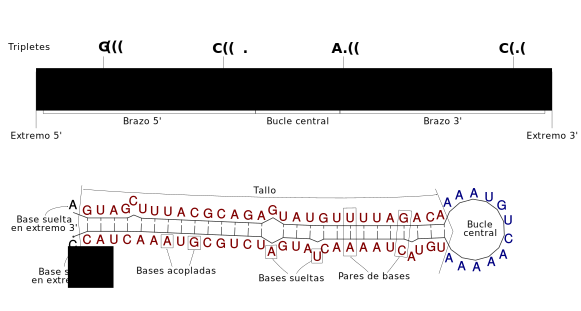
\includegraphics[width=\textwidth]{figures/triplet/triplete.pdf}

\caption{\captionStyle\protect\label{triplet}
Ejemplo de extracción de características de tripletes para el
\premirna{} \dset{cel-lsy-6}\footnotemark.
}
\end{figure}
%
El cálculo de las \caract{s} de tripletes requiere que el ejemplo
tenga una estructura secundaria con forma de horquilla, con un único
bucle central.
De otro modo, la definición del ``tallo'' pierde sentido y el
algoritmo falla, retornando valores nulos para estas \caract{s} e
invalidando cualquier procesamiento posterior del ejemplo en cuestión.
Por ello, los grupos de \caract{s} de tripletes \dset{T} y \dset{X} no
son aptos para un uso general, sino que deberán utilizarse sólo cuando
se garantice la estructura secundaria forma de horquilla para todos
los ejemplos.

En la Tabla a continuación se detallan las $36$ características de
tripletes \cite{xue} y su posición en el vector de características.

\newcommand{\tripletRow}[1]{
  \stepcounter{FeatureCounter}\theFeatureCounter & $N_{\T{\mono{#1}}}$
  & Número de ocurrencias del triplete \mono{#1} en la región del
  tallo \cite{xue}.
  }

\begin{longtable}{@{}p{0.07\textwidth}%
@{\hspace{0.01\textwidth}}p{0.17\textwidth}%
@{\hspace{0.01\textwidth}}p{0.74\textwidth}@{}}
  \headRow\endhead
  \tripletRow{A...}\\
  \tripletRow{A..(}\\
  \tripletRow{A.(.}\\
  \tripletRow{A.((}\\
  \tripletRow{A(..}\\
  \tripletRow{A(.(}\\
  \tripletRow{A((.}\\
  \tripletRow{A(((}\\
  \tripletRow{G...}\\
  \tripletRow{G..(}\\
  \tripletRow{G.(.}\\
  \tripletRow{G.((}\\
  \tripletRow{G(..}\\
  \tripletRow{G(.(}\\
  \tripletRow{G((.}\\
  \tripletRow{G(((}\\
  \tripletRow{C...}\\
  \tripletRow{C..(}\\
  \tripletRow{C.(.}\\
  \tripletRow{C.((}\\
  \tripletRow{C(..}\\
  \tripletRow{C(.(}\\
  \tripletRow{C((.}\\
  \tripletRow{C(((}\\
  \tripletRow{U...}\\
  \tripletRow{U..(}\\
  \tripletRow{U.(.}\\
  \tripletRow{U.((}\\
  \tripletRow{U(..}\\
  \tripletRow{U(.(}\\
  \tripletRow{U((.}\\
  \tripletRow{U(((}\\
  33 & $L_3$ &
  Longitud del tallo: cantidad de nucleótidos en el tallo de
  la estructura de horquilla \cite{xue}. \\
  34 & $P$ &
  Número de pares de bases en el pre-miRNA \cite{xue}. \\
  35 & $L_3/P$ &
  Grado de complementariedad entre los dos brazos de la estructura de
  horquilla: para una complementariedad perfecta, se da el valor
  mínimo 2. Este valor aumenta conforme aumenta el número de
  bases ``sueltas'' (no acopladas) en el tallo \cite{xue}. \\
  36 & $GC=\frac{N_\ntC+N_\ntG}{L_3}$ &
  Proporción de bases \ntG y \ntC en el tallo.  Se calcula contando el
  número de bases \ntC y \ntG en el tallo y dividiendo por $L_3$
  \cite{xue}.
\end{longtable}

%
%
\subsubsection{Características de la secuencia}
%
Las \caract{s} de la secuencia se proponen en los trabajos \e{miPred}
\cite{ng} y \e{microPred} \cite{batuwita}.
Se calculan directamente a partir de la cadena de texto que representa
la secuencia, ignorando las propiedades de la estructura secundaria.
Se incluyen medidas que cuentan la longitud de la secuencia, el número
de ocurrencias de las bases \ntA{}, \ntG{}, \ntC{} y \ntU{} en forma individual
y en combinaciones de dos posiciones consecutivas (dinucleótidos).
En la Tabla a continuación se enumeran las $23$ \caract{s} de la
secuencia \cite{ng,batuwita} según la posición que ocupan en el vector
de \caract{s}.

\newcommand{\dnRow}[1]{
  \stepcounter{FeatureCounter}\theFeatureCounter
  & $N_{\T{\mono{#1}}}$
  & Número de dinucleótidos \mono{#1}.}
%
\setcounter{FeatureCounter}{43}
%
\begin{longtable}{@{}p{0.07\textwidth}%
@{\hspace{0.01\textwidth}}p{0.13\textwidth}%
@{\hspace{0.01\textwidth}}p{0.78\textwidth}@{}}
  \headRow\endhead
  37 & $L$ &
  Longitud de la secuencia. \\
  38 & $N_\ntA{}$ &
  Número de nucleótidos \ntA{}. \\
  39 & $N_\ntC{}$ &
  Número de nucleótidos \ntC{}. \\
  40 & $N_\ntG{}$ &
  Número de nucleótidos \ntG{}. \\
  41 & $N_\ntU{}$ &
  Número de nucleótidos \ntU{}. \\
  42 & $N_\ntC{}+N_\ntG{}$ &
  Número de nucleótidos \ntC{} y \ntG{}. \\
  43 & $N_\ntA{}+N_\ntU{}$ &
  Número de nucleótidos \ntA{} y \ntU{}. \\
  \dnRow{AA}\\
  \dnRow{AC}\\
  \dnRow{AG}\\
  \dnRow{AU}\\
  \dnRow{CA}\\
  \dnRow{CC}\\
  \dnRow{CG}\\
  \dnRow{CU}\\
  \dnRow{GA}\\
  \dnRow{GC}\\
  \dnRow{GG}\\
  \dnRow{GU}\\
  \dnRow{UA}\\
  \dnRow{UC}\\
  \dnRow{UG}\\
  \dnRow{UU}\\
\end{longtable}

%
%
\subsubsection{Características de la estructura secundaria}
%
Al igual que las medidas de la secuencia, este grupo de \caract{s} se
basa en aquellas \caract{s} propuestas en los trabajos \e{miPred}
\cite{ng} y \e{microPred} \cite{batuwita}.
Consiste en $7$ medidas derivadas de la estructura secundaria, tales
como la ocurrencia de diferentes tipos de pares de bases (bases
acopladas) \bp{A}{U}, \bp{G}{C}, y \bp{G}{U}, y medidas basadas en un
valor denominado \e{Mínima Energía Libre}, que resulta del algoritmo
de plegado (predicción de la estructura secundaria).
A continuación, se listan las $7$ \caract{s} según la posición que
ocupan dentro del vector.

\begin{longtable}{@{}p{0.07\textwidth}%
@{\hspace{0.01\textwidth}}p{0.07\textwidth}%
@{\hspace{0.01\textwidth}}p{0.13\textwidth}%
@{\hspace{0.01\textwidth}}p{0.70\textwidth}@{}}
  \headRow\endhead
  60 & \dset{E} & MFE &
  Mínima energía libre. \\
  61 & \dset{E} & MFEI$_1$ &
  MFEI$_1=\frac{\T{MFE}}{100\cdot(N_\ntC{}+N_\ntG{})}$. \\
  62 & \dset{E} & MFEI$_4$ &
  MFEI$_4=\T{MFE}/P$. \\
  63 & \dset{E} & $dP = P/L$ &
  Número de pares de bases dividido entre la longitud total $L$. \\
  64 & \dset{E} & $P_{\bp{A}{U}}/L$ &
  Número de pares \bp{A}{U} normalizado. \\
  65 & \dset{E} & $P_{\bp{G}{C}}/L$ &
  Número de pares \bp{G}{C} normalizado. \\
  66 & \dset{E} & $P_{\bp{G}{U}}/L$ &
  Número de pares \bp{G}{U} normalizado.
\end{longtable}

%
%
%
\subsection{Normalización de los vectores de características}
%
Las \caract{s} que componen el vector de \caract{s} poseen rangos
numéricos diferentes, ya que representan cantidades de naturaleza
diversa.
Esto implica que algunos componentes del vector de \caract{s} tendrán
magnitudes mayores que otros, generando una ponderación implícita de
algunas \caract{s} por sobre otras.
La normalización permite evitar este problema modificando el rango de
cada \caract{} a un intervalo preestablecido, típicamente $[0,1]$ o
$[-1,+1]$.
Esto deriva en problemas mejor condicionados desde el punto de vista
numérico e incrementa la velocidad de convergencia en el
entrenamiento \cite{nnfaq2}.

Dado un vector de características $\xx=(x_{1},x_{2},\ldots,x_{F})$, la
versión normalizada $\xx^*$ del mismo vector se calcula según
%
\begin{align}
  \label{e3:norm-op}
  x_j^{*} = ( x_j + d_j ) s_j, \quad j=1,\ldots,F,
\end{align}
%
donde $\B{s}$ es un \e{vector de escala} y $\B{d}$ es un \e{vector de
  desplazamiento} que permiten transformar las componentes $x_j$ al
intervalo especificado.

Cuando el objetivo es la generación de un modelo de clasificador, los
vectores $\B{s}$ y $\B{d}$ se calculan con el primer archivo leído a
la entrada del método.
El primer paso es armar una matriz
$M{}_{({N}\times{}F)}$, donde cada fila $i=1,\ldots,N$ corresponde a
un ejemplo y cada columna $j=1,\ldots,\F$ representa una variable
(\caract{}).
Para cada columna $j$ de $M$, se calculan los valores $d_j$ y $s_j$
que transforman el rango de la variable $x_j$ al intervalo deseado.
Para llevar las variables al rango $[0,1]$, $d_j$ y $s_j$ se
calculan según
%
\begin{align}
  d_j &= - \min_i m_{ij}, &
  s_j &= \frac{1}{\max_i m_{ij} - \min_i m_{ij}}.
\end{align}
%
Similarmente, para llevar las variables al intervalo simétrico
$[-1,+1]$,
%
\begin{align}
  d_j &= -\frac{1}{2}\left(\max_i m_{ij} + \min_i m_{ij}\right), &
  s_j &= \frac{2}{\max_i m_{ij} - \min_i m_{ij}}.
\end{align}
%
Una vez calculados los vectores $\B{d}$ y $\B{s}$, se aplica la
normalización (\iflatexml{}Ecuación~\ref{e3:norm-op}\else\autoref{e3:norm-op}\fi)
sobre todos los ejemplos leídos en la entrada.

Para un modelo de clasificador entrenado con datos normalizados, es
importante aplicar la misma normalización sobre todos los ejemplos
futuros a clasificar.
Por ello, los vectores $\B{d}$ y $\B{s}$ se guardan como parte del
mismo modelo.
Cuando se provee un modelo como entrada al método, los ejemplos se
normalizan según la información contenida en el mismo.

%
%
%
\subsection{Partición de los datos}
%
La partición de los datos implementa el método de retención, separando
los conjuntos de datos en un conjunto \e{de entrenamiento} y otro
\e{de prueba}, a partir de la especificación del usuario al momento de
la carga de los archivos.

Internamente, los conjuntos de datos de entrenamiento y prueba se
guardan como matrices $M^E$, $M^P$, de 70 columnas y $\ell^E$ y
$\ell^P$ filas, respectivamente.
Las primeras 66 columnas representan los vectores de características
normalizados de cada ejemplo. La columna 67 contiene la clase del
ejemplo cuando es conocida. Las restantes 3 columnas contienen índices
de referencia, para lograr trazabilidad de los ejemplos.

Para cada conjunto de datos $D_n$ de $\ell_n$ elementos,
correspondiente a un archivo leído en la entrada, se arma una matriz
provisoria con los vectores de \caract{s} correspondientes a cada
ejemplo y se agrega la información de clase y los índices en las
últimas 4 columnas. Luego, se intercambian las filas en forma
pseudoaleatoria, para finalmente seleccionar las primeras
$\ell_n\cdot{}p_n^E$ filas de la matriz resultante, agregándolas al
conjunto de entrenamiento, y las $\ell_n\cdot{}p_n^P$ filas
subsiguientes al conjunto de prueba. Los valores
$0\leq{}p_n^E,p_n^P\leq1$ son especificados por el usuario e indican
la proporción de elementos del conjunto a utilizar para entrenamiento
y prueba, respectivamente.

Una vez incorporados todos los archivos en los conjuntos de
entrenamiento y prueba, se permutan sus filas en forma
pseudoaleatoria. De este modo, quedan conformados el conjunto de
entrenamiento, utilizado en la obtención del modelo, y el conjunto de
prueba, utilizado para clasificación de nuevos ejemplos.

%% Una vez efectuadas la extracción de características y la
%% normalización, los archivos de entrada originales se han convertido en
%% conjuntos $D_1,\ldots,D_N$ que contienen los vectores de
%% características normalizados y la información de clase para cada
%% ejemplo. La partición de los datos refiere al armado de los conjuntos
%% de entrenamiento $D^E$ y prueba $D^P$ con los elementos de estos
%% conjuntos a partir de la especificación del usuaio.

%% El conjunto $D_n=((\xx_i,y_i)),\,i=1,\ldots,\ell_n$ se corresponde con
%% el $n$-ésimo archivo de entrada. El objetivo es armar los conjuntos de
%% entrenamiento $D^E$ y de prueba $D^P$ con elementos de los
%% $D_n,\,n=1,\ldots,N$.  Para cada conjunto $D_n$, el usuario especifica
%% una proporción $p_n^E$ de elementos del conjunto $D_n$ a utilizar como
%% entrenamiento, y otra proporción $p_n^P$ de elementos de $D_n$ a
%% utilizar para prueba. Los valores de $p_n^E,p_n^P$ son tales que
%% %
%% \begin{align}
%%   0\ \leq\ p_n^E, p_n^P\ \leq\  p_n^E + p_n^P\ \leq\ 1,
%% \end{align}
%% %
%% esto es, $p_n^E$ y $p_n^P$ son números enre 0 y 1 cuya suma es menor o
%% igual a 1.

%% El primer paso consiste en permutar aleatoriamente el orden de los
%% elementos de los conjuntos de entrada $D_n$
%% %
%% \begin{align}
%%   D^*_n = ((\xx_j,y_j)), \quad j = \sigma(i,\ell_n,s), \quad i=1,\ldots,\ell_n,
%% \end{align}
%% %
%% donde $\sigma$ es una función de permutación pseudoaleatoria que
%% requiere la especificación de una \e{semilla} $s$. Seguidamente se
%% particiona cada conjunto $D_n$ en sub-conjuntos de entrenamiento
%% y prueba
%% %
%% \begin{align}
%%   D^E_n &= ((\xx_u,y_u)\in D^*_n),& u&=1,\ldots,\ell^E_n, \\
%%   D^P_n &= ((\xx_v,y_v)\in D^*_n),& v&=1,\ldots,\ell^P_n,
%% \end{align}
%% %
%% donde
%% %
%% \begin{align}
%%   \begin{split}
%%     \ell^E_n &= \left\lfloor\ell_n\cdot p_n^E \right\rceil, \\
%%     \ell^P_n &= \lfloor\ell_n\cdot p_n^P\rceil.
%%   \end{split}
%% \end{align}
%% %
%% El operador $\lfloor\cdot\rceil$ es el operador de redondeo.
%% Finalmente, se ensamblan los conjuntos de entrenamiento y prueba según
%% %
%% \begin{align}
%%   D^E &= \left( (\xx_u,y_u) \in \bigcup_n {D}^E_n \right), &
%%   u &= \sigma(i,\ell^E,s), &
%%   i &= 1,\ldots,\ell^E, &
%%   \ell^E &= \left| D^E \right| = \sum_n \ell^E_n ,\\
%%   D^P &= \left( (\xx_v,y_v) \in \bigcup_n {D}^P_n \right), &
%%   v &= \sigma(j,\ell^P,s), &
%%   j &= 1,\ldots,\ell^P, &
%%   \ell^P &= \left| D^P \right| = \sum_n \ell^P_n .
%% \end{align}
%% %
%% Esto es, los conjuntos de entrenamiento $D^E$ y prueba $D^P$ se arman
%% concatenando los respectivos $D^E_n$ y $D^P_n$ y luego permutando
%% aleatoriamente el orden de los ejemplos en los conjuntos resultantes.

%
%
\subsubsection{Generación de particiones para validación cruzada}
%
%La generación de las particiones de validación cruzada se lleva a cabo
%una vez armado el conjunto de entrenamiento con $\ell^E$ elementos.
Las particiones de validación cruzada se generan como un conjunto de
índices sobre el conjunto de entrenamiento.
En primer lugar, se genera un vector de índices en orden aleatorio
entre $1$ y $\ell^E$, el número de ejemplos en el conjunto de
entrenamiento.
Luego, se seleccionan los primeros $p\cdot\ell^E$ elementos para la
partición de validación, y los elementos restantes para la partición
de estimación correspondiente.
La operación se repite para cada $j=1,\ldots,k$, efectuando un
desplazamiento circular del vector de índices en $\ell^E/k$ elementos
entre iteraciones.
El parámetro $p$ regula la proporción de elementos de entrenamiento a
utilizar para validación, mientras que $k$ determina el número de
iteraciones de la validación cruzada.
Ambos parámetros pueden ser especificados por el usuario, y por
defecto se utilizan los valores $k=10$ y $p=1/k$, siguiendo el ejemplo
de la función de Matlab \func{crossval}\footnote{%
  La documentación de la función \func{crossval} puede encontrarse en
  \url{https://www.mathworks.com/help/stats/crossval.html}
}, y tal como se recomienda en \cite{hastie}.
Cuando $p=1/k$, cada ejemplo del conjunto de entrenamiento será
utilizado exactamente una vez para validación.

%
%
%
\section{Construcción del modelo del clasificador MLP}
%
La tarea de generación del modelo MLP se efectúa en dos pasos.  En
primer lugar, se determina el número óptimo de neuronas en la capa
oculta mediante una estrategia de búsqueda exhaustiva o trivial,
buscando maximizar la tasa de clasificación sobre un conjunto de
validación cruzada.

Luego se procede a efectuar el entrenamiento propiamente dicho, con
regularización de corte prematuro cuando el error de validación
cruzada alcanza su valor mínimo.

La arquitectura de la red resultante contendrá una o ninguna capa
oculta.

En todo entrenamiento del clasificador, se promedian en realidad cinco
redes inicializadas aleatoriamente, y la salida del clasificador en
realidad es un voto mayoritario de la salida de estas cinco redes.

Adicionalmente, se acepta el valor especial de 0 neuronas ocultas para
representar un MLP sin capa oculta, capaz de efectuar clasificación lineal.

Las estrategias de selección del \hparam{} de la red (el número de
neuronas en la capa oculta) son
%
\begin{description}
\item[Estrategia trivial:] Consiste en seleccionar cero neuronas
  en la capa oculta, sin entrenamiento. Esto redunda en una red que es
  capaz de efectuar separación lineal, y se utiliza como criterio de base para
  establecer el rendimiento de la red.
\item[Estrategia de búsqueda exhausiva:] Consiste en determinar, mediante prueba y error,
  el número óptimo de neuronas que maximizan una tasa promedio de validación cruzada.
\end{description}
%
Una vez encontrado el valor óptimo, se procede al entrenamiento.

%
\subsection{Estrategia trivial}
%
Tal como su nombre lo indica, esta estrategia es la más básica para
determinar el número de neuronas en la capa oculta.
Consiste simplemente en devolver siempre el valor $0$ como cantidad
``óptima'' de neuronas en la capa oculta, sin efectuar entrenamiento
alguno.
El modelo resultante al utilizar esta estrategia es equivalente a un
perceptrón simple, y funciona como un clasificador lineal.
Si bien esta estrategia no efectúa optimización alguna, resulta útil
para generar un modelo ``base'' para comparar el rendimiento frente a
otros modelos generados con una estrategia más compleja.

%
\subsubsection{Búsqueda exhaustiva}
%
La estrategia de búsqueda exhaustiva utiliza como función objetivo el
valor $G_m$ promedio de validación cruzada, y selecciona los
hiperparámetros óptimos mediante prueba y error dentro de un rango
preestablecido. Dado que la naturaleza de los hiperparámetros es
diferente según el clasificador, el algoritmo de búsqueda también
difiere en cada caso.

El hiperparámetro del perceptrón multicapa es el número de neuronas en
la capa oculta $h$, una variable discreta no negativa. La
inicialización aleatoria del perceptrón multicapa introduce
fluctuaciones aleatorias en la función objetivo $G_m$ de validación
cruzada, lo que implica que se deben efectuar una gran cantidad de
repeticiones de inicialización--entrenamiento--prueba para obtener
resultados fiables.  Por ello, en lugar de efectuar la búsqueda sobre
todos los valores posibles, se prueban 20 valores de $h$ entre 0 y 200
en una escala aproximadamente logarítmica:
%
\begin{align}
  \label{mlp-hidden-tries}
  h=0,1,2,3,4,5,7,9,11,14,19,24,32,41,54,70,91,118,154,200.
\end{align}
%
Por defecto, se efectúan 5 repeticiones de
inicialización--entrenamiento--prueba para cada valor de $h$. Se
selecciona aquel valor de $h$ para el cual se obtuvo el mayor valor de
$G_m$ de validación cruzada en promedio.

%
\subsection{Entrenamiento}
%
Una vez determinado el número óptimo de neuronas en la capa oculta,
se inicializa aleatoriamente una red MLP con la topología especificada.
Por defecto, el entrenamiento se efectúa mediante el método de
retropropagación Rprop, utilizando las rutinas propias de Matlab.
La regularización del entrenamiento se efectúa separando un 20\% de
los ejemplos, y deteniendo el entrenamiento cuando el error de
clasificación sobre estos ejemplos alcanza su valor mínimo.

La inicialización aleatoria del perceptrón multicapa condiciona el
algoritmo de retropropagación, lo que en algunos casos deriva en
soluciones subóptimas.
Para contrarrestar este efecto, se soporta el entrenamiento de
múltiples redes MLP en paralelo con inicializaciones aleatorias
diferentes.
En este caso, el modelo obtenido es en realidad un arreglo de modelos:
para obtener predicciones de clase, la salida global se determina a
partir de la \e{moda} de las salidas de los modelos contenidos en el
arreglo.

%
%
\section{Construcción del modelo del clasificador SVM}
%
AL igual que para el caso del clasificador MLP, la construcción
del modelo SVM es un proceso de dos etapas: en primer lugar se determinan
valores óptimos para los hiperparámetros, y una vez encontrados, se procede a
entrenar el modelo ``hiperparametrizado''.

A diferencia del caso MLP, sin embargo, en una máquina de vectores de soporte
los \hparam{s} pueden ser más de uno, y se trata de variables continuas.

Esto junto a las propiedades analíticas de la SVM permite aplicar estrategias
de selección de hiperparámetros más complejas que aprovechan mejor la información
del modelo SVM. Incluso, se puede aplicar optimización mediante descenso por gradiente.
%
\begin{description}
\item[Estrategia trivial:] Consiste en seleccionar hiperparámetros
  preestablecidos, sin entrenamiento. Se utiliza como estrategia
  ``básica'' para comparación de los métodos.
\item[Estrategia de búsqueda en la grilla:] Efectúa una búsqueda
  exhaustiva de los hiperparámetros maximizando la tasa de
  clasificación de validación cruzada.
\item[Estrategia de minimización del error empírico:] Realiza una
  búsqueda por gradiente en el espacio de los hiperparámetros de la
  tasa de clasificación de validación cruzada.
\item[Estrategia de minimización de la cota RMB]: Minimiza una función de derivación teórica
  intentando maximizar la tasa de clasificación.
\end{description}
%

%
%
\subsection{Selección trivial}
%
La estrategia de selección trivial consiste en seleccionar valores
preestablecidos (genéricos) para los hiperparámetros, apropiados para
la mayoría de los problemas.

La estrategia selecciona el valor $1$ para el hiperparámetro de
regularización $C$ \cite{libsvm}, y un valor $\gamma=\frac{1}{2F}$
para el hiperparámetro de amplitud del núcleo RBF, donde $F$ es el
número de características consideradas \cite{glasmachersigel}.

Es de esperar que el modelo resultante del uso de esta estrategia no
sea óptimo, aunque sí será de utilidad para la comparación con otros
modelos obtenidos mediante estrategias más avanzadas.

%
%
\subsection{Búsqueda en la grilla}
%
La \e{búsqueda en la grilla} propuesta en \cite{hsu}, permite
optimizar los hiperparámetros de regularización $C$ y $\gamma$ cuando
se utiliza un núcleo RBF.
La idea general de esta estrategia es considerar cada combinación de
hiperparámetros $(C,\gamma)$ como puntos en el plano $C\gamma$.
Comenzando por una serie de puntos espaciados regularmente
en espacio logarítmico $(\log C,\log\gamma)$, que determinan la
``grilla'' inicial, se entrena y evalúa el clasificador sobre cada
punto (cada combinación de hiperparámetros), para luego interpolar
(``refinar la grilla'') en las cercanías de los puntos donde se
obtiene la mayor tasa de clacificación $G_m$.
La búsqueda continúa repitiendo el procedimiento sobre los puntos no
evaluados hasta satisfacer un criterio de corte.

La grilla inicial viene dada por combinaciones de los siguientes
puntos de muestreo para los hiperparámetros
%
\begin{align}
  \label{initial-grid}
  \log_2 C     \tab= -5, -3, -1, 1, \ldots, 15, \tabs
  \log_2\gamma \tab= -15,-13, -11, \ldots, 3.
\end{align}
%
Para cada punto $(C_i,\gamma_j)$, se entrena y prueba el clasificador
SVM, obteniendo un ${G_m}_{ij}$ promedio de validación cruzada.

En etapas sucesivas, se interpola la grilla alrededor de los puntos
donde se obtuvieron los mejores valores $G_m$. Se definen tres
algoritmos heurísticos que determinan cuáles puntos interpolar:
%
\begin{itemize}
\item
  \e{Zoom}: En un primer paso, se convoluciona la grilla con una
  ventana cuadrada uniforme de valor unitario, obteniendo una versión
  ``suavizada'' de la grilla. Se interpolan puntos en una región
  cuadrada centrada en el punto con mayor valor $G_m$ ``suavizado''.
\item
  \e{Umbral}: A partir de un umbral $G_m$ definido por el usuario,
  por defecto el percentil 90, se interpola en cada dimensión
  alrededor de los puntos por encima del umbral.
\item
  \e{$n$-mejores}: Similar al umbral, se seleccionan $n$ puntos
  con los mayores valores de $G_m$. Se interpola la grilla en ambas
  dimensiones alrededor de estos puntos.
\end{itemize}
%
Una vez interpolada la grilla, se calcula el valor $G_m$ promedio de
validación cruzada para los puntos interpolados. El procedimiento de
refinamiento se repite hasta un máximo de $N$ iteraciones o hasta
satisfacer un criterio de corte.

La búsqueda en la grilla tiene la ventaja de ser conceptualmente
simple, sin embargo, se torna inviable cuando el vector de parámetros
$\B{\theta}$ contiene más de 2 elementos.
Dado que se trata de un método de búsqueda exhaustiva, resulta
generalmente lento.
Cuando se trabaja con un clasificador SVM con núcleo lineal, la grilla
tiene una única dimensión: la del hiperparámetro $\log C$.

%
%
\subsection{Criterio del error empírico}
%
El \e{criterio del error empírico} es una estrategia de selección de
\hparam{s} basada en la propuesta presentada en \cite{ayat}, que
optimiza los \hparam{s} del clasificador minimizando una función
objetivo denominada \e{error empírico}\,\footnote{
  El lector experto encontrará ambigua la denominación de la función
  ``error empírico'', ya que en la disciplina este nombre se utiliza
  como equivalente de ``error de entrenamiento''.
  En este trabajo, se mantiene la denominación de los autores
  \cite{ayat}, definiendo ``error empírico'' como la función que
  calcula un error probabilístico de validación cruzada sobre el
  conjunto de entrenamiento.
}.
Esta función mide el error de validación cruzada sobre el conjunto de
entrenamiento acoplando un modelo probabilístico a la salida del
clasificador, y permite su optimización mediante descenso por
gradiente ya que sus derivadas respecto de los \hparam{s} son
calculables.

En la propuesta original \cite{ayat}, la función {error empírico} se
optimiza únicamente respecto a los \hparam{s} del núcleo.
En la estrategia implementada, se agregó soporte para la optimización
del hiperparámetro $C$, siguiendo el método del cálculo de la derivada
respecto de $C$ propuesto en \cite{keerthi} y \cite{glasmachers}, tal
como se implementa en \cite{shark}.

%
\subsubsection{La función error empírico}
%
El error de validación del modelo $h$ sobre un conjunto
$V=((\xx_j,y_j))\,i=1,\ldots,\ell^V$ puede escribirse
%
\begin{align}
\label{e3:error-test-alt}
  E^V &= \frac{1}{\ell^V}\sum_{j=1}^{\ell^V} H(-{y}_j {h}(\xx_j))
\end{align}
%
donde $H(\cdot)$ es la función escalón de Heaviside. Esta formulación
del error con la función escalón $H$ en lugar de la pérdida $0-1$
equivalente pone de relieve el hecho que el error $E^V$ es una función
discontinua, al ser suma de discontinuas, y por tanto no derivable.
La función ``error empírico'' \cite{ayat} se construye a partir de una
interpretación bayesiana del concepto de error, y posee las
características deseables de continuidad y derivabilidad que permiten
su utilización como función objetivo en un esquema de minimización por
descenso por gradiente.

Si se conoce la \e{probabilidad a posteriori} $p_j$ de que el ejemplo
$\xx_j$ pertenezca a la clase positiva
%
\begin{align}
  \label{e3:pk}
  p_j = p(\xx_j) = P(h(\xx_j)=+1|\xx_j),
\end{align}
%
se puede caracterizar la \e{probabilidad de error} $E_j$ cometido al
clasificar el ejemplo $\xx_j$ según
%
\begin{align}
\label{e3:Ek}
  E_j = P(h(\xx_j)\neq y_j) = |t_j-{p}_j| =
  \begin{cases}
    {p}_j, & t_j=0\\ 1-{p}_j, & t_j = 1,
  \end{cases}
\end{align}
%
donde $t_j=\frac{y_j+1}{2}$ es un ``valor deseado'' calculado a partir
de la clase conocida $y_j$. La probabilidad de error para el conjunto
completo $V$ puede escribirse
%
\begin{align}
\label{Err1}
  E = \frac{1}{\ell^V}\sum_{j=1}^{\ell^V} E_j.
\end{align}
%
Ésta es la función \e{error empírico}. Puede comprobarse que, a
diferencia del error con pérdida 0-1, ésta es una función continua y
derivable.

Para el cálculo de $E$ se requiere conocer la probabilidad $p_j$
(\iflatexml{}Ecuación~\ref{e3:pk}\else\autoref{e3:pk}\fi), la cual no
puede determinarse a partir de la salida binaria del modelo SVM.  En
su lugar, se utiliza un estimador de $\hat{p}_j$.

%
\subsubsection{Salida probabilística del modelo SVM}
%
La salida del modelo de una máquina de vectores de soporte
(\iflatexml{}Ecuación~\ref{e2:svm-model-hard}\else\autoref{e2:svm-model-hard}\fi)
puede entenderse como el resultado de aplicar la operación signo sobre
una función continua $f$:
%
\begin{align}
\label{e3:svm-model-as-sign-f}
  h(\xx) \tab= \T{signo}(f),\tabs
  f\tab=\langle\ww,\BPhi(\xx)\rangle+b.
\end{align}
%
Aplicando el método propuesto por {Platt} en \cite{platt}, se calcula
un estimador $\hat{p}$ para la probabilidad real $p=P(h=+1|\xx)$
utilizando el valor de $f$:
%
\begin{align}
\label{e3:p-hat}
  \hat{p}\tab=\frac{1}{1+e^{Af+B}} \tabs\approx\,{}p.%P(h=+1|\xx).
\end{align}
%
Los valores $A$ y $B$ se determinan a partir del conjunto de validación
$V$ resolviendo el problema de optimización
%
\begin{align}
  \arg\min_{A,B} \tabs -\sum_{j=1}^{\ell^V} t_k\log(\hat{p}_k)+(1-t_k)\log(1-\hat{p}_k),
  \label{abproblem}
\end{align}
%
en donde $\hat{p}_k$ viene dado por la
\iflatexml{}Ecuación~\ref{e3:p-hat}\else\autoref{e3:p-hat}\fi{}, y
$t_k=\frac{1}{2}({y_k+1})$.
Este problema se resuelve mediante el algoritmo de optimización
estándar BFGS \cite{nocedal}, observando que las derivadas de
$\hat{p}_k$ respecto de $A$ y $B$ vienen dadas por
%
\begin{align}
  \begin{split}
    \dpar{\hat{p}_k}{A}{}&=-f_k e^{Af_k+B}\frac{1}{(1+e^{Af_k+B})^2}
    =-f_k\hat{p}_k(1-\hat{p}_k),\\
    \dpar{\hat{p}_k}{B}{}&=    -e^{Af_k+B}\frac{1}{(1+e^{Af_k+B})^2}
    =-   \hat{p}_k(1-\hat{p}_k).
  \end{split}
\label{e3:deriv-pk-wrt-AB}
\end{align}
%
%% Utilizando estas derivadas, el cálculo de la solución al problema
%% (\ref{abproblem}) se efectúa mediante un algoritmo de descenso por
%% gradiente.

%% La elección de una función logística como $\hat{p}_k$ se basa en la
%% presunción de que las salidas $f_k$ para las entradas $\{\xx_k\}$ de
%% clase positiva tienen una distribución gaussiana en $f$.

%% Una interpretación intuitiva de $\hat{p}_k$ es que, para una salida
%% $f_k$ de gran magnitud, que se ubica lejos del hiperplano de separación
%% en el espacio inducido por el núcleo, el clasificador SVM tiene amplia
%% certeza de su decisión.  Asimismo, se tendrá que cuando el valor de
%% $f_k=0$, $x_k$ recae exactamente en el plano de separación y se
%% obtiene la peor predicción posible $\hat{p}_k=0.5$ y, similarmente,
%% cuanto más ancho sea el margen de separación, más suave deberá ser la
%% pendiente de $\hat{p}_k$.

%
\subsubsection{Cálculo del gradiente $\grad{E}$}
\label{se:gradE}
%
Para poder utilizar un método de descenso por gradiente en el espacio
de los \hparam{s} se considera un vector genérico de \hparam{s}
$\Btheta$ de modo que $E=E(\Btheta)$, y se calculan las derivadas de
$E$ respecto de los mismos.
En primer lugar, se tiene
%
\begin{align}
\label{gradE}
  \grad{E} = \sum_{k=1}^{\ell^V} \grad{E_k} =
  \sum_{ \{i:t_k=0\}  } \grad{\hat{p}_i}
  - \sum_{ \{j:t_k=1\}  } \grad{\hat{p}_j}
  = \sum_{k=1}^{\ell^V} y_k \grad{\hat{p}_k}
\end{align}
%
Por la regla de la cadena, la derivada $\grad{\hat{p}_k}$ respecto de
un hiperparámetro ${\theta_j}$ es
%
\begin{align}
  \grad{\hat{p}_k}=\dpar{\hat{p}_k}{\theta_i}{} =
  \dpar{\hat{p}_k}{f_k}{}\dpar{f_k}{\theta_i}{} =
  -A\hat{p}_k(1-\hat{p}_k)\dpar{f_k}{\theta_i}{}.
  \label{eq:deriv-pk-thetak}
\end{align}
%
Para la determinación de $\dpar{f_k}{\theta_j}{}$ se sigue el
procedimiento propuesto en \cite{keerthi,glasmachers} e implementado
en \cite{shark}. En primer lugar, se observa que $f_k$ viene dado por
%
\begin{align}
  f_k = \langle \ww,\Phi(\xx_k)\rangle+b = \sum_{i=1}^\ell \alpha_i y_i k(\xx_i,\xx_k) + b,
  \label{fk}
\end{align}
%
en donde $((\xx_i,y_i)),i=1,\ldots,\ell$ son los ejemplos del conjunto
utilizado para entrenamiento, $k(\cdot,\cdot)$ es la función
núcleo, y $(\alpha_i, b)$ son los parámetros del modelo SVM $h$.
La derivada de $f_k$ respecto de algún hiperparámetro $\theta_j$ viene
dada por
%g
\begin{align}
  \dpar{f_k}{\theta_j}{} = \sum_{i=1}^\ell y_i
  \left[\dpar{\alpha_i}{\theta_j}{} k(\xx_i,\xx_k) + \alpha_i
    \dpar{k(\xx_i,\xx_k)}{\theta_j}{} \right].
\end{align}
%
Según sea el valor de $\alpha_i$ (el multiplicador correspondiente al
vector de entrenamiento $\xx_i$), se definen los conjuntos de índices
%
\begin{align}
  \label{unbounded-sv-set}
  u &= \left\{i\in\{1,\ldots,\ell\}:0<y_i\alpha_i<C \right\}\\
  \label{bounded-sv-set}
  g &= \left\{i\in\{1,\ldots,\ell\}: y_i\alpha_i=C \right\}\\
  n &= \left\{i\in\{1,\ldots,\ell\}: \alpha_i=0 \right\}.
\end{align}
%
Mediante interpretación geométrica de la solución al problema de la
SVM, se sabe que para aquellos vectores $\xx_i$ que no son de soporte,
se cumple que $\alpha_i=0$, luego las derivadas
$\dpar{\alpha_n}{\theta_j}{}$ son nulas. Cuando
$\alpha_i=\pm{}C$, el valor de $\alpha_g$ viene limitado (en valor absoluto) por el
parámetro $C$, y las derivadas $\dpar{\alpha_g}{\theta_j}{}$ son entonces
%
\begin{align}
  \dpar{\alpha_g}{C}{} \tab= y_g, \tabs \dpar{\alpha_g}{{\theta}^K_j}{} \tab= 0.
\end{align}
%
Aquí, $\theta_j^K$ denota un hiperparámetro específico del núcleo.
Para simplificar el cálculo de las derivadas de $\alpha_u$ y $b$ se
plantea el problema en forma matricial. Sea la \e{matriz del núcleo}
%
\begin{align}
  K = \begin{pmatrix} k(\xx_1,\xx_1) & k(\xx_1,\xx_2) & \cdots & k(\xx_1,\xx_\ell)
    \\ k(\xx_2,\xx_1) & k(\xx_2,\xx_2) & \cdots & k(\xx_2,\xx_\ell) \\ \vdots &
    \vdots & \ddots & \vdots \\ k(\xx_\ell,\xx_1) & k(\xx_\ell,\xx_2) & \cdots &
    k(\xx_\ell,\xx_\ell)
  \end{pmatrix}
  =
  \begin{pmatrix}
    (K_{uu}) & (K_{ug}) & (K_{un}) \\
    (K_{gu}) & (K_{gg}) & (K_{gn}) \\
    (K_{nu}) & (K_{ng}) & (K_{nn})
  \end{pmatrix}
\end{align}
%
donde en la matriz de la derecha los elementos de $K$ han sido
reordenados en submatrices $K_{uu},K_{ug},\ldots$ según los conjuntos
de índices $u, g, n$ definidos anteriormente.  Sea la matriz
%
\begin{align}
  H=\begin{pmatrix} K_{uu} & \B{1}_u \\ \B{1}_u^T & 0
  \end{pmatrix}
\end{align}
%
con $\B{1}_u$ un vector columna de $|u|$ elementos iguales a 1,
entonces la derivada de $(\B{\alpha}_u,b)^T$ respecto del
hiperparámetro $\theta_j$ viene dada por
%
\begin{align}
  \dpar{}{\theta^K_j}{} \begin{pmatrix}\alpha_{u}\\b\end{pmatrix} &=
    -H^{-1} \left[
      \dpar{H}{\theta^K_j}{}
      \begin{pmatrix}\alpha_{u}\\b\end{pmatrix}
        +C \begin{pmatrix}\dpar{K_{gu}}{\theta^K_j}{}\\0\end{pmatrix}
          y_g
          \right], \\
  \dpar{}{C}{} \begin{pmatrix}\alpha_{u}\\b\end{pmatrix} &=
    -H^{-1} \left[
      \begin{pmatrix}{K_{gu}}\\\B{1_g^T}\end{pmatrix} y_g
      \right],
\end{align}
%
donde $\B{1}_g$ un vector columna de $|g|$ elementos iguales a 1 y
$\B{y}_g$ el vector de clases correspondientes a los elementos en
$g$. Para los detalles de este resultado se refiere al lector a
\cite{glasmachers} y \cite{keerthi}.

Una vez obtenidas las derivadas de $({\B{\alpha},b})^T$ respecto de
los hiperparámetros $\B{\theta}$, la derivada de $f$  respecto
de los mismos se calcula simplemente según
%
\begin{align}
  \dpar{f_k}{C}{} &=  \sum_{i=1}^l y_i\left[
    \dpar{\alpha_i}{C}{} k(x_i,x_k) \right]
  + \dpar{b}{C}{} ,\\
  \dpar{f_k}{\theta^K_j}{} &=  \sum_{i=1}^l y_i \left[
    \dpar{\alpha_i}{\theta^K_j}{} k(x_i,x_k) +
    \dpar{k(x_i,x_k)}{\theta^K_j}{} \alpha_i \right]
  + \dpar{b}{\theta^K_j}{}.
\end{align}
%
Reemplazando estos resultados en (\ref{eq:deriv-pk-thetak}), el cálculo
del gradiente $\nabla{}E$ (\ref{gradE}) se efectúa directamente.

%
\subsubsection{Algoritmo de optimización}
%
El algoritmo comienza la búsqueda estableciendo en $1$ el valor de
todos los \hparam{s}: $\Btheta^0=(1,1,\ldots)$.
En cada iteración $t$, se efectúan los siguientes pasos:
%
\begin{enumerate}
\item
  Aplicando validación cruzada, se entrena un modelo SVM para cada
  conjunto de estimación.
\item
  Se calculan las salidas $f_k$
  (\iflatexml{}Ecuación~\ref{fk}\else\autoref{fk}\fi) de los modelos
  para todos los ejemplos $\xx_k$ en las respectivas particiones de
  validación.
\item
  Se determinan los valores óptimos de los parámetros $A$ y $B$,
  minimizando el Problema~\ref{abproblem}, partiendo de los valores
  iniciales $A_0=1$, $B_0=0$.
\item
  Se calculan las probabilidades estimadas $\hat{p}_k$ y con ellas, el
  error empírico de cada ejemplo $E_k$ y global $E$.
\item
  Se calculan las derivadas $\dpar{E}{\theta_j}{}$.
\end{enumerate}
%
La búsqueda procede en cada punto $\Btheta^t$ evaluando la función
objetivo $E$ y determinando un nuevo punto $\Btheta^{t+1}$ a partir de
la información disponible en el gradiente $\nabla{}E^t$, mediante el
algoritmo de optimización BFGS \cite{nocedal}.

%
%
\subsection{Minimización de la cota radio-margen}
%
Una cota ``radio-margen'' es una función de derivación teórica que
sirve como límite superior al error de clasificación
\e{dejando-uno-fuera} del modelo SVM sobre el conjunto de
entrenamiento.
La primera función de este tipo fue propuesta en \cite{vapnik}
para modelos SVM con regularización $L2$ y viene dada por
% vapnik sec. 10.7, pag 441
\begin{align}
  \T{RM} = 4R^2 \|\ww\|^2.
\end{align}
%
Aquí, $R$ es el radio de la hiperesfera que contiene todos los
vectores de soporte en el espacio inducido $Z$ y $\ww$ es el vector
normal al hiperplano de separación del modelo.
Puede mostrarse que la función RM cumple la propiedad
%
\begin{align}
  E_{\T{LOO}} \leq \T{RM},
\end{align}
%
donde $E_{\T{LOO}}$ es el error de validación cruzada dejando uno
fuera.
Esta propiedad, junto al hecho de ser derivable respecto de los
\hparam{s}, convierte a RM en una función objetivo idónea en un
esquema de minimización mediante descenso por gradiente.
En \cite{chapelle} se presenta un método para selección automática de
hiperparámetros basado en esta función.
Sin embargo, su utilidad práctica es limitada, ya que
la SVM con regularización $L2$ no es muy utilizada.

En \cite{chung} se proponen formulaciones alternativas a RM,
aplicables a una formulación SVM con regularización $L1$ y núcleo
gaussiano (RBF).
En particular, se considera la función
%
\begin{align}
  \rho = \rho_R \cdot \rho_M,
\end{align}
%
donde $\rho_R$ y $\rho_M$ son, respectivamente, los factores ``radio''
y ``margen''
%
\begin{align}
  \rho_R &= R^2+\frac{1}{C}, \\
  \rho_M &= \|\ww\|^2+2C\sum\xi_i.
\end{align}
%
A diferencia de {RM}, la función $\rho$ ajusta el error $E_{\T{LOO}}$
con demasiada holgura, por lo que pierde el significado original de
representar una tasa de error.
Sin embargo, mantiene la propiedad de poseer un mínimo global cerca
del punto que minimiza la tasa de error $E_{\T{LOO}}$.

\subsubsection{Función objetivo}
La estrategia aquí propuesta utiliza una de estas cotas
alternativas, denotada $\rho$ y definida según

\begin{align}
  \rho = \rho_R \cdot \rho_M,
\end{align}
donde $\rho_R$, $\rho_M$ son los factores ``radio'' y ``margen''

\begin{align}
  \rho_R &= R^2+\frac{1}{C}, \\
  \rho_M &= \|\ww\|^2+2C\sum\xi_i.
\end{align}
A diferencia de $\T{RM}$, la función $\rho$ ajusta el valor
real de $E_{\T{LOO}}$ con demasiada holgura, con lo que su valor
pierde el significado original de representar una tasa de error. Sin
embargo, tiene la importante propiedad de poseer un mínimo global en
las cercanías de los hiperparámetros óptimos $(C,\gamma)$ que
minimizan la tasa de error $E_{\T{LOO}}$.

\subsubsection{Cálculo de $\rho$}
El valor $R^2$, necesario para el cálculo de $\rho_R$, viene dado por

\begin{align}
  R^2 = 1 - \Bbeta_*^T \KK \Bbeta_*,
\end{align}
donde $\Bbeta_*$ es la solución al problema de optimización conocido
como ``SVM de una clase'' \cite{scholkopf}

\begin{align}
\begin{split}
  \arg\min_{\Bbeta}\quad&\Bbeta^T \KK \Bbeta,\\
  \T{sujeto a}    \quad&0\leq\beta_i\leq{}1,\quad{}i=1,\ldots,\ell,\\
                       &\B{1}^T_\ell\,\Bbeta=1.
  \end{split}
  \label{svm-oneclass}
\end{align}
Aquí, $\B{1}_{\ell}$ es un vector columna con $\ell$ elementos iguales
a 1, y $\KK$ es la matriz del núcleo con elementos
$k_{ij}=k(\xx_i,\xx_j)$. La matriz $\KK$ es definida positiva siempre
que se cumpla la condición

\begin{align}
\label{cond-kmatrix-defpos}
  i\neq j \iff \xx_i\neq\xx_j,\quad \forall\,i,j\in{1,\ldots,\ell},
\end{align}
esto es, siempre que no haya ejemplos repetidos en el conjunto de
entrenamiento. Sin perder mucha generalidad, se considera que tal es
el caso, y con ello, se asegura que el problema \cite{svm-oneclass}
tiene solución única \cite{SOL-UNICA-DEFINIDA-POSITIVA}.

El valor ``margen'' $\rho_M$ es dos veces la solución al problema de
optimización de la SVM (\autoref{svm-primal-blando}).  Dada la
equivalencia primal-dual de la solución, si $\Balpha$ es solución a
la forma dual (\autoref{svmprob-dual-soft}), se tiene simplemente

\begin{align}
\label{prieqdual}
  \rho_M &= 2\left(\frac{1}{2}\|\ww\|^2+C\sum\xi_i \right)
  =2\left(\B{e}^T\Balpha-\frac{1}{2}\Balpha^T\B{Q}\Balpha\right),
\end{align}
donde $\QQ$ es la matriz con elementos $Q_{ij}=y_iy_jk(\xx_i,\xx_j)$.

%
\subsubsection{Cáclulo del gradiente $\nabla\rho$}
%
El cálculo de las derivadas de $\rho$ se basa en resultados de
análisis de perturbación de problemas de optimización, ya que tanto
$\rho_R$ como $\rho_M$ son soluciones a problemas de este tipo
\cite{chung}.
Las derivadas de $\rho_R$ respecto de los hiperparámetros $C$ y
$\gamma$ vienen dadas por
%
\begin{align}
%
  \dpar{\rho_R}{C}{} &
  = \dpar{}{C}{}\left(1-\Bbeta^T\KK\Bbeta\right)
       + \dpar{}{C}{}\left(\frac{1}{C}\right)
  = -\Bbeta^T \dpar{\KK}{C}{}\Bbeta - \frac{1}{C^2}
  = -\frac{1}{C^2}, \\[1ex]
%
  \dpar{\rho_R}{\gamma}{} &
  = \dpar{}{\gamma}{}\left(1-\Bbeta^T\KK\Bbeta)\right)
       + \dpar{}{\gamma}{}\left(\frac{1}{C}\right)
  = -\Bbeta^T \dpar{\KK}{\gamma}{}\Bbeta.
%
\end{align}
%
Para garantizar la existencia de estas derivadas, resulta necesario
reescribir las restricciones $\alpha_i\leq{}C$ del problema de la SVM
(\ref{svmprob-dual-soft}) de forma tal que las mismas no dependan del
\hparam{} $C$ \cite{chung}.
Esto se logra efectuando el cambio de variable
$\bar{\Balpha}=\Balpha/C$ en (\ref{svmprob-dual-soft}):
%
\begin{align}
\begin{split}
    \max_{\bar{\Balpha}}\quad&
    f(\bar{\Balpha}) = C^2 \left( \frac{\B{1}^T\bar{\Balpha}}{C}
    -\frac{1}{2}\bar{\Balpha}^T\QQ\bar{\Balpha}\right)\\
    \T{sujeto a}\quad & \yy^T\bar{\Balpha} = 0, \\
    & 0\leq\bar{\alpha}_i\leq 1,
    \T{ para todo } i\in {1,\ldots,\ell }.
\end{split}
\end{align}
%
Con este cambio de variable el valor de $\rho_M$ viene dado por:
%
\begin{align}
  \label{eq:rmb-alpha-equiv}
  \rho_M=2\left(\B{e}^T\Balpha-\frac{1}{2}\Balpha^T\B{Q}\Balpha\right)
  = 2C^2\left(\frac{\B{1}^T\bar{\Balpha}}{C} -
  \frac{1}{2}\bar{\Balpha}^T\QQ\bar{\Balpha}\right).
\end{align}
%

Las derivadas de $\rho_M$ respecto a los \hparam{s} $C$ y $\gamma$ se
calculan según:
%
\begin{align}
    \dpar{\rho_M}{C}{}
    &= \dpar{}{C}{}\left( 2C^2\left(\frac{\B{1}^T\bar{\Balpha}}{C} -
    \frac{1}{2}\bar{\Balpha}^T\QQ\bar{\Balpha}\right)
    \right) \nonumber\\
    &= 4C \left(\frac{\B{1}^T\bar{\Balpha}}{C} -
    \frac{1}{2}\bar{\Balpha}^T\QQ\bar{\Balpha}\right)
    - 2C^2 \left(\frac{\B{1}^T\bar{\Balpha}}{C^2} \right) \nonumber\\
    &= 2\left(\B{1}^T\bar{\Balpha}
    - C \bar{\Balpha}^T\QQ\bar{\Balpha}\right) \nonumber\\
    &= \frac{2}{C} \left(\B{1}^T\Balpha - \Balpha^T\QQ\Balpha\right),\\[1ex]
    \dpar{\rho_M}{\gamma}{}
    &= \dpar{}{\gamma}{}
    2\left(  \B{1}^T\Balpha-\frac{1}{2}\Balpha^T\QQ\Balpha \right) \nonumber\\
    &= - \Balpha^T \dpar{\QQ}{\gamma}{}\Balpha \nonumber\\
    & = - \Balpha^T \left(\yy^T \dpar{\KK}{\gamma}{}\yy\right) \Balpha.
    %% \\
    %% & = \sum_{i,j=1}^\ell \alpha_i\alpha_j y_i y_j \dpar{k(\xx_i,\xx_j)}{\gamma}{}, \\[0.2em]
\end{align}
%
Los elementos $\dpar{k_{ij}}{\gamma}{}$ de la matriz
$\dpar{\KK}{\gamma}{}$ vienen dados por
%
\begin{align}
  \dpar{k_{ij}}{\gamma}{}
  = \dpar{}{\gamma}{}k(\xx_i,\xx_j)
  = \dpar{}{\gamma}{} \left(e^{-\gamma\|\xx_i-\xx_j\|}\right)
  = -k_{ij}\|\xx_i-\xx_j\|.
\end{align}
%
Finalmente se calculan las derivadas de $\rho$ respecto de $C$ y
$\gamma$ mediante
%
\begin{align}
    \dpar{\rho}{C}{} &= \dpar{\rho_M}{C}{} \rho_R + \rho_M \dpar{\rho_R}{C}{} \nonumber\\
    &= \frac{2}{C} \left(\B{1}^T\Balpha - \Balpha^T\QQ\Balpha\right) \left( R^2 + \frac{1}{C} \right)
    - 2\left(  \B{1}^T\Balpha-\frac{1}{2}\Balpha^T\QQ\Balpha \right)
    \left( \frac{1}{C^2} \right) \label{drho-dc}, \\[1em]
    \dpar{\rho}{\gamma}{} &= \dpar{\rho_M}{\gamma}{} \rho_R + \rho_M \dpar{\rho_R}{\gamma}{}\nonumber\\
    &= \left( - \Balpha^T \left(\yy^T \dpar{\KK}{\gamma}{}\yy\right) \Balpha \right)
    \left( R^2 + \frac{1}{C} \right)
    - 2\left(  \B{1}^T\Balpha-\frac{1}{2}\Balpha^T\QQ\Balpha \right)
    \left( \Bbeta^T \dpar{\KK}{\gamma}{} \Bbeta \right), \label{drho-dgamma}
\end{align}
%
en donde los elementos de las matrices $\QQ$ y $\dpar{\KK}{\gamma}{}$
son
%
\begin{align}
  q_{ij}&=y_i y_j k(\xx_i,\xx_j)= y_i y_j e^{-\gamma\|\xx_i-\xx_j\|}, \\
  \dpar{k_{ij}}{\gamma}{}&=-k_{ij}\|\xx_i-\xx_j\| = -\|\xx_i-\xx_j\|e^{-\gamma\|\xx_i-\xx_j\|}.
\end{align}
%

%
\subsubsection{Algoritmo de optimización}
%
Partiendo de un punto inicial $(C^0,\gamma^0)$ la búsqueda procede
en cada punto $(C^k,\gamma^k)$ evaluando $\rho^k$ y determinando
un nuevo punto $(C^{k+1},\gamma^{k+1})$ en la dirección del
negativo del gradiente $\nabla\rho^k$ tal que $\rho^{k+1}<\rho^k$.
La optimización de la función $\rho$ se efectúa mediante el algoritmo
BFGS \cite{nocedal} en el espacio logarítmico de los hiperparámetros
$(\ln(C),\ln(\gamma))$.
Este cambio de coordenadas se traduce en un incremento de la
estabilidad numérica y evita tener que verificar en cada iteración la
no-negatividad de $C$ y $\gamma$.
%
\begin{align}
  \dpar{\rho}{\ln C}{}= C \dpar{\rho}{C}{}, &&
  \dpar{\rho}{\ln \gamma}{}= \gamma \dpar{\rho}{\gamma}{}
\end{align}
%
Para un conjunto de entrenamiento $D=((\xx_i,y_i),i=1,\ldots,\ell)$
cada evaluación de $\rho(\Btheta_k)$ consta de los siguientes pasos
%
\begin{enumerate}
\item Entrenar una máquina de vectores de soporte con núcleo RBF
  con hiperparámetros $\Btheta_k=(C_k,\gamma_k)$ sobre el conjunto
  de entrenamiento completo $D$
\item Calcular $\Bbeta_*$ óptimo para el problema (\ref{svm-oneclass})
\item Calcular el valor de $\rho$ como el producto de
  $\rho_M$ (\ref{rho_m}) y $\rho_r$ según (\ref{rho_r})
\item Calcular el gradiente $\nabla\rho$.
\end{enumerate}
%


%
%
\subsection{Entrenamiento}
%
Una vez determinados los \hparam{s} del clasificador mediante alguna
de las estrategias antes definidas, se entrena el modelo SVM ``final''
a partir del conjunto de entrenamiento $D$ generado en la etapa de
preprocesamiento.
El modelo entrenado incorpora toda la información necesaria para poder
clasificar nuevos ejemplos, incluyendo la información de normalización
extraída del conjunto de entrenamiento.
Esto permite además la utilización del modelo como entrada al
preprocesamiento para normalizar los nuevos ejemplos a clasificar.

%
%
%
\section{Clasificación}
%
Cuando el objetivo es obtener predicciones de clase, el método recibe
como entrada un modelo de clasificador $h$ y un conjunto de datos de
prueba $T$.
La clasificación se efectúa invocando la función apropiada para el
modelo en cuestión, pasándole como argumento el conjunto de datos de
prueba leído.
La salida es un vector ${\yy}=(\hat{y}_1,\hat{y}_2,\ldots)^T$, que
contiene las predicciones de clase $\hat{y}_i$ correspondientes a cada
ejemplo $\xx_i$ del conjunto $T$:
%
\begin{align*}
  \hat{y}_i &= h(\xx_i), & \xx_i&\in{}T.
\end{align*}
%

%
%
%
\section{Interfaz de usuario}
%
El sistema incluye una interfaz de usuario de línea de comandos de
``alto nivel'', común para los distintos tipos de clasificadores
soportados.
Esta interfaz de usuario consiste en tres funciones específicas que
permiten al usuario cargar los datos del disco, generar el modelo del
clasificador, y clasificar nuevos datos.
%
\begin{enumerate}
\item
  La función \func{problem\_gen} carga datos de entrenamiento y de
  prueba según la especificación del usuario, y retorna una estructura
  en memoria denominada ``problema'', que puede utilizarse como
  entrada a las funciones de obtención del modelo y de clasificación.
  A grandes rasgos, esta función lleva a cabo la etapa de
  preprocesamiento de los datos.
\item
  La función \func{select\_model} permite obtener el modelo del
  clasificador a partir de los datos de entrenamiento.
  Recibe como argumento un problema generado con \func{problem\_gen},
  y retorna un modelo de clasificador óptimo según las opciones
  especificadas como parámetros.
  La función ofrece la funcionalidad de construcción del modelo del
  clasificador tanto MLP como SVM, con sus respectivas estrategias de
  selección de hiperparámetros.
\item
  La función \func{problem\_classify} permite clasificar los datos de
  prueba especificados dentro de un problema generado con
  \func{problem\_gen}.
  Recibe como argumento el modelo entrenado y el problema que se desea
  clasificar, y retorna una estructura en memoria con las predicciones
  para todos los elementos incluidos en el conjunto de prueba
  definidos en el problema.
\end{enumerate}
%
Los casos de uso típicos del sistema son la generación de un modelo de
clasificador y la obtención de predicciones de clase.
Utilizando las funciones de interfaz de usuario, estas tareas pueden
efectuarse según los siguientes pasos
\begin{itemize}
\item
  Obtener un nuevo modelo de clasificador:
  %
  \begin{enumerate}
  \item
    Generar un problema de clasificación mediante la función
    \func{problem\_gen} que contenga datos de entrenamiento de clase
    positiva así como negativa.
  \item
    Entrenar un clasificador invocando a la función
    \func{select\_model}.
  \end{enumerate}
  %
\item
  Obtener predicciones de clase:
  %
  \begin{enumerate}
  \item
    Generar un problema de clasificación mediante la función
    \func{problem\_gen} que contenga datos de prueba para clasificar.
  \item
    Invocar la función \func{problem\_classify}, pasándole como
    argumentos el problema y un modelo obtenido mediante
    \func{select\_model}.
  \end{enumerate}
  %
\end{itemize}
%

%
%
\section{Web de demostración del clasificador}
%
Se generó una interfaz web de demostración utilizando la herramienta
\eng{\webdemo{}} \cite{webdemobuilder}, que interactúa con el
clasificador a través de una función codificada a tal fin.
Esta función recibe un número de argumentos fijos, que son presentados
como campos del formulario web, y luego de ser invocada retorna un
``reporte'' que se presenta al usuario.
Cuando la invocación es exitosa, el reporte contiene el modelo
generado y las predicciones de clase del conjunto de prueba (si
corresponde), y puede descargarse y utilizarse posteriormente como
modelo para clasificar nuevos datos.
Cuando se encuentran errores, el reporte informa al usuario del
problema ocurrido.

%% Los argumentos de entrada en el formulario web son:
%% %
%% \begin{enumerate}
%% \item Tipo de clasificador requerido
%% \item Grupos de \caract{s} a incluir
%% \item Estrategia de selección de \hparam{s}
%% \item Archivo con datos de entrenamiento de clase positiva
%% \item Archivo con datos de entrenamiento de clase negativa
%% \item Modelo generado previamente
%% \item Archivo con datos de prueba
%% \item Clase de los datos de prueba (usado para estadísticas)
%% \end{enumerate}
%% %
Según la tarea que desee efectuar, el usuario debe cargar/seleccionar
los siguientes datos en el formulario web:
%
\begin{itemize}
\item
  {Para la generación del modelo del clasificador}:
  %
  \begin{itemize}
  \item
    Tipo de clasificador
  \item
    Conjunto de características
  \item
    Estrategia de selección de \hparam{s}
  \item
    Archivo FASTA con datos de entrenamiento de clase positiva
  \item
    Archivo FASTA con datos de entrenamiento de clase negativa
  \end{itemize}
  %
\item
  {Para efectuar clasificación con un modelo generado previamente}:
  %
  \begin{itemize}
  \item
    Archivo con el modelo de clasificador
  \item
    Archivo FASTA con datos de prueba
  \item
    Clase de los datos de prueba: opcional, utilizado para calcular
    una tasa de error sobre el conjunto.
  \end{itemize}
  %
\end{itemize}
%
Luego de la ejecución, se muestra en pantalla un enlace al archivo de
reporte, que puede ser descargado y almacenado para su utilización
posterior.

%
%\subsection{Publicación de la interfaz web de demostración}
%
\paragraph{Puesta en servicio de la demostración web}
\pdfcomment[color=Orange,open=true]{
  La idea es describir aquí la puesta en servicio de la web-demo.
}

%
%
\section{Documentación}
%
Se redactó una una guía del usuario que detalla las instrucciones de
instalación, los requerimientos del sistema, la utilización de la
interfaz de línea de comandos, y la generación y utilización de la
interfaz web.
La guía del usuario puede consultarse en el
\iflatexml{}Anexo~\ref{guiausuario}\else\autoref{guiausuario}\fi de
este documento.

Además de la guía de usuario, se incorporaron unas 700 líneas de
documentación en el código fuente siguiendo el estándar de
documentación de Matlab, lo que permite su consulta en línea mediante
la función nativa \func{help}.

%
%
%
%
\setcounter{chapter}{3}
%
\chapter{Pruebas}
%
El método desarrollado se evaluó mediante casos de prueba
experimentales basados en la bibliografía.
Cada caso, llamado \e{problema}, determina un conjunto de
entrenamiento y un conjunto de prueba, que en los experimentos se
utilizan respectivamente para generar el modelo del clasificador y
para evaluar su desempeño.
La evaluación de cada modelo se efectuó mediante las medidas de
sensibilidad (\SE), especificidad (\SP) y media geométrica de la
sensibilidad y la especificidad (\GM).
Se probaron las diferentes variantes de los clasificadores,
estrategias de selección de \hparam{s} y conjuntos de \caract{s},
tabulando los resultados obtenidos para cada combinación.
Adicionalmente, se efectuaron pruebas menos exhaustivas con problemas
``complementarios'', que brindan una idea del funcionamiento ante
tipos de problemas comunes.

En adelante, se describe la composición de los problemas y la
configuración de las pruebas, seguida de un análisis de los resultados
obtenidos con los diferentes clasificadores.
Al final del Capítulo, se presentan los resultados de las pruebas
efectuadas con los problemas complementarios.

%
%
%
\section{Descripción de los problemas}
%
Tomando como base los trabajos \cite{xue,ng,batuwita}, se definieron
tres problemas principales a partir de los conjuntos de datos
utilizados respectivamente en las pruebas de los métodos
\work{\tripletsvm}, \work{\mipred}, y \work{\micropred}.
Los problemas se denominaron \prob\tripletsvm{}, \prob{\mipred} y
\prob\micropred{}, según el nombre del trabajo en el cual se basan.

Los tres problemas contienen \premirna{s} de la especie humana
extraídos de la base de datos \dset\mirbase{} como ejemplos de clase
positiva.
\dset{\mirbase} es un repositorio de referencia en línea que contiene
ejemplos de \premirna{s} experimentalmente validados, publicado y
actualizado por el laboratorio Griffiths-Jones de la Universidad de
Manchester, Reino Unido \cite{mirbase1, mirbase2, mirbase3}.
Diferentes versiones de \work\mirbase{} se publican regularmente, con
los nuevos \premirna{s} descubiertos para diferentes organismos.
Asimismo, los ejemplos de clase negativa de los tres problemas
provienen principalmente de la base de datos \dset{coding}, un
conjunto de datos artificial creado por los autores de
\work{\tripletsvm} que contiene $8494$ ejemplos de clase negativa
llamados ``pseudo \premirna{s}'' \cite{xue}.
Estos ejemplos, generados con fragmentos del genoma humano extraídos
de regiones genómicas en las que no se ha reportado la presencia de
ningún \premirna{}, presentan una estructura secundaria con forma de
horquilla, similar a la de los \premirna{s} reales.

%
%
\subsection{Problema \tripletsvm}
%
El problema \prob{\tripletsvm} replica los datos utilizados
en \cite{xue} para la evaluación del método \work{\tripletsvm}.
Estte método fue uno de los primeros métodos de predicción de
\premirna{s} mediante Máquinas de Vectores de Soporte, y su nombre
deriva del hecho que utiliza características de tripletes como entrada
al clasificador.

Los conjuntos de entrenamiento y prueba que componen el problema
\prob{\tripletsvm} son idénticos a aquellos utilizados en \cite{xue}
para las pruebas del método \work{\tripletsvm}, ya que los autores
publicaron estos datos como material suplementario, incluyendo la
partición en entrenamiento y prueba.

Los ejemplos de clase positiva son tomados de la versión 5.0 (de
septiembre de 2004) de \work\mirbase.
De los 207 ejemplos de \premirna{s} de la especie humana (clase
positiva) presentes en esta versión, se eliminan aquellos que
contienen ramificaciones en la estructura secundaria, resultando en
193 ejemplos con estructura secundaria en forma de horquilla.
De estos ejemplos, se utilizan 163 para componer el conjunto de
entrenamiento y los 30 restantes para el conjunto de prueba.
Los ejemplos de clase negativa se obtienen de la base de datos
\dset{coding}, utilizando 168 ejemplos para el conjunto de
entrenamiento y 1000 para el armado del conjunto de prueba.

La composición de los conjuntos de entrenamiento y prueba se resume en
la \iflatexml{}Tabla~\ref{tbl:mainxue}\else\autoref{tbl:mainxue}\fi.

%
\begin{table}[h]
  \tableStyle
  \iflatexml%
  \begin{tabular}{llrcr}
  \else%
  \sisetup{
    table-format = 4.0,
  }
  \begin{tabular}{llScS}
  \fi%
    \toprule
    {Uso} & {Fuente} &{Clase}&{Especie}&{Cant. elementos}\\
    \midrule
    \mrow{2}{*}{Entrenamiento}
    & \mirbase{} 5.0 &    +1 & humana  &             163 \\
    & coding         &    -1 & humana  &             168 \\
    \midrule
    \mrow{2}{*}{Prueba}
    & \mirbase{} 5.0 &    +1 & humana  &              30 \\
    & coding         &    -1 & humana  &            1000 \\
    \bottomrule
  \end{tabular}
  \caption{\captionStyle
    Composición de los conjuntos de datos de entrenamiento y prueba
    definidos en el problema \sbs\tripletsvm{}.
  }
  \label{tbl:mainxue}
\end{table}
%

%
%
\subsection{Problema \mipred{}}
%
El problema \prob\mipred{} se basa en los datos utilizados en
\cite{ng} para el entrenamiento y prueba del método \work\mipred{}.

Si bien en \cite{ng} se describen los pasos efectuados para el armado
de los conjuntos de entrenamiento y prueba, los autores no publicaron
los datos particionados.
Esto implica que no es imposible replicar de manera exacta las pruebas
efectuadas por los autores.
En cambio, se generaron las particiones de entrenamiento y prueba
mediante selección aleatoria, mantieniendo el origen de los datos y el
número de ejemplos de clase positiva y negativa en cada caso.

Los ejemplos de clase positiva se obtuvieron de la versión $8$.$2$ (de
julio de $2006$) de la base de datos \dset{\mirbase}, mientras que los
ejemplos de clase negativa se obtuvieron de la base de datos
\dset{coding}, tal como en el problema \prob\tripletsvm{}.

Respetando el procedimiento descripto en \cite{ng}, para el armado del
conjunto de entrenamiento \dset{TR-H} se seleccionaron al azar $200$
de los $323$ ejemplos de \premirna{s} de la especie humana como clase
positiva y $400$ pseudo \premirna{s} de \dset{coding} como ejemplos de
clase negativa.
El conjunto de prueba \dset{TE-H} se compuso con los $123$ ejemplos de
clase positiva no usados para entrenamiento, y con otros $246$
ejemplos de clase negativa seleccionados al azar de la base
\dset{coding}, excluyendo aquellos ya utilizados para entrenamiento.

La composición de los conjuntos de entrenamiento y prueba de este
problema se detalla en
\iflatexml{}Tabla~\ref{tbl:pruebasng}\else\autoref{tbl:pruebasng}\fi.

%
\begin{table}[h]
  \tableStyle
  \begin{tabular}{lllScr}
    \toprule
    Nombre & Uso & Fuente &{Clase}& Especie & Cant. elementos \\
    \midrule
    \mrow{2}{*}{TR-H} & \mrow{2}{*}{Entrenamiento}
    &  \mirbase 8.2       & +1    & humana  & 200             \\
    && coding             & -1    & humana  & 400             \\
    \midrule
    \mrow{2}{*}{TE-H} & \mrow{2}{*}{Prueba}
    &  \mirbase 8.2       & +1    & humana  & 123             \\
    && coding             & -1    & humana  & 246             \\
    \bottomrule
  \end{tabular}
  \caption{\captionStyle Conjuntos de datos de entrenamiento y prueba
    definidos en el problema \sbs{\mipred}.}
  \label{tbl:pruebasng}
\end{table}
%

%
%
\subsection{Problema microPred}
%
Este problema se basa en los datos utilizados en \cite{batuwita} para
entrenamiento y prueba del método \e{microPred}.
Los ejemplos de clase positiva se obtienen de la versión 12.0 de la
base de datos \dataset{miRBase}.
Para los ejemplos de clase negativa se utilizan dos fuentes, la base
de datos \dataset{coding} y una base de datos curada por los autores,
denominada \dataset{other human ncRNAs}, que contiene en total 754
ejemplos de ncRNAs (excluyendo pre-miRNAs) de la especie humana.

En el trabajo original, los autores no especifican una separación
en conjuntos de entrenamiento y prueba, sino que utilizan todos los
ejemplos contenidos en las bases de datos positivas y negativas para
entrenamiento, y reportan las medidas de rendimiento del método
a partir de los valores obtenidos en la validación cruzada.
%% Adicionalmente, aplican sobremuestreo de la clase minoritaria (positiva)
%% mediante la técnica SMOTE \cite{smote}.
Este esquema contrasta con la forma de efectuar las pruebas en el
presente trabajo, en donde los resultados se obtienen de clasificar un
conjunto de prueba especificado y separado de los datos de entrenamiento.

El problema \micropred{} define conjuntos de entrenamiento y prueba
a partir de los datos originales del siguiente modo:
se utiliza el 85\% (587/691) de los ejemplos positivos para
entrenamiento, reservando el 15\% restante (104 ejemplos) para el
conjunto de prueba.
Tal como en el problema \sbs{miPred}, se mantiene una proporcionalidad
de 1:2 entre ejemplos positivos y negativos, utilizando 1174 ejemplos
negativos en el conjunto de entrenamiento.
De ellos, 1078 provienen de la base de datos \dataset{coding} y 96 de
\dataset{other human ncrnas}, manteniendo la proporcionalidad entre
las mismas.
El conjunto de prueba incorpora todos los ejemplos de las bases de
datos positivas y negativas no utilizadas para entrenamiento:
104 ejemplos de \dataset{miRBase} (clase positiva), 7416 ejemplos de
\dataset{coding} (clase negativa), y 658 ejemplos de \dataset{other
  human ncRNAs} (clase negativa).

%
\begin{table}[h]
  \tableStyle
  \iflatexml%
  \begin{tabular}{llrcr}
  \else%
  \sisetup{
    table-format = 4.0,
  }
  \begin{tabular}{llScS}
  \fi%
  \toprule
    {Uso} & {Fuente}      &{Clase}& {Especie} &{Cant. elementos} \\
    \midrule
    \mrow{3}{*}{Entrenamiento}
    &  \mirbase{} 12.0    & +1    & humana    & 587              \\
    &  coding             & -1    & humana    & 1078             \\
    &  human other ncRNAs & -1    & humana    & 96               \\
    \midrule
    \mrow{3}{*}{Prueba}
    &  \mirbase{} 12.0    & +1    & humana    & 104              \\
    &  coding             & -1    & humana    & 7416             \\
    &  human other ncRNAs & -1    & humana    & 658              \\
    \bottomrule
  \end{tabular}
  \caption{\captionStyle Conjuntos de datos de entrenamiento y prueba
    del problema \sbs{microPred}.}
  \label{tbl:problembtw}
\end{table}
%

%
%
%
\section{Configuración de las pruebas}
%
Una prueba es un experimento que consiste en generar un modelo de
clasificador y luego evaluar su desempeño clasificando un conjunto de
prueba.
Cada prueba se parametriza con un \e{problema} de clasificación, que
determina los datos utilizados como conjuntos de entrenamiento y de
prueba, un \e{conjunto de \caract{s}} que establece las componentes de
los vectores de \caract{s}, y una estrategia de selección de \hparam{s}.

\paragraph{Semillas pseudoaleatorias.}
La inicialización de los algoritmos pseudoaleatorios utilizados para
particionar los datos influye en la composición de los problemas,
generando particiones de datos más o menos complejas de modelar y/o
clasificar.
Para lograr que las pruebas efectuadas fueran reproducibles, se
utilizaron cinco ``semillas'' para inicializar los algoritmos
pseudoaleatorios, y se repitió cada prueba para las cinco
inicializaciones.

\paragraph{Características.}
Para todos los problemas, se efectuaron pruebas para las
características de secuencia (S), de estructura secundaria (E), y de
secuencia y estructura secundaria en conjunto (S-E).
Para aquellos problemas que contienen únicamente ejemplos con
estructura secundaria tipo horquilla (bucle único), se probaron las
características de tripletes (T), auxiliares de tripletes (X), y de
tripletes y auxiliares en conjunto (T-X).

\paragraph{Entorno.}
Las pruebas del software se efectuaron en entorno Matlab versión
R2012b, en un ordenador personal de escritorio con 8\si{\giga b} de
RAM, procesador Intel Core i5-4440 de 4 núcleos de 3.10\si{\giga Hz},
y sistema operativo Debian GNU/Linux versión 8.
La configuración del sistema permite el cómputo paralelo con los 4
núcleos del sistema.

%% \paragraph{Validación cruzada.}
%% En todos los casos que se aplicó validación cruzada se utilizaron 10
%% particiones, el valor por defecto definido en la implementación del
%% método propuesto.

%
%
%
\section{Pruebas del perceptrón multicapa}
%
Se probó el funcionamiento del perceptrón multicapa mediante los tres
problemas de clasificación definidos, utilizando las estrategias
trivial y de búsqueda exhaustiva para determinar el número de neuronas
en la capa oculta.
En la Tabla~\ref{tbl:mlp-results} se muestran los resultados obtenidos
de clasificar el conjunto de prueba de cada problema.
Los resultados se presentan discriminados según el conjunto de
\caract{s} y la estrategia de selección del número de neuronas en la
capa oculta utilizados en cada caso.
Dado que la inicialización aleatoria de los pesos de la red no es
parametrizable mediante un número ``semilla'', los resultados
obtenidos al replicar estas pruebas resultarán ligeramente diferentes
a los aquí mostrados.

\begin{table}[h]
  \tableStyle
  \smaller
  \sisetup{
    table-format = 2.1
  }
  \begin{tabular}{ccrSSScSSS}
    \toprule
    \mrow{2}{*}{Problema} & \mrow{2}{*}{Caracts.} & &
    \mcol{3}{c}{Trivial} && \mcol{3}{c}{Exhaustiva}
    \\
    \cmidrule(lr){4-6}\cmidrule(lr){8-10} & & &
    \ti{SE (\%)} & \ti{SP (\%)} & \ti{Gm (\%)} &&
    \ti{SE (\%)} & \ti{SP (\%)} & \ti{Gm (\%)}
    \\
    \midrule
    \mrow{12}{*}{Triplet-SVM}
    \rowMEAN{  S} &  63.3 &  72.6 &  67.7 &&  74.7 &  74.7 &  74.4 \\
    \rowSTD       &   7.1 &   2.3 &   4.1 &&  12.6 &   2.9 &   6.0 \\\rowSKIP
    \rowMEAN{  E} &  96.7 &  95.7 &  96.2 &&  96.7 &  96.3 &  96.5 \\
    \rowSTD       &   0.0 &   0.6 &   0.3 &&   0.0 &   1.1 &   0.6 \\\rowSKIP
    \rowMEAN{S-E} &  96.0 &  97.4 &  96.7 &&  96.7 &  97.0 &  96.9 \\
    \rowSTD       &   1.5 &   0.3 &   0.8 &&   0.0 &   0.8 &   0.4 \\\rowSKIP
    \rowMEAN{  T} &  90.7 &  86.3 &  88.4 &&  94.0 &  86.0 &  89.9 \\
    \rowSTD       &   2.8 &   1.4 &   0.8 &&   2.8 &   0.7 &   1.1 \\\rowSKIP
    \rowMEAN{  X} &  90.0 &  86.5 &  88.2 &&  90.0 &  86.4 &  88.2 \\
    \rowSTD       &   0.0 &   1.0 &   0.5 &&   0.0 &   2.6 &   1.3 \\\rowSKIP
    \rowMEAN{T-X} &  92.7 &  89.8 &  91.2 &&  92.7 &  86.7 &  89.6 \\
    \rowSTD       &   1.5 &   1.1 &   1.2 &&   1.5 &   4.0 &   2.1 \\
    \midrule
    \mrow{6}{*}{miPred}
    \rowMEAN{  S} &  43.9 &  88.8 &  62.4 &&  50.4 &  86.7 &  66.1 \\
    \rowSTD       &   3.6 &   2.4 &   2.9 &&   4.8 &   1.1 &   2.9 \\\rowSKIP
    \rowMEAN{  E} &  85.9 &  96.3 &  90.9 &&  88.6 &  94.6 &  91.5 \\
    \rowSTD       &   1.8 &   1.0 &   0.6 &&   4.6 &   3.3 &   1.7 \\\rowSKIP
    \rowMEAN{S-E} &  84.7 &  97.6 &  90.9 &&  88.6 &  96.0 &  92.2 \\
    \rowSTD       &   5.7 &   1.3 &   2.6 &&   3.8 &   2.5 &   1.7 \\
    \midrule
    \mrow{6}{*}{microPred}
    \rowMEAN{  S} &  39.2 &  89.4 &  59.1 &&  51.9 &  88.6 &  67.8 \\
    \rowSTD       &   5.6 &   0.9 &   4.3 &&   4.5 &   1.3 &   2.7 \\\rowSKIP
    \rowMEAN{  E} &  78.3 &  96.1 &  86.7 &&  81.9 &  96.0 &  88.7 \\
    \rowSTD       &   2.5 &   0.8 &   1.4 &&   2.8 &   0.3 &   1.6 \\\rowSKIP
    \rowMEAN{S-E} &  80.4 &  96.1 &  87.9 &&  82.3 &  95.3 &  88.6 \\
    \rowSTD       &   4.0 &   0.3 &   2.2 &&   2.7 &   0.3 &   1.5 \\
    \bottomrule
  \end{tabular}
  %% \sisetup{
  %%   table-format = 2.1(2)
  %% }
  %% \begin{tabular}{ccrSSScSSS}
  %%   \toprule
  %%   \mrow{2}{*}{Problema} & \mrow{2}{*}{Caracts.} & &
  %%   \mcol{3}{c}{Trivial} && \mcol{3}{c}{Exhaustiva}
  %%   \\
  %%   \cmidrule(lr){4-6}\cmidrule(lr){8-10} & & &
  %%   \ti{SE (\%)} & \ti{SP (\%)} & \ti{Gm (\%)} &&
  %%   \ti{SE (\%)} & \ti{SP (\%)} & \ti{Gm (\%)}
  %%   \\
  %%   \midrule
  %%   \mrow{6}{*}{Triplet-SVM}
  %%  & {  S} &&  63.3(71) &  72.6(23) &  67.7(41) &&  74.7(126)&  74.7(29) &  74.4(60) \\
  %%  & {  E} &&  96.7(00) &  95.7(06) &  96.2(03) &&  96.7(00) &  96.3(11) &  96.5(06) \\
  %%  & {S-E} &&  96.0(15) &  97.4(03) &  96.7(08) &&  96.7(00) &  97.0(08) &  96.9(04) \\
  %%  & {  T} &&  90.7(28) &  86.3(14) &  88.4(08) &&  94.0(28) &  86.0(07) &  89.9(11) \\
  %%  & {  X} &&  90.0(00) &  86.5(10) &  88.2(05) &&  90.0(00) &  86.4(26) &  88.2(13) \\
  %%  & {T-X} &&  92.7(15) &  89.8(11) &  91.2(12) &&  92.7(15) &  86.7(40) &  89.6(21) \\
  %%   \midrule
  %%   \mrow{3}{*}{miPred}
  %%  & {  S} &&  43.9(36) &  88.8(24) &  62.4(29) &&  50.4(48) &  86.7(11) &  66.1(29) \\
  %%  & {  E} &&  85.9(18) &  96.3(10) &  90.9(06) &&  88.6(46) &  94.6(33) &  91.5(17) \\
  %%  & {S-E} &&  84.7(57) &  97.6(13) &  90.9(26) &&  88.6(38) &  96.0(25) &  92.2(17) \\
  %%   \midrule
  %%   \mrow{3}{*}{microPred}
  %%  & {  S} &&  39.2(56) &  89.4(09) &  59.1(43) &&  51.9(45) &  88.6(13) &  67.8(27) \\
  %%  & {  E} &&  78.3(25) &  96.1(08) &  86.7(14) &&  81.9(28) &  96.0(03) &  88.7(16) \\
  %%  & {S-E} &&  80.4(40) &  96.1(03) &  87.9(22) &&  82.3(27) &  95.3(03) &  88.6(15) \\
  %%   \bottomrule
  %% \end{tabular}
  \caption{\captionStyle Resultados de clasificar los conjuntos de
    prueba definidos en los problemas \sbs{Triplet-SVM}, \sbs{miPred} y
    \sbs{microPred} con el clasificador MLP, para diferentes conjuntos de
    características.}
  \label{tbl:mlp-results}
\end{table}

%

A partir de los resultados de la
\iflatexml{}Tabla~\ref{tbl:mlp-results}\else\autoref{tbl:mlp-results}\fi{}
se efectuaron las siguientes observaciones:
%
\begin{itemize}
\item
  \e{Estrategias de selección de \hparam{s}}.
  La estrategia de búsqueda exhaustiva obtuvo una pequeña mejora en
  los resultados respecto a aquellos obtenidos mediante la estrategia
  trivial.
\item
  \e{Conjuntos de \caract{s}}.
  Los mejores resultados se obtuvieron con aquellos conjuntos que
  incluyen las \caract{s} de estructura secundaria: \dset{E} y
  \dset{S-E}.
  Asimismo, al probar el conjunto de \caract{s} de la secuencia se
  obtuvieron tasas de clasificación subóptimas en todos los casos.
\item
  \e{Variabilidad}.
  La variabilidad observada en los resultados proviene de dos fuentes:
  la inicialización aleatoria de la red y la partición pseudoaleatoria
  de los datos en la generación del problema.
  Dado que en el problema \prob\tripletsvm{} las particiones son fijas
  e independientes de la semilla pseudoaleatoria, se observó en este
  caso una menor desviación estándar en los resultados obtenidos.
\item
  \e{Problema \tripletsvm{}}.
  Los resultados obtenidos para este problema pueden compararse
  directamente con aquellos presentados por los autores del método
  \work\tripletsvm{} \cite{xue}, ya que los datos utilizados en ambos
  casos son idénticos.
  En \cite{xue} se reporta una $\SE=93.3\%$ y una $\SP=88.1\%$ parael
  conjunto de \caract{s} de tripletes (\dset{T}).
  El clasificador MLP obtuvo resultados inferiores para este mismo
  conjunto de \caract{s}, mientras que con el conjunto de \caract{s}
  que incluyen la estructura secundaria (\dset{E} y \dset{S-E})
  los resultados obtenidos superaron al método \work\tripletsvm{}.
\item
  \e{Problema \mipred{}}.
  Según \cite{ng} el método \work{\mipred} obtuvo una $\SE=84.5\%$ y
  una $\SP=98.0\%$ sobre un conjunto de prueba similar al del problema
  \prob\mipred{}.
  Este resultado está en línea con el obtenido por el clasificador MLP
  utilizando el \caract{s} \dset{S-E}.
\item
  \e{Problema \micropred{}}.
  Con el problema \prob\micropred{} se obtuvo el menor rendimiento del
  clasificador, lo cual se explica por la mayor complejidad del
  conjunto de datos.
\item
  \e{Desbalance de clases}.
  En los resultados obtenidos para los problemas \prob\mipred{} y
  \prob\micropred{} se observa que la especificidad (\SP) fue
  sensiblemente mayor a la sensibilidad (\SE).
  Esto se atribuye al desbalance de clases en los respectivos
  conjuntos de entrenamiento, que contienen $2$ ejemplos de clase
  negativa por cada ejemplo de clase positiva.
\end{itemize}
%

%
%
%
\section{Pruebas del clasificador SVM con núcleo lineal}
%
Se probó el clasificador SVM con núcleo lineal sobre los tres
problemas definidos, aplicando las estrategias de selección trivial,
de búsqueda exhaustiva y del criterio del error empírico para
determinar el valor óptimo del hiperparámetro $C$.
En la \autoref{tbl:linear-results} se muestran los resultados de
obtenidos de clasificar los conjuntos de prueba de cada problema
caracterizados según el valor medio $E$ y la desviación estándar
$\sigma$ para las 5 repeticiones de cada prueba con semillas
aleatorias diferentes.

En líneas generales, los resultados muestran que para las tres
estrategias de selección de hiperparámetros se obtienen tasas de
clasificación similares.
Para el problema \tripletsvm{}, las tasas obtenidas con el
clasificador SVM-lineal resultan similares a aquellas conseguidas
aplicando el clasificador MLP.
Para los problemas \mipred{} y \micropred{}, en cambio, se observa una
leve mejora en los resultados respecto de aquellos opbtenidos para el
clasificador MLP.
En particular, se observa una reducción de la diferencia SP-SE, lo que
indica que este clasificador es menos sensible al desbalance de
clases.

Tal como en el caso del clasificador MLP, la utilización del conjunto
de características S-E por sobre E trae consigo una leve mejora en los
resultados otenidos.
Similarmente, la utilización de las caractarísticas de secuencia (en
forma única) resulta en tasas de clasificación subóptimas.

\input{504002t-lineal}
%

Las siguientes observaciones derivan de los resultados de la
\iflatexml{}Tabla~\ref{tbl:linear-results}\else\autoref{tbl:linear-results}\fi{}:
%
\begin{itemize}
\item
  \e{Estrategias de selección de \hparam{s}}.
  Las tres estrategias probadas arrojaron resultados similares en
  prácticamente todos los casos.
\item
  \e{Conjuntos de \caract{s}}.
  Tal como se observó con el clasificador MLP, los conjuntos que
  incluyen las \caract{s} de la estructura secundaria (\dset{E} y
  \dset{S-E}) obtuvieron las mejores tasas de clasificación.
\item
  \e{Variabilidad}.
  Para el problema \prob{\tripletsvm} con la estrategia de selección
  de \hparam{s} trivial se obtuvo una desviación estándar nula: esto
  se debe a que la determinación del \hparam{C} no involucra ningún
  factor aleatorio, como es el particionado de validación cruzada.
  Por ello, también se concluye que la variabilidad observada con la
  estrategia de selección trivial en los problemas \prob\mipred{} y
  \prob\micropred{} es atribuible únicamente a la composición
  diferente de las particiones de entrenamiento y prueba según la
  semilla aleatoria utilizada.
\item
  \e{Problema \tripletsvm{}}.
  Con el conjunto de \caract{s} de tripletes (\dset{T}), tal como el
  utilizado en \cite{xue}, se obtuvieron resultados similares a los
  reportados por los autores, con una menor especificidad (\SP{}).
  Con el uso de los conjuntos de \caract{s} \dset{E} y \dset{S-E},
  sin embargo, las tasas \SE{} y \SP{} mejoraron significativamente.
\item
  \e{Problema \mipred{}}.
  Al comparar con los resultados reportados por los autores \cite{ng}
  de una $\SE=84.5\%$ y una $\SP=98.0\%$, los resultados obtenidos con
  este problema presentan una mayor sensibilidad, que ronda el $90\%$
  con los conjuntos de \caract{s} \dset{E} y \dset{S-E}, y una menor
  especificidad ($\approx{94\%}$).
\item
  \e{Problema \micropred{}}.
  Tal como en el clasificador MLP, se observa que este problema
  resultó el más difícil de clasificar correctamente con el
  clasificador SVM-lineal.
\item
  \e{Desbalance de clases}.
  Se observó el efecto del ``desbalance de clases'' en los datos de
  entrenamiento de los problemas \prob\mipred{} y \prob\micropred{},
  ya que en ambos casos se obtuvo una especificidad (\SP{})
  sensiblemente superior a la especificidad (\SE{}).
\item
  \e{Comparación con el clasificador MLP}.
  Mientras que los resultados obtenidos para el problema
  \prob\tripletsvm{} resultaron comparables a los del clasificador
  MLP, en los problemas \prob\mipred{} y \prob\micropred{} se observó
  una pequeña mejora.
  Asimismo, la diferencia entre la especificidad (\SP) y la
  sensibilidad (\SE) observada en estos problemas \prob\mipred{} fue
  menor a la obtenida con el clasificador MLP.
\end{itemize}
%

%
%
%
\section{Pruebas del clasificador SVM con núcleo gaussiano}
%
Se efectuaron pruebas de entrenamiento y clasificación mediante el
clasificador SVM con núcleo RBF de los tres problemas definidos,
aplicando las estrategias trivial, de búsqueda en la grilla
(exhaustiva), del criterio del error empírico y de minimización de la
cota radio-margen para la selección de los \hparam{s} $C$ y $\gamma$.
En la Tabla~\ref{tbl:rbf-results} se presentan los resultados
obtenidos en cada caso.

%
\begin{table}[t]
  \tableStyle
  \smaller
  \iflatexml%
  \begin{tabular}{ccrrrrcrrrcrrrcrrr}
  \else%
  \sisetup{
    table-format = 2.1,
  }
  \setlength{\tabcolsep}{5.1pt}
  \begin{tabular}{ccrSSScSSScSSScSSS}
    \fi%
    \toprule
    \mrow{2}{*}{P.} & \mrow{2}{*}{Caract.} & &
    \mcol{3}{c}{Selección trivial} &&
    \mcol{3}{c}{Búsq. exhaustiva} &&
    \mcol{3}{c}{Crit. err. empírico} &&
    \mcol{3}{c}{Cota radio-margen}
    \\
    \cmidrule(lr){4-6}\cmidrule(lr){8-10}\cmidrule(lr){12-14}\cmidrule(lr){16-18}
    &&  & \ti{SE\%} & \ti{SP\%} & \ti{Gm\%} &
    & \ti{SE\%} & \ti{SP\%} & \ti{Gm\%} &
    & \ti{SE\%} & \ti{SP\%} & \ti{Gm\%} &
    & \ti{SE\%} & \ti{SP\%} & \ti{Gm\%}
    \\
    \midrule
    \mrow{12}{*}{\rotatebox[origin=c]{90}{\tripletsvm}}
    &\mrow{2}{*}{  S}&& 66.7& 66.0& 66.3&& 96.0& 73.7& 84.1&& 93.3& 73.7& 82.9&& 73.3& 75.8& 74.6\\
    &&      &  +-0.0&  +-0.0&  +-0.0&&  +-1.5&  +-1.6&  +-1.0&&  +-2.4&  +-1.9&  +-1.3&&  +-0.0&  +-0.0&  +-0.0\\\rowSKIP
    &\mrow{2}{*}{  E}&& 96.7& 95.1& 95.9&& 96.7& 96.7& 96.7&& 96.7& 96.8& 96.7&& 96.7& 96.8& 96.7\\
    &&      &  +-0.0&  +-0.0&  +-0.0&&  +-0.0&  +-0.4&  +-0.2&&  +-0.0&  +-0.1&  +-0.0&&  +-0.0&  +-0.0&  +-0.0\\\rowSKIP
    &\mrow{2}{*}{S-E}&& 96.7& 97.3& 97.0&& 98.0& 96.9& 97.4&& 96.7& 96.6& 96.6&&100.0& 96.4& 98.2\\
    &&      &  +-0.0&  +-0.0&  +-0.0&&  +-1.8&  +-0.7&  +-0.7&&  +-0.0&  +-0.2&  +-0.1&&  +-0.0&  +-0.0&  +-0.0\\\rowSKIP
    &\mrow{2}{*}{  T}&& 83.3& 85.4& 84.4&& 94.7& 86.2& 90.3&& 96.7& 86.6& 91.5&&100.0& 91.8& 95.8\\
    &&      &  +-0.0&  +-0.0&  +-0.0&&  +-1.8&  +-0.2&  +-0.9&&  +-2.4&  +-1.7&  +-0.5&&  +-0.0&  +-0.0&  +-0.0\\\rowSKIP
    &\mrow{2}{*}{  X}&& 90.0& 87.7& 88.8&& 90.0& 88.9& 89.4&& 90.0& 90.0& 90.0&& 90.0& 90.0& 90.0\\
    &&      &  +-0.0&  +-0.0&  +-0.0&&  +-0.0&  +-0.8&  +-0.4&&  +-0.0&  +-0.2&  +-0.1&&  +-0.0&  +-0.0&  +-0.0\\\rowSKIP
    &\mrow{2}{*}{T-X}&& 90.0& 88.5& 89.2&& 96.0& 90.1& 93.0&& 94.0& 88.6& 91.2&&100.0& 92.6& 96.2\\
    &&      &  +-0.0&  +-0.0&  +-0.0&&  +-3.7&  +-1.6&  +-1.2&&  +-1.5&  +-1.1&  +-0.8&&  +-0.0&  +-0.0&  +-0.0\\
    \midrule
    \mrow{6}{*}{\rotatebox[origin=c]{90}{\mipred}}
    &\mrow{2}{*}{  S}&& 65.7& 72.8& 69.1&& 73.8& 76.8& 75.3&& 71.2& 78.4& 74.7&& 60.5& 78.8& 59.6\\
    &&      &  +-3.8&  +-2.5&  +-2.6&&  +-4.1&  +-1.7&  +-2.0&&  +-2.7&  +-2.2&  +-0.6&& +-34.1& +-12.1& +-33.3\\\rowSKIP
    &\mrow{2}{*}{  E}&& 86.8& 96.7& 91.6&& 91.1& 94.0& 92.5&& 89.9& 94.4& 92.1&& 90.4& 94.0& 92.2\\
    &&      &  +-2.3&  +-1.9&  +-0.6&&  +-2.8&  +-1.8&  +-1.1&&  +-2.5&  +-1.8&  +-0.7&&  +-2.8&  +-2.1&  +-1.1\\\rowSKIP
    &\mrow{2}{*}{S-E}&& 84.9& 96.7& 90.6&& 90.4& 95.4& 92.8&& 90.4& 95.4& 92.9&& 84.4& 97.2& 90.6\\
    &&      &  +-3.7&  +-0.9&  +-1.8&&  +-1.7&  +-1.5&  +-0.8&&  +-2.7&  +-1.5&  +-1.2&&  +-4.9&  +-1.4&  +-2.8\\
    \midrule
    \mrow{6}{*}{\rotatebox[origin=c]{90}{\micropred}}
    &\mrow{2}{*}{  S}&& 61.7& 73.8& 67.4&& 72.7& 78.8& 75.7&& 73.3& 79.3& 76.2&& 70.6& 76.5& 73.5\\
    &&      &  +-6.4&  +-1.2&  +-3.2&&  +-4.1&  +-0.9&  +-2.2&&  +-3.7&  +-0.7&  +-1.8&&  +-4.0&  +-0.4&  +-2.0\\\rowSKIP
    &\mrow{2}{*}{  E}&& 84.0& 94.6& 89.1&& 86.7& 93.2& 89.9&& 85.6& 93.2& 89.3&& 86.0& 92.9& 89.3\\
    &&      &  +-2.4&  +-0.5&  +-1.2&&  +-3.4&  +-0.6&  +-1.6&&  +-3.4&  +-0.5&  +-1.9&&  +-2.5&  +-0.4&  +-1.4\\\rowSKIP
    &\mrow{2}{*}{S-E}&& 80.0& 96.7& 87.9&& 88.7& 94.1& 91.3&& 89.0& 94.0& 91.5&& 88.8& 94.1& 91.4\\
    &&      &  +-3.9&  +-0.3&  +-2.1&&  +-1.1&  +-0.4&  +-0.6&&  +-1.5&  +-0.3&  +-0.8&&  +-1.5&  +-0.4&  +-0.6\\
    \bottomrule
    \\
  \end{tabular}
  %% \sisetup{
  %%   table-format = 2.1(2),
  %%   table-number-alignment = right,
  %%   uncertainty-separator = \,\smaller
  %% }
  %% \setlength{\tabcolsep}{4pt}
  %% \begin{tabular}{ccrSSScSSScSSScSSS}
  %%   \toprule
  %%   \mrow{2}{*}{P.} & \mrow{2}{*}{Car.} & &
  %%   \mcol{3}{c}{Selección trivial} &&
  %%   \mcol{3}{c}{Búsq. exhaustiva} &&
  %%   \mcol{3}{c}{Crit. err. empírico} &&
  %%   \mcol{3}{c}{RMB}
  %%   \\
  %%   \cmidrule(lr){4-6}\cmidrule(lr){8-10}\cmidrule(lr){12-14}\cmidrule(lr){16-18}
  %%   &&  & \ti{SE\%} & \ti{SP\%} & \ti{Gm\%} &
  %%   & \ti{SE\%} & \ti{SP\%} & \ti{Gm\%} &
  %%   & \ti{SE\%} & \ti{SP\%} & \ti{Gm\%} &
  %%   & \ti{SE\%} & \ti{SP\%} & \ti{Gm\%}
  %%   \\
  %%   \midrule
  %%   \mrow{6}{*}{\rotatebox[origin=c]{90}{\tripletsvm}}
  %%   &{  S}&& 66.7(00)& 66.0(00)& 66.3(00)&& 96.0(15)& 73.7(16)& 84.1(10)&& 93.3(24)& 73.7(19)& 82.9(13)&& 73.3(00)& 75.8(00)& 74.6(00)\\
  %%   &{  E}&& 96.7(00)& 95.1(00)& 95.9(00)&& 96.7(00)& 96.7(04)& 96.7(02)&& 96.7(00)& 96.8(01)& 96.7(00)&& 96.7(00)& 96.8(00)& 96.7(00)\\
  %%   &{S-E}&& 96.7(00)& 97.3(00)& 97.0(00)&& 98.0(18)& 96.9(07)& 97.4(07)&& 96.7(00)& 96.6(02)& 96.6(01)&&100.0(00)& 96.4(00)& 98.2(00)\\
  %%   &{  T}&& 83.3(00)& 85.4(00)& 84.4(00)&& 94.7(18)& 86.2(02)& 90.3(09)&& 96.7(24)& 86.6(17)& 91.5(05)&&100.0(00)& 91.8(00)& 95.8(00)\\
  %%   &{  X}&& 90.0(00)& 87.7(00)& 88.8(00)&& 90.0(00)& 88.9(08)& 89.4(04)&& 90.0(00)& 90.0(02)& 90.0(01)&& 90.0(00)& 90.0(00)& 90.0(00)\\
  %%   &{T-X}&& 90.0(00)& 88.5(00)& 89.2(00)&& 96.0(37)& 90.1(16)& 93.0(12)&& 94.0(15)& 88.6(11)& 91.2(08)&&100.0(00)& 92.6(00)& 96.2(00)\\
  %%   \midrule
  %%   \mrow{3}{*}{\rotatebox[origin=c]{90}{\mipred}}
  %%   &{  S}&& 65.7(38)& 72.8(25)& 69.1(26)&& 73.8(41)& 76.8(17)& 75.3(20)&& 71.2(27)& 78.4(22)& 74.7(06)&& 60.5(341)& 78.8(121)& 59.6(333)\\
  %%   &{  E}&& 86.8(23)& 96.7(19)& 91.6(06)&& 91.1(28)& 94.0(18)& 92.5(11)&& 89.9(25)& 94.4(18)& 92.1(07)&& 90.4(28)& 94.0(21)& 92.2(11)\\
  %%   &{S-E}&& 84.9(37)& 96.7(09)& 90.6(18)&& 90.4(17)& 95.4(15)& 92.8(08)&& 90.4(27)& 95.4(15)& 92.9(12)&& 84.4(49)& 97.2(14)& 90.6(28)\\
  %%   \midrule
  %%   \mrow{3}{*}{\rotatebox[origin=c]{90}{\micropred}}
  %%   &{  S}&& 61.7(64)& 73.8(12)& 67.4(32)&& 72.7(41)& 78.8(09)& 75.7(22)&& 73.3(37)& 79.3(07)& 76.2(18)&& 70.6(40)& 76.5(04)& 73.5(20)\\
  %%   &{  E}&& 84.0(24)& 94.6(05)& 89.1(12)&& 86.7(34)& 93.2(06)& 89.9(16)&& 85.6(34)& 93.2(05)& 89.3(19)&& 86.0(25)& 92.9(04)& 89.3(14)\\
  %%   &{S-E}&& 80.0(39)& 96.7(03)& 87.9(21)&& 88.7(11)& 94.1(04)& 91.3(06)&& 89.0(15)& 94.0(03)& 91.5(08)&& 88.8(15)& 94.1(04)& 91.4(06)\\
  %%   \bottomrule
  %%   \\
  %% \end{tabular}
  \caption{
    \captionStyle
    Resultados de clasificación de los conjuntos de prueba con modelos
    de clasificadores SVM con núcleo RBF, para los tres problemas
    definidos.}
  \label{tbl:rbf-results}
\end{table}
%

%

A partir de los resultados obtenidos en las pruebas se efectuaron las
siguientes observaciones:
%
%
\begin{itemize}
\item
  \e{Estrategias de selección de \hparam{s}}.
  La estrategia de selección de \hparam{s} mediante minimización de la
  cota radio-margen obtuvo muy buenos resultados, especialmente cuando
  se considera su bajo coste computacional (analizado más adelante).
  Esta estrategia presentó divergencia al utilizar el conjunto de
  \caract{s} de secuencia \dset{S} para el problema \prob\mipred{}.
  La estrategia del criterio del error empírico presentó una leve
  ventaja respecto a la misma estrategia aplicada con una SVM de
  núcleo lineal.
  A diferencia de lo ocurrido con el clasificador SVM-lineal, la
  estrategia de selección trivial obtuvo resultados inferiores a las
  demás estrategias.
\item
  \e{Conjuntos de \caract{s}}.
  La utilización del conjunto de \caract{s} \dset{S-E} resultó en las
  mayores tasas de clasificación, a excepción del problema
  \prob\mipred{}, para el cual los mejores resultados variaron entre
  los conjuntos \dset{E} y \dset{S-E}, según la estrategia considerada.
\item
  \e{Variabilidad}.
  Tal como el caso de la estrategia trivial, la minimización de la
  cota radio-margen no efectúa validación cruzada, resultando en una
  desviación estándar nula para el caso del problema
  \prob\tripletsvm{}.
\item
  \e{Problema \tripletsvm{}}.
  Para este problema se obtuvo una elevada \SE{}, en especial para el
  conjunto de \caract{s} \dset{S-E} y para la estrategia RMB.
\item
  \e{Problema \mipred{}}.
  Para este problema, los resultados resultaron generalmente
  inferiores a los obtenidos con el clasificador SVM-lineal.
\item
  \e{Problema \micropred{}}.
  Para este problema se observó una mejora sensible en los resultados
  obtenidos respecto de los demás clasificadores.
\item
  \e{Desbalance de clases}.
  El efecto del desbalance de clases en los problemas de los problemas
  \prob\mipred{} y \prob\micropred{} resultó similar al observado en
  el clasificador SVM con núcleo lineal, con una \SP{} superior a la
  \SE{} en todos los casos.
\item
  \e{Comparación con los otros clasificadores}.
  Mientras que para el problema \prob\tripletsvm{} las tasas de
  clasificación superaron las obtenidas con el núcleo lineal, para los
  problemas \prob\mipred{} y \prob\micropred{} los resultados variaron
  según el caso considerado.
  Al comparar con el clasificador MLP, puede observarse que este
  clasificador presenta mejores resultados, en particular para los
  problemas más complejos.
\end{itemize}
%

%
%
%
\section{Consideraciones generales}
%
Al analizar los resultados, se encontró que la elección del conjunto
de características resultó determinante para el desempeño del
clasificador.
La utilización del conjunto de características S-E resultó en las
mayores tasas de clasificación, mientras que el conjunto de
características E, compuesto únicamente por 7 características, obtuvo
el menor tiempo de ejecución con tasas de clasificación
satisfactorias.
Por el contrario, la utilización del conjunto de características S
resultó en las tasas de clasificación más bajas, además de un
incremento considerable en el tiempo de entrenamiento para todos los
métodos, incluso provocando la divergencia del método RMB en el
problema \mipred{}.

La recomendación al considerar los conjuntos de características es
utilizar el conjunto S-E, que obtiene los mejores valores de $G_m$ y
como segunda opción el conjunto E, que resulta en tiempos reducidos de
entrenamiento.
La utilización de estos conjuntos de características resulta además en
clasificadores más generales, sin restricciones en el número de bucles
en la estructura secundaria, restricciones que sí se presentan al
considerar las características T y X.
Se recomienda asimismo descartar de plano el conjunto de
características S.

Considerando los diferentes clasificadores, se obtuvieron resultados
comparables tanto para MLP como para SVM con kernel RBF y lineal.
Se destacaron en particular los resultados obtenidos al utilizar los
métodos de selección de parámetros de error empírico y RMB: la
estrategia de error empírico obtuvo los mejores resultados para los
problemas \mipred{} y \micropred{} (núcleo RBF), para el problema
\tripletsvm{} los mejores resultados se obtuvieron con la estrategia
RMB.

Respecto a los tiempos de ejecución de las diferentes estrategias no
triviales, se pudo observar que la a estrategia RMB resultó la más
rápida por un amplio margen.
Para la estrategia del criterio del error empírico se obtuvo un buen
compromiso entre la velocidad de ejecución y los resultados obtenidos:
aunque en varias ocasiones redunda en más entrenamientos que la
búsqueda exhaustiva, el entrenamiento resulta más rápido dado que se
entrena ``con valores más correctos'' que en una búsqueda exhaustiva.

%
%
\subsection{Costo computacional}
%
En cada prueba efectuada, se midió en forma básica el ``costo
computacional'' a partir del tiempo y el número de entrenamientos
requeridos para generar el modelo del clasificador.
Si bien estas mediciones ignoran otros factores involucrados en el
costo computacional real, tales como la generación de modelos
auxiliares y la resolución de problemas de optimización, resultan
suficientes para brindar una idea global del comportamiento del
sistema.

Los resultados se resumen en la
\iflatexml{}Tabla~\ref{tbl:cost-main}\else\autoref{tbl:cost-main}\fi{},
discriminados según el clasificador y la estrategia de selección de
\hparam{s} probado, para cada problema de clasificación y conjunto de
\caract{s}.

En el caso del clasificador MLP, el número de entrenamientos
efectuados es fijo para las dos estrategias de selección del número de
neuronas ocultas.
El tiempo requerido para la generación del modelo aumenta
proporcionalmente al número de ejemplos en el conjunto de datos, lo
que se condice con el entrenamiento por épocas de la implementación.
Se observa asimismo un aumento del tiempo requerido para el
entrenamiento con el conjunto de \caract{s} \dset{S}.

Al probar el clasificador SVM con núcleo lineal, se observó que el
conjunto de \caract{s} resultó un factor determinante del tiempo
requerido para generar el modelo del clasificador.
Mientras que el uso del conjunto de \caract{s} \dset{E} derivó en los
menores tiempos de entrenamiento, las \caract{s} de secuencia y de
tripletes requirieron los mayores tiempos de entrenamiento.
Este efecto se observó especialmente en la estrategia de selección del
\hparam{} $C$ mediante búsqueda exhaustiva, la cual efectuó 41
entrenamientos en todos los casos.

La generación del modelo de clasificador SVM con núcleo RBF requirió
en general un mayor número de entrenamientos.
Sin embargo, el tiempo de ejecución resultó en muchos casos similar o
incluso inferior a aquel requerido por el clasificador SVM con núcleo
lineal.
En comparación con el clasificador SVM-lineal, el tiempo de ejecución
resultó más uniforme entre los distintos grupos de \caract{s}.
En particular, se destaca la velocidad del método al aplicar la
estrategia de selección de \hparam{s} mediante minimización de la cota
RM, requiriendo un tiempo muy inferior al de las demás estrategias no
triviales.

\begin{table}
  \tableStyle
  \smaller
  \iflatexml%
  \begin{tabular}{ccrrrcrrrrcrrrrrr}
  \else%
  \sisetup{
    table-format = 2.0
  }
  \begin{tabular}{ccrSScS[table-format = 3.0]SSScS[table-format=3.0]S[table-format=3.0]SSS[table-format=1.0]S}
  \fi%
  \toprule
  \mrow{3}{*}{Prob.} & \mrow{3}{*}{Caract.} & &
  \mcol{2}{c}{MLP} &&
  \mcol{4}{c}{SVM, núcleo lineal} &&
  \mcol{6}{c}{SVM, núcleo RBF}
  \\
  \cmidrule(lr){7-10}\cmidrule(lr){12-17} &&&
  \mcol{2}{c}{Búsq. ex.} &&
  \mcol{2}{c}{Búsq. ex.} & \mcol{2}{c}{Err. emp.} &&
  \mcol{2}{c}{Búsq. ex.} & \mcol{2}{c}{Err. emp.} & \mcol{2}{c}{Cota RM}
  \\
  \cmidrule(lr){4-5}\cmidrule(lr){7-8}\cmidrule(lr){9-10}
  \cmidrule(lr){12-13}\cmidrule(lr){14-15}\cmidrule(lr){16-17} &&&
  {\ti{$t$}} & {\ti{$N$}} &&
  {\ti{$t$}} & {\ti{$N$}} & {\ti{$t$}} & {\ti{$N$}} &&
  {\ti{$t$}} & {\ti{$N$}} & {\ti{$t$}} & {\ti{$N$}} & {\ti{$t$}} & {\ti{$N$}}
  \\
  \midrule\rowSKIP
  \mrow{6}{*}{\rotatebox[origin=c]{90}{\tripletsvm}}
  & { S } && 15 & 20 && 194 & 41 & 11 &  12 &&   87 & 269 &  11 & 68 & 0 & 12 \\\rowSKIP\rowSKIP
  & { E } && 10 & 20 &&   7 & 41 &  4 &  53 &&   13 & 277 &   7 & 87 & 0 & 11 \\\rowSKIP\rowSKIP
  & {S-E} && 11 & 20 &&  12 & 41 &  9 & 106 &&   16 & 274 &   8 & 85 & 0 & 17 \\\rowSKIP\rowSKIP
  & { T } && 12 & 20 && 149 & 41 & 33 &  24 &&   30 & 292 &   6 & 46 & 0 & 17 \\\rowSKIP\rowSKIP
  & { X } && 10 & 20 &&  11 & 41 &  5 &  59 &&   23 & 280 &   8 & 97 & 0 &  9 \\\rowSKIP\rowSKIP
  & {T-X} && 12 & 20 && 171 & 41 & 11 &  67 &&   23 & 288 &   4 & 38 & 0 & 14 \\\rowSKIP
  \midrule\rowSKIP
  \mrow{3}{*}{{\rotatebox[origin=c]{90}{\mipred}}}
  & { S } && 22 & 20 && 275 & 41 & 12 &  49 &&  123 & 280 &  24 & 98 & 1 & 13 \\\rowSKIP\rowSKIP
  & { E } && 18 & 20 &&  23 & 41 &  5 &  46 &&   27 & 292 &   7 & 64 & 1 & 37 \\\rowSKIP\rowSKIP
  & {S-E} && 18 & 20 && 182 & 41 & 13 &  87 &&   28 & 288 &  13 & 95 & 1 & 21 \\\rowSKIP
  \midrule\rowSKIP
  \mrow{3}{*}{{\rotatebox[origin=c]{90}{\micropred}}}
  & { S } && 44 & 20 && 952 & 41 & 24 &   5 && 1564 & 282 & 119 & 94 & 7 & 13 \\\rowSKIP\rowSKIP
  & { E } && 21 & 20 &&  99 & 41 & 15 &  39 &&  292 & 283 &  36 & 79 & 3 & 12 \\\rowSKIP\rowSKIP
  & {S-E} && 29 & 20 && 531 & 41 & 66 &  80 &&  194 & 282 &  55 & 88 & 4 & 13 \\\rowSKIP\rowSKIP
  \bottomrule
  \end{tabular}
 %
  \caption{\captionStyle Tiempo $t\,[\si{\second}]$ y número de
    entrenamientos del clasificador $N$ requeridos para la obtención
    del modelo del clasificador para los distintos clasificadores,
    estrategias de selección de \hparam{s}, problemas y conjuntos de
    \caract{s}.
  }
  \label{tbl:cost-main}
\end{table}
%
%
%% \begin{table}
%%   \tableStyle
%%   \smaller
%%   \begin{tabular}{ccrSSScSSScSSScSSScSSScSSScSSScSSScSSS}
%%     \toprule
%%     \mrow{2}{*}{Problema} & \mrow{2}{*}{Caracts.} & &
%%     \mcol{3}{c}{mlp:trivial} &&
%%     \mcol{3}{c}{mlp:mlp} &&
%%     \mcol{3}{c}{linear:trivial} &&
%%     \mcol{3}{c}{linear:gridsearch} &&
%%     \mcol{3}{c}{linear:empirical} &&
%%     \mcol{3}{c}{rbf:trivial} &&
%%     \mcol{3}{c}{rbf:gridsearch} &&
%%     \mcol{3}{c}{rbf:empirical} &&
%%     \mcol{3}{c}{rbf:rmb}
%%     \\
%%     \cmidrule(lr){4-6}\cmidrule(lr){8-10}\cmidrule(lr){12-14}\cmidrule(lr){16-18}\cmidrule(lr){20-22}\cmidrule(lr){24-26}\cmidrule(lr){28-30}\cmidrule(lr){32-34}\cmidrule(lr){36-38}
%%     &&  & \ti{SE\%} & \ti{SP\%} & \ti{Gm\%} &
%%     & \ti{SE\%} & \ti{SP\%} & \ti{Gm\%} &
%%     & \ti{SE\%} & \ti{SP\%} & \ti{Gm\%} &
%%     & \ti{SE\%} & \ti{SP\%} & \ti{Gm\%} &
%%     & \ti{SE\%} & \ti{SP\%} & \ti{Gm\%} &
%%     & \ti{SE\%} & \ti{SP\%} & \ti{Gm\%} &
%%     & \ti{SE\%} & \ti{SP\%} & \ti{Gm\%} &
%%     & \ti{SE\%} & \ti{SP\%} & \ti{Gm\%} &
%%     & \ti{SE\%} & \ti{SP\%} & \ti{Gm\%}
%%     \\
%%     \midrule
%%     \mrow{12}{*}{xue}
%%     \rowMEAN{  T} &  88.0 &  85.6 &  86.7 &&  94.0 &  86.1 &  89.9 &&  93.3 &  86.3 &  89.7 &&  96.0 &  86.6 &  91.2 &&  94.0 &  87.0 &  90.4 &&  83.3 &  85.4 &  84.4 &&  94.7 &  86.2 &  90.3 &&  96.7 &  86.6 &  91.5 && 100.0 &  91.8 &  95.8 \\
%%     \rowSTD       &   5.1 &   0.8 &   2.3 &&   5.5 &   0.9 &   2.2 &&   0.0 &   0.0 &   0.0 &&   1.5 &   0.4 &   0.5 &&   1.5 &   0.8 &   0.9 &&   0.0 &   0.0 &   0.0 &&   1.8 &   0.2 &   0.9 &&   2.4 &   1.7 &   0.5 &&   0.0 &   0.0 &   0.0 \\\rowSKIP
%%     \rowMEAN{  X} &  89.3 &  86.7 &  88.0 &&  88.7 &  87.8 &  88.2 &&  90.0 &  90.2 &  90.1 &&  90.0 &  88.4 &  89.2 &&  90.0 &  89.4 &  89.7 &&  90.0 &  87.7 &  88.8 &&  90.0 &  88.9 &  89.4 &&  90.0 &  90.0 &  90.0 &&  90.0 &  90.0 &  90.0 \\
%%     \rowSTD       &   1.5 &   0.6 &   0.9 &&   3.0 &   2.9 &   2.9 &&   0.0 &   0.0 &   0.0 &&   0.0 &   1.2 &   0.6 &&   0.0 &   0.7 &   0.4 &&   0.0 &   0.0 &   0.0 &&   0.0 &   0.8 &   0.4 &&   0.0 &   0.2 &   0.1 &&   0.0 &   0.0 &   0.0 \\\rowSKIP
%%     \rowMEAN{T-X} &  92.7 &  89.6 &  91.1 &&  94.7 &  89.8 &  92.2 &&  93.3 &  90.4 &  91.9 &&  93.3 &  87.8 &  90.5 &&  92.7 &  87.7 &  90.1 &&  90.0 &  88.5 &  89.2 &&  96.0 &  90.1 &  93.0 &&  94.0 &  88.6 &  91.2 && 100.0 &  92.6 &  96.2 \\
%%     \rowSTD       &   1.5 &   0.9 &   0.9 &&   3.0 &   1.4 &   1.6 &&   0.0 &   0.0 &   0.0 &&   0.0 &   1.0 &   0.5 &&   1.5 &   0.3 &   0.8 &&   0.0 &   0.0 &   0.0 &&   3.7 &   1.6 &   1.2 &&   1.5 &   1.1 &   0.8 &&   0.0 &   0.0 &   0.0 \\\rowSKIP
%%     \rowMEAN{  S} &  66.7 &  72.6 &  69.5 &&  74.0 &  74.1 &  73.9 &&  70.0 &  72.9 &  71.4 &&  74.0 &  69.9 &  71.8 &&  74.0 &  73.1 &  73.5 &&  66.7 &  66.0 &  66.3 &&  96.0 &  73.7 &  84.1 &&  93.3 &  73.7 &  82.9 &&  73.3 &  75.8 &  74.6 \\
%%     \rowSTD       &   4.7 &   1.9 &   2.6 &&   9.5 &   1.4 &   4.1 &&   0.0 &   0.0 &   0.0 &&   1.5 &   4.9 &   1.9 &&   2.8 &   0.9 &   1.4 &&   0.0 &   0.0 &   0.0 &&   1.5 &   1.6 &   1.0 &&   2.4 &   1.9 &   1.3 &&   0.0 &   0.0 &   0.0 \\\rowSKIP
%%     \rowMEAN{  E} &  94.7 &  96.8 &  95.7 &&  96.7 &  96.7 &  96.7 &&  96.7 &  95.6 &  96.1 &&  96.7 &  95.8 &  96.2 &&  96.7 &  95.7 &  96.2 &&  96.7 &  95.1 &  95.9 &&  96.7 &  96.7 &  96.7 &&  96.7 &  96.8 &  96.7 &&  96.7 &  96.8 &  96.7 \\
%%     \rowSTD       &   1.8 &   0.5 &   0.8 &&   0.0 &   0.9 &   0.5 &&   0.0 &   0.0 &   0.0 &&   0.0 &   0.4 &   0.2 &&   0.0 &   0.7 &   0.4 &&   0.0 &   0.0 &   0.0 &&   0.0 &   0.4 &   0.2 &&   0.0 &   0.1 &   0.0 &&   0.0 &   0.0 &   0.0 \\\rowSKIP
%%     \rowMEAN{S-E} &  96.0 &  96.7 &  96.3 &&  96.7 &  97.2 &  96.9 &&  96.7 &  95.8 &  96.2 &&  96.7 &  96.2 &  96.4 &&  96.7 &  95.8 &  96.2 &&  96.7 &  97.3 &  97.0 &&  98.0 &  96.9 &  97.4 &&  96.7 &  96.6 &  96.6 && 100.0 &  96.4 &  98.2 \\
%%     \rowSTD       &   1.5 &   0.6 &   0.8 &&   0.0 &   1.0 &   0.5 &&   0.0 &   0.0 &   0.0 &&   0.0 &   0.5 &   0.3 &&   0.0 &   0.0 &   0.0 &&   0.0 &   0.0 &   0.0 &&   1.8 &   0.7 &   0.7 &&   0.0 &   0.2 &   0.1 &&   0.0 &   0.0 &   0.0 \\
%%     \midrule
%%     \mrow{6}{*}{ng}
%%     \rowMEAN{  S} &  44.9 &  86.0 &  61.8 &&  50.7 &  86.4 &  66.1 &&  68.3 &  73.2 &  70.7 &&  68.8 &  74.0 &  71.3 &&  66.7 &  74.8 &  70.6 &&  65.7 &  72.8 &  69.1 &&  73.8 &  76.8 &  75.3 &&  71.2 &  78.4 &  74.7 &&  60.5 &  78.8 &  59.6 \\
%%     \rowSTD       &   7.3 &   6.1 &   3.4 &&   5.3 &   1.4 &   3.3 &&   4.0 &   4.1 &   3.2 &&   5.7 &   2.7 &   3.6 &&   4.9 &   3.1 &   3.7 &&   3.8 &   2.5 &   2.6 &&   4.1 &   1.7 &   2.0 &&   2.7 &   2.2 &   0.6 &&  34.1 &  12.1 &  33.3 \\\rowSKIP
%%     \rowMEAN{  E} &  85.9 &  96.5 &  91.0 &&  87.8 &  95.9 &  91.7 &&  89.9 &  94.6 &  92.2 &&  91.1 &  94.3 &  92.6 &&  91.5 &  93.9 &  92.7 &&  86.8 &  96.7 &  91.6 &&  91.1 &  94.0 &  92.5 &&  89.9 &  94.4 &  92.1 &&  90.4 &  94.0 &  92.2 \\
%%     \rowSTD       &   2.7 &   1.2 &   1.1 &&   3.6 &   1.8 &   1.1 &&   2.8 &   1.8 &   0.9 &&   3.0 &   1.8 &   1.2 &&   2.2 &   1.9 &   0.7 &&   2.3 &   1.9 &   0.6 &&   2.8 &   1.8 &   1.1 &&   2.5 &   1.8 &   0.7 &&   2.8 &   2.1 &   1.1 \\\rowSKIP
%%     \rowMEAN{S-E} &  87.2 &  96.3 &  91.6 &&  87.0 &  96.7 &  91.7 &&  90.9 &  94.7 &  92.8 &&  90.7 &  94.8 &  92.7 &&  90.6 &  95.0 &  92.7 &&  84.9 &  96.7 &  90.6 &&  90.4 &  95.4 &  92.8 &&  90.4 &  95.4 &  92.9 &&  84.4 &  97.2 &  90.6 \\
%%     \rowSTD       &   2.3 &   1.1 &   1.4 &&   2.4 &   0.8 &   1.1 &&   2.2 &   1.7 &   0.8 &&   2.1 &   1.8 &   0.8 &&   2.3 &   1.2 &   1.0 &&   3.7 &   0.9 &   1.8 &&   1.7 &   1.5 &   0.8 &&   2.7 &   1.5 &   1.2 &&   4.9 &   1.4 &   2.8 \\
%% \midrule
%% \mrow{6}{*}{batuwita}
%% \rowMEAN{  S} &  38.3 &  89.2 &  58.3 &&  30.6 &  93.2 &  42.2 &&  63.1 &  74.1 &  68.3 &&  64.0 &  74.2 &  68.9 &&  63.5 &  74.4 &  68.7 &&  61.7 &  73.8 &  67.4 &&  72.7 &  78.8 &  75.7 &&  73.3 &  79.3 &  76.2 &&  70.6 &  76.5 &  73.5 \\
%% \rowSTD       &   4.4 &   0.9 &   3.5 &&  27.6 &   6.0 &  34.2 &&   5.9 &   0.8 &   3.0 &&   5.4 &   0.9 &   2.8 &&   5.7 &   0.7 &   3.0 &&   6.4 &   1.2 &   3.2 &&   4.1 &   0.9 &   2.2 &&   3.7 &   0.7 &   1.8 &&   4.0 &   0.4 &   2.0 \\\rowSKIP
%% \rowMEAN{  E} &  78.8 &  96.0 &  86.9 &&  83.5 &  95.0 &  89.0 &&  86.3 &  93.3 &  89.8 &&  86.7 &  93.0 &  89.8 &&  87.3 &  92.9 &  90.1 &&  84.0 &  94.6 &  89.1 &&  86.7 &  93.2 &  89.9 &&  85.6 &  93.2 &  89.3 &&  86.0 &  92.9 &  89.3 \\
%% \rowSTD       &   6.6 &   0.5 &   3.5 &&   2.8 &   0.6 &   1.4 &&   2.4 &   0.2 &   1.2 &&   2.3 &   0.5 &   1.2 &&   2.5 &   0.3 &   1.2 &&   2.4 &   0.5 &   1.2 &&   3.4 &   0.6 &   1.6 &&   3.4 &   0.5 &   1.9 &&   2.5 &   0.4 &   1.4 \\\rowSKIP
%% \rowMEAN{S-E} &  80.8 &  96.1 &  88.1 &&  84.2 &  95.3 &  89.6 &&  87.9 &  93.6 &  90.7 &&  87.5 &  93.6 &  90.5 &&  87.9 &  93.3 &  90.5 &&  80.0 &  96.7 &  87.9 &&  88.7 &  94.1 &  91.3 &&  89.0 &  94.0 &  91.5 &&  88.8 &  94.1 &  91.4 \\
%% \rowSTD       &   2.8 &   0.5 &   1.6 &&   2.6 &   0.6 &   1.4 &&   2.4 &   0.4 &   1.2 &&   3.5 &   0.4 &   1.8 &&   3.4 &   0.6 &   1.8 &&   3.9 &   0.3 &   2.1 &&   1.1 &   0.4 &   0.6 &&   1.5 &   0.3 &   0.8 &&   1.5 &   0.4 &   0.6 \\
%% \midrule
%% \mrow{6}{*}{batuwita}
%% \rowMEAN{  S} &  38.3 &  90.0 &  58.6 &&  49.0 &  88.8 &  66.0 &&  63.1 &  74.1 &  68.3 &&  64.0 &  74.2 &  68.9 &&  63.5 &  74.4 &  68.7 &&  61.7 &  73.8 &  67.4 &&  72.7 &  78.8 &  75.7 &&  73.3 &  79.3 &  76.2 &&  70.6 &  76.5 &  73.5 \\
%% \rowSTD       &   4.7 &   0.8 &   3.6 &&   4.0 &   0.9 &   2.9 &&   5.9 &   0.8 &   3.0 &&   5.4 &   0.9 &   2.8 &&   5.7 &   0.7 &   3.0 &&   6.4 &   1.2 &   3.2 &&   4.1 &   0.9 &   2.2 &&   3.7 &   0.7 &   1.8 &&   4.0 &   0.4 &   2.0 \\\rowSKIP
%% \rowMEAN{  E} &  79.2 &  96.0 &  87.2 &&  80.8 &  96.0 &  88.0 &&  86.3 &  93.3 &  89.8 &&  86.7 &  93.0 &  89.8 &&  87.3 &  92.9 &  90.1 &&  84.0 &  94.6 &  89.1 &&  86.7 &  93.2 &  89.9 &&  85.6 &  93.2 &  89.3 &&  86.0 &  92.9 &  89.3 \\
%% \rowSTD       &   4.5 &   0.5 &   2.4 &&   3.1 &   0.5 &   1.8 &&   2.4 &   0.2 &   1.2 &&   2.3 &   0.5 &   1.2 &&   2.5 &   0.3 &   1.2 &&   2.4 &   0.5 &   1.2 &&   3.4 &   0.6 &   1.6 &&   3.4 &   0.5 &   1.9 &&   2.5 &   0.4 &   1.4 \\\rowSKIP
%% \rowMEAN{S-E} &  81.2 &  96.1 &  88.3 &&  81.7 &  95.5 &  88.3 &&  87.9 &  93.6 &  90.7 &&  87.5 &  93.6 &  90.5 &&  87.9 &  93.3 &  90.5 &&  80.0 &  96.7 &  87.9 &&  88.7 &  94.1 &  91.3 &&  89.0 &  94.0 &  91.5 &&  88.8 &  94.1 &  91.4 \\
%% \rowSTD       &   4.5 &   0.3 &   2.4 &&   3.8 &   0.9 &   2.0 &&   2.4 &   0.4 &   1.2 &&   3.5 &   0.4 &   1.8 &&   3.4 &   0.6 &   1.8 &&   3.9 &   0.3 &   2.1 &&   1.1 &   0.4 &   0.6 &&   1.5 &   0.3 &   0.8 &&   1.5 &   0.4 &   0.6 \\
%%     \bottomrule
%%     \\
%%   \end{tabular}
%%   \caption{Resultados de clasificacion.}
%% \end{table}


%% \begin{table}
%%   \tableStyle
%%   \smaller
%%   \begin{tabular}{ccrSScSScSScSScSScSScSScSScSS}
%%     \toprule
%%     \mrow{2}{*}{Problema} & \mrow{2}{*}{Caracts.} & &
%%     \mcol{2}{c}{mlp:trivial} &&
%%     \mcol{2}{c}{mlp:mlp} &&
%%     \mcol{2}{c}{linear:trivial} &&
%%     \mcol{2}{c}{linear:gridsearch} &&
%%     \mcol{2}{c}{linear:empirical} &&
%%     \mcol{2}{c}{rbf:trivial} &&
%%     \mcol{2}{c}{rbf:gridsearch} &&
%%     \mcol{2}{c}{rbf:empirical} &&
%%     \mcol{2}{c}{rbf:rmb}
%%     \\
%%     \cmidrule(lr){4-5}\cmidrule(lr){7-8}\cmidrule(lr){10-11}\cmidrule(lr){13-14}\cmidrule(lr){16-17}\cmidrule(lr){19-20}\cmidrule(lr){22-23}\cmidrule(lr){25-26}\cmidrule(lr){28-29}
%%     &&& \ti{$t$} & \ti{$N$} &&
%%     \ti{$t$} & \ti{$N$} &&
%%     \ti{$t$} & \ti{$N$} &&
%%     \ti{$t$} & \ti{$N$} &&
%%     \ti{$t$} & \ti{$N$} &&
%%     \ti{$t$} & \ti{$N$} &&
%%     \ti{$t$} & \ti{$N$} &&
%%     \ti{$t$} & \ti{$N$} &&
%%     \ti{$t$} & \ti{$N$}
%%     \\
%%     \midrule
%%     \mrow{6}{*}{xue}
%%     \rowMEAN{  T} &     0 &     1 &    12 &    21 &     0 &     1 &   149 &    42 &    33 &    25 &     0 &     1 &    31 &   293 &     6 &    47 &     1 &    18 \\
%%     \rowMEAN{  X} &     0 &     1 &    10 &    21 &     0 &     1 &    11 &    42 &     5 &    60 &     0 &     1 &    25 &   281 &     8 &    98 &     0 &    10 \\
%%     \rowMEAN{T-X} &     0 &     1 &    12 &    21 &     0 &     1 &   175 &    42 &    12 &    68 &     0 &     1 &    24 &   289 &     5 &    39 &     0 &    15 \\
%%     \rowMEAN{  S} &     0 &     1 &    11 &    21 &     0 &     1 &   195 &    42 &    12 &    13 &     0 &     1 &    89 &   270 &    11 &    69 &     0 &    13 \\
%%     \rowMEAN{  E} &     0 &     1 &    10 &    21 &     0 &     1 &     7 &    42 &     4 &    54 &     0 &     1 &    14 &   278 &     8 &    88 &     0 &    12 \\
%%     \rowMEAN{S-E} &     0 &     1 &    11 &    21 &     0 &     1 &    12 &    42 &     9 &   107 &     0 &     1 &    17 &   275 &     8 &    86 &     0 &    18 \\
%%     \midrule
%%     \mrow{3}{*}{ng}
%%     \rowMEAN{  S} &     0 &     1 &    14 &    21 &     0 &     1 &   280 &    42 &    12 &    50 &     0 &     1 &   121 &   281 &    22 &    99 &     1 &    14 \\
%%     \rowMEAN{  E} &     0 &     1 &    11 &    21 &     0 &     1 &    23 &    42 &     5 &    47 &     0 &     1 &    27 &   293 &     7 &    65 &     1 &    38 \\
%%     \rowMEAN{S-E} &     0 &     1 &    13 &    21 &     0 &     1 &   185 &    42 &    13 &    88 &     0 &     1 &    28 &   289 &    12 &    96 &     1 &    22 \\
%% \midrule
%% \mrow{3}{*}{batuwita}
%% \rowMEAN{  S} &     0 &     1 &    43 &    21 &     0 &     1 &   983 &    42 &    26 &     6 &     0 &     1 &  1603 &   283 &   124 &    95 &     7 &    14 \\
%% \rowMEAN{  E} &     0 &     1 &    23 &    21 &     0 &     1 &   102 &    42 &    15 &    40 &     0 &     1 &   300 &   284 &    37 &    80 &     3 &    13 \\
%% \rowMEAN{S-E} &     0 &     1 &    29 &    21 &     0 &     1 &   547 &    42 &    72 &    81 &     0 &     1 &   199 &   283 &    55 &    89 &     4 &    14 \\
%% \midrule
%% \mrow{3}{*}{batuwita}
%% \rowMEAN{  S} &     0 &     1 &    39 &    21 &     0 &     1 &   942 &    42 &    24 &     6 &     0 &     1 &  1555 &   283 &   116 &    95 &     7 &    14 \\
%% \rowMEAN{  E} &     0 &     1 &    20 &    21 &     0 &     1 &    98 &    42 &    15 &    40 &     0 &     1 &   288 &   284 &    35 &    80 &     3 &    13 \\
%% \rowMEAN{S-E} &     0 &     1 &    27 &    21 &     0 &     1 &   526 &    42 &    65 &    81 &     0 &     1 &   191 &   283 &    54 &    89 &     4 &    14 \\
%%     \bottomrule
%%     \\
%%   \end{tabular}
%%   \caption{Costo computacional}
%% \end{table}

%% \begin{table}
%%   \tableStyle
%%   \smaller
%%   \sisetup{ table-format = +1.1 }
%%   \begin{tabu}{ccrScScScSScSScSScSS}
%%     \toprule
%%     \mrow{3}{*}{Prob.} & \mrow{3}{*}{Car.} & &
%%     {MLP} && \mcol{3}{c}{SVM, lineal} &&
%%     \mcol{11}{c}{SVM, núcleo RBF}
%%     \\
%%     &&&{BE}&&{BE}&&{EE}&&
%%     \mcol{2}{c}{TR} && \mcol{2}{c}{BE} &&
%%     \mcol{2}{c}{EE} && \mcol{2}{c}{RM}
%%     \\
%%     \cmidrule(lr){6-8}\cmidrule(lr){10-11}\cmidrule(lr){13-14}\cmidrule(lr){16-17}\cmidrule(lr){19-20}\cmidrule(lr){22-23}\cmidrule(lr){25-26}\cmidrule(lr){28-29}
%%     &&&{$h$}&&\ti{$\log_2C$}&&\ti{$\log_2C$}
%%     &&\ti{$\log_2C$}&\ti{$\log_2\gamma$}
%%     &&\ti{$\log_2C$}&\ti{$\log_2\gamma$}
%%     &&\ti{$\log_2C$}&\ti{$\log_2\gamma$}
%%     &&\ti{$\log_2C$}&\ti{$\log_2\gamma$}
%%     \\
%%     \midrule
%%     \mrow{6}{*}{xue}
%%     & \mrow{2}{*}{  T}&& 45.8 &&  6.2 &&  5.1 &&  0.0 & -4.2 && 10.0 & -6.8 &&  4.1 & -3.1 &&  6.0 &  0.2 \\
%%                      &&& +-42.5 &&  +-1.3 &&  +-0.4 &&  +-0.0 &  +-0.0 &&  +-0.3 &  +-0.4 &&  +-2.5 &  +-1.5 &&  +-0.0 &  +-0.0 \\
%%     & \mrow{2}{*}{  X}&& 94.0 &&  0.6 &&  0.7 &&  0.0 & -2.1 &&  1.5 & -1.7 &&  0.5 & -0.2 && -1.3 &  1.3 \\
%%                      &&& +-72.4 &&  +-1.5 &&  +-1.1 &&  +-0.0 &  +-0.0 &&  +-3.7 &  +-2.9 &&  +-0.8 &  +-0.4 &&  +-0.0 &  +-0.0 \\
%%     & \mrow{2}{*}{T-X}&& 51.8 &&  3.7 &&  2.3 &&  0.0 & -4.3 &&  3.3 & -3.1 &&  6.0 & -5.3 &&  4.7 & -0.1 \\
%%                      &&& +-36.3 &&  +-3.7 &&  +-0.5 &&  +-0.0 &  +-0.0 &&  +-3.3 &  +-1.5 &&  +-1.2 &  +-0.5 &&  +-0.0 &  +-0.0 \\
%%     & \mrow{2}{*}{  S}&& 43.0 &&  9.8 &&  5.4 &&  0.0 & -3.8 &&  9.2 & -3.8 &&  4.9 & -2.0 && -1.6 & -0.0 \\
%%                      &&& +-30.4 &&  +-0.6 &&  +-2.8 &&  +-0.0 &  +-0.0 &&  +-0.4 &  +-0.4 &&  +-2.5 &  +-1.0 &&  +-0.0 &  +-0.0 \\
%%     & \mrow{2}{*}{  E}&& 110.0&&  1.4 &&  2.0 &&  0.0 & -2.6 &&  2.7 & -1.9 &&  0.1 & -0.1 && -0.2 &  1.3 \\
%%                      &&& +-71.8 &&  +-3.0 &&  +-2.9 &&  +-0.0 &  +-0.0 &&  +-3.9 &  +-2.0 &&  +-0.1 &  +-0.1 &&  +-0.0 &  +-0.0 \\
%%     & \mrow{2}{*}{S-E}&& 74.4 && -1.7 &&  0.1 &&  0.0 & -4.1 && -0.1 & -0.1 &&  0.5 & -2.0 &&  4.8 &  0.4 \\
%%                      &&& +-55.1 &&  +-1.9 &&  +-0.2 &&  +-0.0 &  +-0.0 &&  +-1.5 &  +-0.8 &&  +-0.3 &  +-0.7 &&  +-0.0 &  +-0.0 \\
%%     \midrule
%%     \mrow{3}{*}{ng}
%%     & \mrow{2}{*}{  S}&& 60.2 &&  6.3 &&  2.6 &&  0.0 & -3.8 &&  2.1 & -0.8 &&  1.5 &  0.1 && -0.1 &  1.5 \\
%%                      &&& +-30.1 &&  +-5.1 &&  +-1.8 &&  +-0.0 &  +-0.0 &&  +-3.7 &  +-1.9 &&  +-1.1 &  +-0.3 &&  +-2.9 &  +-1.7 \\
%%     & \mrow{2}{*}{  E}&& 129.6&&  2.8 &&  2.6 &&  0.0 & -2.6 &&  3.0 & -1.9 &&  1.1 & -1.1 && -1.1 &  1.3 \\
%%                      &&& +-57.6 &&  +-3.9 &&  +-2.3 &&  +-0.0 &  +-0.0 &&  +-3.3 &  +-2.9 &&  +-1.5 &  +-2.0 &&  +-0.1 &  +-0.1 \\
%%     & \mrow{2}{*}{S-E}&& 111.8&&  0.6 &&  1.3 &&  0.0 & -4.1 &&  2.4 & -2.6 &&  1.8 & -2.1 &&  5.1 &  1.1 \\
%%                      &&& +-60.5 &&  +-1.1 &&  +-1.6 &&  +-0.0 &  +-0.0 &&  +-3.0 &  +-2.0 &&  +-0.8 &  +-1.1 &&  +-0.5 &  +-0.0 \\
%% \midrule
%% \mrow{3}{*}{batuwita}
%% & \mrow{2}{*}{  S} & &  0.0 && 81.8 &&  0.0 &&  5.9 &&  5.7 &&  0.0 & -3.8 &&  6.0 & -1.6 &&  1.4 &  0.3 && -1.7 &  0.9 \\
%% & & &  +-0.0 && +-47.2 &&  +-0.0 &&  +-2.8 &&  +-0.8 &&  +-0.0 &  +-0.0 &&  +-4.0 &  +-1.5 &&  +-0.3 &  +-0.1 &&  +-0.2 &  +-0.0 \\
%% & \mrow{2}{*}{  E} & &  0.0 && 125.4 &&  0.0 &&  2.9 &&  3.5 &&  0.0 & -2.6 &&  8.0 & -4.7 &&  0.9 &  0.1 && -1.7 &  1.6 \\
%% & & &  +-0.0 && +-49.8 &&  +-0.0 &&  +-4.4 &&  +-1.2 &&  +-0.0 &  +-0.0 &&  +-2.0 &  +-2.7 &&  +-0.6 &  +-0.3 &&  +-0.0 &  +-0.1 \\
%% & \mrow{2}{*}{S-E} & &  0.0 && 84.2 &&  0.0 &&  2.4 &&  3.1 &&  0.0 & -4.1 &&  1.0 & -0.3 &&  1.2 & -0.4 && -0.9 &  0.4 \\
%% & & &  +-0.0 && +-39.2 &&  +-0.0 &&  +-4.1 &&  +-0.5 &&  +-0.0 &  +-0.0 &&  +-1.1 &  +-0.8 &&  +-0.7 &  +-0.1 &&  +-0.1 &  +-0.1 \\
%% \midrule
%% \mrow{3}{*}{batuwita}
%% & \mrow{2}{*}{  S} & &  0.0 && 87.6 &&  0.0 &&  5.9 &&  5.7 &&  0.0 & -3.8 &&  6.0 & -1.6 &&  1.4 &  0.3 && -1.7 &  0.9 \\
%% & & &  +-0.0 && +-32.9 &&  +-0.0 &&  +-2.8 &&  +-0.8 &&  +-0.0 &  +-0.0 &&  +-4.0 &  +-1.5 &&  +-0.3 &  +-0.1 &&  +-0.2 &  +-0.0 \\
%% & \mrow{2}{*}{  E} & &  0.0 && 68.8 &&  0.0 &&  2.9 &&  3.5 &&  0.0 & -2.6 &&  8.0 & -4.7 &&  0.9 &  0.1 && -1.7 &  1.6 \\
%% & & &  +-0.0 && +-31.6 &&  +-0.0 &&  +-4.4 &&  +-1.2 &&  +-0.0 &  +-0.0 &&  +-2.0 &  +-2.7 &&  +-0.6 &  +-0.3 &&  +-0.0 &  +-0.1 \\
%% & \mrow{2}{*}{S-E} & &  0.0 && 81.6 &&  0.0 &&  2.4 &&  3.1 &&  0.0 & -4.1 &&  1.0 & -0.3 &&  1.2 & -0.4 && -0.9 &  0.4 \\
%% & & &  +-0.0 && +-67.9 &&  +-0.0 &&  +-4.1 &&  +-0.5 &&  +-0.0 &  +-0.0 &&  +-1.1 &  +-0.8 &&  +-0.7 &  +-0.1 &&  +-0.1 &  +-0.1 \\
%%     \bottomrule
%%     \\
%%   \end{tabu}
%%   \caption{Parametros}
%% \end{table}

%En la \iflatexml{}Tabla~\ref{tbl:cost-main}\else\autoref{tbl:cost-main}\fi{}

En el clasificador MLP, la estrategia de búsqueda exhaustiva efectuó
en todos los casos $201$ entrenamientos: $10$ modelos de validación
cruzada por $20$ pruebas con diferente número de neuronas en la capa
oculta, más el entrenamiento final del modelo.
Se observó que el tiempo insumido para la generación del modelo
aumentó según el número de ejemplos en el conjunto de entrenamiento.
Asimismo, se observó un aumento en el tiempo requerido para generar el
modelo con el conjunto de \caract{s} \dset{S}.

Al probar el clasificador SVM con núcleo lineal, se observó que el
conjunto de \caract{s} resultó un factor determinante del tiempo
requerido para generar el modelo del clasificador.
Mientras que el uso del conjunto de \caract{s} \dset{E} derivó en los
menores tiempos de entrenamiento, las \caract{s} de secuencia y de
tripletes requirieron los mayores tiempos de entrenamiento.
Este efecto se observó especialmente en la estrategia de búsqueda
exhaustiva, que aún efectuando el mismo número de entrenamientos en
todos los casos, presentó una variación considerable en el tiempo
insumido según las \caract{s} consideradas.

La generación del modelo de clasificador SVM con núcleo RBF requirió
en general un mayor número de entrenamientos, aunque el tiempo de
ejecución requerido resultó en muchos casos similar o incluso inferior
a aquel requerido por el clasificador SVM con núcleo lineal.
En comparación con el clasificador SVM-lineal, el tiempo de ejecución
resultó más uniforme entre los distintos grupos de \caract{s}.
En particular, se destaca la velocidad del método al aplicar la
estrategia de selección de \hparam{s} mediante minimización de la cota
radio-margen, que requiere muy pocos entrenamientos, con un tiempo de
ejecución muy inferior al de las demás estrategias.

%
%
%
\section{Pruebas adicionales}
%
En la presente sección se describen las pruebas complementarias
efectuadas con el propósito de obtener una idea general del
comportamiento del método codificado ante distintos tipos de problemas
de clasificación.

Algunos de los problemas generados se basan en las pruebas
suplementarias de los trabajos de referencia \cite{xue,ng}.
Por otra parte, se generaron problemas que clasifican los ejemplos de
la especie humana disponibles en la última versión de miRBase (21.0,
\hl{FECHA}) entrenando con los conjuntos de entrenamiento de los
problemas principales \tripletsvm{}, \mipred{} y \micropred{}.
El problema llamado \deltamirbase{} prueba la capacidad del método de
predecir correctamente los nuevos ejemplos de la especie humana
incorporados a la base de datos miRBase en la última actualización.

Considerando los resultados obtenidos en las pruebas principales, se
utilizó en todos los casos el conjunto de características S-E
aplicando las cuatro variantes del método:
%
\begin{itemize}
\item
  \sbs{MLP-B}: Clasificador MLP, estrategia de búsqueda
  exhaustiva
\item
  \sbs{SVM-LE}: Clasificador SVM, núcleo lineal, estrategia de
  selección de hiperparámetros mediante minimización del criterio del error
  empírico
\item
  \sbs{SVM-RE}: Clasificador SVM, núcleo de base radial (RBF), selección de
  hiperparámetros mediante minimización del criterio del error empírico,
\item
  \sbs{SVM-RR}: Clasificador SVM con núcleo RBF y estrategia de
  selección de hiperparámetros minimizando la cota radio-margen.
\end{itemize}
%

%
%
\subsection{Conjuntos de prueba de Triplet-SVM}
%
En el trabajo \cite{xue} los autores definen tres conjuntos de prueba
suplementarios para el método Triplet-SVM denominados \ssf{updated},
\ssf{conserved-hairpin} y \ssf{cross-species}.

Para estas pruebas se generaron tres problemas de clasificación que
replican los casos probados en el trabajo de referencia.
Tal como en el problema \tripletsvm{}, el entrenamiento se efectúa con
163 ejemplos de clase positiva tomados de \dset{mirbase50} y 168
ejemplos de clase negativa provenientes del conjunto \dset{coding}.
Con el modelo obtenido, se clasifican los tres conjuntos de prueba:
%
\begin{description}
  \item{updated}
  Consiste en 39 pre-miRNAs experimentalmente validados pertenecientes a
  la especie humana, que fueron publicados durante el desarrollo del
  método Triplet-SVM.
%
  \item{conserved-hairpin}
  Este conjunto de prueba consta de 2444 secuencias conservadas con
  estructura secundaria de horquilla, extraídas del cromosoma humano
  19. En su mayoría, estas secuencias son pseudo pre-miRNAs (clase
  negativa), aunque se conoce que algunas de ellas son
  pre-miRNAs verdaderos.
%
  \item{cross-species}
  Contiene 581 secuencias de pre-miRNAs experimentalmente validadas
  pertenecientes a diversas especies no humanas, tales como animales,
  plantas y virus, extraídas de la versión 5.0 de miRBase.
\end{description}
%
Los resultados de clasificación de presentan en la
\autoref{tbl:suppl-xue}.
En general, se encontró que el método propuesto obtuvo mejores tasas
de clasificación que el método \tripletsvm{}, a excepción del caso
\dset{cross-species}, donde el método propio en sus variantes
\ssf{SVM-RR} y \ssf{MLP-B} resultó inferior al resultado reportado por
los autores de \cite{xue}.

\begin{table}[h]
  \tableStyle
  %% \sisetup{
  %%   table-format = 2.1,
  %%   table-number-alignment = right,
  %% }
  %% \begin{tabular}{lrrrr}\toprule
  %%   Conj. datos & N. Elem. & Método RMB & Err. Emp. & Xue et al. \\\midrule
  %%   updated           & 39 &   \s{94,9\%} & \s{94,9\%} & 92,3\% \\ 
  %%   cross-species     & 581 &  79,2\% & \s{96,0\%} & 90,9\% \\
  %%   conserved-hairpin & 2444 & \s{95,7\%} & 91,7\% & 89,0\% \\\bottomrule
  %% \end{tabular}
  \sisetup{
    table-format = 2.1(2),
    table-number-alignment = right,
    uncertainty-separator = \,\smaller
  }
  \begin{tabular}{lS[table-format=2.0]
      S[table-format=4.0]SSSSS[table-format=2.1]}
    \toprule
    {Problema} & {Clase} & {Elems.} &
    {MLP-B}    & {SVM-LE}   & {SVM-RE}   & {SVM-RR}   & \cite{xue}\\
    \midrule
    updated           & +1 &   39 &
    94.4(11) & 94.9(00) & 93.3(14) & 94.9(00) & 92.3 \\
    cross-species     & +1 &  581 &
    90.7(30) & 96.0(01) & 92.3(33) & 79.2(00) & 90.9 \\
    conserved-hairpin & -1 & 2444 &
    91.8(31) & 91.6(00) & 93.4(02) & 95.7(00) & 89.0 \\
    \bottomrule
    \\
  \end{tabular}
  \caption{\captionStyle Tasa de clasificación obtenida para los
    problemas de prueba adicionales basados en los conjuntos de prueba
    del método \sbs{Triplet-SVM} \cite{xue}. En la última columna, la
    tasa de clasificación obtenida por los autores.}
  \label{tbl:suppl-xue}

\end{table}
%
%
\subsection{Conjuntos de prueba de miPred}
%
En el trabajo de \citeauthor{ng} \cite{ng} se prueba el método
\mipred{} con dos conjuntos de prueba suplementarios denominados
\ssf{IE-NH} e \ssf{IE-NC}.
\paragraph{IE-NH}
Comparable al conjunto \ssf{cross-species} de \cite{xue}, incluye
1918 pre-miRNAs de especies no humanas publicadas en la versión 8.2 de
miRBase.
\paragraph{IE-NC}
Contiene 12.387 ejemplos de ncRNAs funcionales obtenidos de la versión
7.0 de la base de datos Rfam \cite{rfam}, eliminando los ejemplos
correspondientes a pre-miRNAs. En un clasificador ideal este conjunto
de datos debería ser clasificado como de clase negativa.

Las pruebas efectuadas consistieron en entrenar el clasificador con el
conjunto de entrenamiento definido en el problema \mipred{},
clasificando luego los conjuntos de prueba enumerados.  Se debe
destacar que, a diferencia del caso \tripletsvm{}, los resultados no
son directamente comparables, ya que no existe forma de garantizar que
los conjuntos de entrenamiento y prueba contengan los mismos elementos
que aquellos utilizados por los autores en el trabajo original.

A partir de los resultados obtenidos, se puede observar que la estrategia
RMB resulta en un clasificador con mayor especificidad, aunque menor
sensibilidad que las demás estrategias de selección de hiperparámetros.

%
\begin{table}[t]
  \tableStyle
  \smaller
  %% \begin{tabular}{lccrScScScS}
  %%   \toprule
  %%       {Problema} & {Clase} & {N. elem.} &&
  %%                       {MLP-B} && {SVM-LE} && {SVM-RE} && {SVM-RR} \\
  %%   \midrule
  %%   \mrow{2}{*}{IE-NC}
  %%   \rowMEANN{-1}{12387}&  53.9 &&     47.5 &&     64.8 &&     88.1 \\
  %%   \rowSTDN            &   2.8 &&      2.5 &&      8.2 &&      3.4 \\
  %%   \mrow{2}{*}{IE-NH}
  %%   \rowMEANN{+1}{1918} &  92.8 &&     94.8 &&     91.3 &&     75.3 \\
  %%   \rowSTDN            &   0.8 &&      0.9 &&      1.9 &&      1.4 \\
  %%   \bottomrule
  %%   \\
  %% \end{tabular}
  \iflatexml%
  \begin{tabular}{lrrrrrrr}
  \else%
  \sisetup{
    table-format = 2.1(2),
    table-number-alignment = right,
    separate-uncertainty=true,
  }
  \begin{tabular}{lS[table-format=2.0]
      S[table-format=4.0]SSSSS[table-format=2.1]}
  \fi%
    \toprule
    {Problema} & {Clase} & {Elems.} &
    {MLP-B}    & {SVM-LE}   & {SVM-RE}   & {SVM-RR} & \cite{ng} \\
    \midrule
    IE-NC & -1 & 12387 & 53.9(28) & 47.5(25) & 64.8(82) & 88.1(34) & 68.7 \\
    IE-NH & +1 &  1918 & 92.8(08) & 94.8(09) & 91.3(19) & 75.3(14) & 92.1 \\
    \bottomrule
    \\
  \end{tabular}
  \caption{\captionStyle Resultados de clasificación de los
    conjuntos de prueba complementarios del método \work{\mipred}.
    En la columna de la derecha se muestra la tasa obtenida por los
    autores \cite{ng}.
  }
  \label{tbl:suppl-ng}
\end{table}
%


\subsection{Base de datos miRBase, versión 21}
Esta prueba complementaria consistió en entrenar el clasificador con
los problemas principales \tripletsvm{}, \mipred{} y \micropred{}, y
luego clasificar con cada modelo obtenido los ejemplos de pre-miRNAs
humanos presentes en la última versión disponible de miRBase
\cite{mirbase3}. La versión 21 de miRBase contiene XXXXX ejemplos de
pre-miRNAs pertenecientes a la especie humana.  En la tabla
\autoref{tbl:suppl-mirbase21} se presentan los resultados de esta
prueba.

Los resultados obtenidos indican que a mayor número de ejemplos de
entrenamiento y mayor versión de la base de datos utilizada en el
problema de entrenamiento, mayor es la tasa obtenida al clasificar los
pre-miRNAs humanos presentes en la versión 21 de miRBase.  Asimismo,
se observa un bajo desempeño de la estrategia RMB, lo que coincide con
los resultados anteriores, en los que se obtuvo una baja sensibilidad
para esta estrategia.


%
\begin{table}[t]
  \tableStyle
  \smaller
  %% \begin{tabular}{lrScScScS}
  %%   \toprule
  %%   {Problema de entrenamiento}
  %%                        && {MLP-B} && {SVM-LE} && {SVM-RE} && {SVM-RR} \\
  %%   \midrule
  %%   \mrow{2}{*}{\tripletsvm{}}
  %%   & {\smaller $E$}      &  73.7   &&     74.9 &&     71.9 &&     64.1 \\
  %%   & {\smaller $\sigma$} &   1.6   &&      0.1 &&      1.4 &&      0.0 \\
  %%   \mrow{2}{*}{\mipred{}}
  %%   & {\smaller $E$}      &    71.7 &&     75.7 &&     73.6 &&     63.6 \\
  %%   & {\smaller $\sigma$} &     1.8 &&      1.7 &&      1.6 &&      2.4 \\
  %%   \mrow{2}{*}{\micropred{}}
  %%   & {\smaller $E$}      &    76.4 &&     82.3 &&     83.6 &&     82.6 \\
  %%   & {\smaller $\sigma$} &     1.8 &&      0.6 &&      0.4 &&      0.3 \\
  %%   \bottomrule
  %%   \\
  %% \end{tabular}
  \iflatexml%
  \begin{tabular}{lrrrr}
  \else%
  \sisetup{
    table-format = 2.1(2),
    table-number-alignment = right,
    % si es true, separa com \pm #.#. si no, escribe ()
    separate-uncertainty = true
    % las siguientes solo funcionan en separate-uncertainty=false
    %    output-open-uncertainty = \smaller\smaller,
    %    output-close-uncertainty = ,
    % uncertainty-separator = \,\smaller
  }
  \begin{tabular}{lSSSS}
  \fi%
    \toprule
    {Datos de entrenamiento} & {MLP-B}  & {SVM-LE} & {SVM-RE} & {SVM-RR} \\
    \midrule
    \tripletsvm{}               & 73.7(16) & 74.9(01) & 71.9(14) & 64.1(00) \\
    \mipred{}                   & 71.7(18) & 75.7(17) & 73.6(16) & 63.6(24) \\
    \micropred{}                & 76.4(18) & 82.3(06) & 83.6(04) & 82.6(03) \\
    \bottomrule
    \\
  \end{tabular}
  \caption{\captionStyle Tasa de aciertos al clasificar los
    ejemplos de la especie humana presentes en la versión $21$ de
    \work\mirbase{}, para modelos generados a partir de los tres
    problemas principales \sbs\tripletsvm{}, \sbs\mipred{}, y
    \sbs\micropred{}.
    }
  \label{tbl:suppl-mirbase21}
\end{table}
%


\subsection{Problema $\mathbf{\mathsf{\Delta}}$miRBase}
La base de datos miRBase se publica periódicamente, con números de
versión incrementales, incorporando en cada nueva versión nuevos
pre-miRNAs experimentalmente validados.  Si se contara con un
clasificador de secuencias de pre-miRNAs ideal, al entrenarlo con la
versión $X$ de miRBase, éste sería capaz de predecir con una
sensibilidad del 100\% todas las nuevas secuencias incorporadas en la
versión $Y>X$.

El razonamiento anterior no es del todo válido, ya que se sabe por
ejemplo, que dentro de miRBase existen secuencias consideradas
erróneamente como pre-miRNAs.  Sin embargo, la propuesta de clasificar
las nuevas secuencias entre dos versiones sucesivas de miRBase resulta
interesante en el sentido que brinda una idea del comportamiento del
método en problemas ``del mundo real''.

Para esta prueba se generó un problema \deltamirbase{} en el cual el conjunto de entrenamiento
contiene como ejemplos positivos \e{todas} las entradas correspondientes
a la especie humana presentes en la versión 20 de miRBase,
y el conjunto de prueba contiene únicamente las nuevas incorporaciones
en la versión 21 de miRBase, también de la especie humana.
Como ejemplos negativos, se utilizaron elementos de la base de datos CODING \cite{xue},
así como de \ssf{human other ncRNAs} presentada en \cite{batuwita}.
La composición de los conjuntos de entrenamiento y prueba se detalla en
la \autoref{tbl:problem-deltamirbase}.

Los resultados de clasificación del conjunto de prueba, consistente en
25 nuevos pre-miRNAs de la especie humana incorporados en la versión
21 de miRBase, son mostrados en la \autoref{tbl:suppl-deltamirbase21}.
Allí se observa que la tasa máxima obtenida es del 88\%, y se da para
el clasificador SVM-RE, seguido por la estrategia RMB con una tasa del
84\%. Los clasificadores MLP y SVM con núcleo lineal obtienen un menor
rendimiento con tasas alredeor del 70\%.

Estos resultados de clasificación coinciden con la idea que el
clasificador SVM con núcleo RBF es capaz de generar funciones de
decisión más complejas, y por ende más ``ajustables'' a problemas
complejos. Asimismo, se confirma el hecho que la estrategia RMB tiende
a resultar en un clasificador con mayor especificidad que
sensibilidad.

%
\begin{table}[t]
  \tableStyle
  \iflatexml%
  \begin{tabular}{llrcr}
  \else%
  \sisetup{
    table-number-alignment = right
  }
  \begin{tabular}{llS[table-format = +1.0]cS[table-format = 4.0]}
  \fi%
    \toprule
    Uso & Fuente & {Clase} & Especie & {Cant. elementos} \\
    \midrule
    \mrow{3}{*}{Entrenamiento}
    & \mirbase, v.20        & +1    & humana    & 1872              \\
    & coding                & -1    & humana    & 2990              \\
    & human other \ncrna{s} & -1    & humana    &  754              \\
    \midrule
    {Prueba} &  \mirbase, $\mathbf{\mathsf{\Delta}}(\T{v.20},\T{v.21})$
                          & +1    & humana    & 25                \\
    \bottomrule
    \\
  \end{tabular}
  \caption{\captionStyle
    Composición de los conjuntos de entrenamiento y prueba del
    problema \sbs{\deltamirbase}.
  }
  \label{tbl:problem-deltamirbase}
\end{table}
%

%

Los resultados de clasificar el conjunto de prueba del problema
\prob\deltamirbase{} se muestran en la
Tabla~\ref{tbl:suppl-deltamirbase21}.
La tasa máxima se obtuvo para el clasificador \sbs{SVM-RE} con el
$88\%$ ($22/25$) de ejemplos correctamente clasificados, seguido por
\sbs{SVM-RR} con una tasa del $84\%$ ($21/25$).
Los clasificadores \sbs{SVM-LE} y \sbs{MLP-B} obtuvieron una menor
sensibilidad, que rondó el $70\%$ de aciertos.
Estos resultados muestran la mayor generalidad del clasificador SVM
con núcleo RBF ante problemas de clasificación más complejos.

%
\begin{table}[t]
  \tableStyle
  \smaller
  \iflatexml%
  \begin{tabular}{lrrrr}
  \else%
  \sisetup{
    table-format = 2.1(2),
    table-number-alignment = right,
    separate-uncertainty=true,
    %uncertainty-separator = \,\smaller
  }
  \begin{tabular}{lSSSS}
  \fi%
    \toprule
    {Problema}      & {MLP-B}  & {SVM-LE} & {SVM-RE} & {SVM-RR} \\
    \midrule
    \deltamirbase{} & 71.2(18) & 68.8(18) & 88.0(00) & 84.0(00) \\
    \bottomrule
    \\
  \end{tabular}
  \caption{\captionStyle
    Tasa de clasificación de los distintos clasificadores sobre el
    conjunto de prueba del problema \sbs{\deltamirbase}.
  }
  \label{tbl:suppl-deltamirbase21}
\end{table}
%

%
%
%
%
\chapter{Conclusión}
%
Como se puede observar en las pruebas de validación,
así como también en las pruebas detalladas en la Sección 3,
el método propio obtuvo resultados comparables
a aquellos presentes en la bibliografía.
En particular, se pudo determinar la importancia de una correcta
selección de características y de los parámetros del clasificador.

%
%
%
%\section{Trabajos futuros}
%

Como ideas para trabajos futuros, se propone
%
\begin{enumerate}
\item
  Modularizar/generalizar el proceso de extracción de \caract{s},
  ofreciendo mayor granularidad en la selección de las mismas y
  permitiendo la incorporar nuevas \caract{s} mediante llamados a
  funciones externas.
\item
  Incorporar algún método automático de selección de \caract{s},
  simplificando la experiencia del usuario en este aspecto.
\item
  Permitir la optimización específica de la sensibilidad (\SE) y la
  especificidad (\SP) por seperado, permitiendo la generación de modelos
  con requerimientos específicos.
  Este aspecto está actualmente soportado en el método desarrollado,
  aunque no ha sido validado con rigurosidad.
\end{enumerate}
%

\renewcommand{\bibfont}{\normalfont\footnotesize}
\printbibliography
\end{document}

